\documentclass[11pt,a4paper,oneside]{book}

% Font
%\usepackage[T1]{fontenc}
%\renewcommand*\familydefault{\sfdefault} %% Only if the base font of the document is to be sans serif

\usepackage[colorlinks=true,urlcolor=magenta,bookmarksopen=true]{hyperref} 	% Záložky v~souboru
\usepackage[a-2u]{pdfx}
\usepackage[czech]{babel}
% \usepackage[defaultfam,tabular,lining]{montserrat}
\usepackage{lmodern}
% \usepackage[utf8]{inputenc}
\usepackage[T1]{fontenc}
\usepackage{textcomp}
\usepackage[linesnumbered,ruled,vlined]{algorithm2e}                % Pseudokód algoritmů
\usepackage{ifthen}

%\usepackage{times}						% Font (~ Times New Roman)

\usepackage{pifont}
\usepackage{tcolorbox}
\usepackage{multicol}
\usepackage{wrapfig}
\usepackage{caption}
\usepackage{subcaption}
\usepackage{geometry} 					% Odsazení
\usepackage{csquotes}					% české uvozovky
\usepackage{enumitem}					% enumerate environment
\usepackage{lipsum}						% Lorem ipsum
\usepackage{amsmath}
\usepackage{amssymb}
\usepackage{amsthm}						% Věta, lemma, důsledek, důkaz
\usepackage{tikz}						% Schémata automatů
\IfFileExists{fontawesome5.sty}{%
    \usepackage{awesomebox}%            % infoboxíky
}{%
    % Jednoduchá náhrada pro minimální instalace TeX Live.
    \newcommand{\faInfoCircle}{\ensuremath{\mathrm{i}}}
    \newcommand{\awesomebox}[5][]{\fbox{\parbox{0.9\linewidth}{##5}}}
}

\usepackage{pgfplots}
\pgfplotsset{compat=1.15}
\usepackage{mathrsfs}
\usetikzlibrary{arrows}

% Font
\IfFileExists{newtxtext.sty}{%
    \IfFileExists{mtpro2.sty}{%
        \usepackage{newtxtext}
        \usepackage[lite,subscriptcorrection,slantedGreek,nofontinfo,amsbb,eucal]{mtpro2}
    }{}%
}{}% V minimální instalaci zůstane výše načtený Latin Modern.

% Mezery v obsahu odpovídají sazbě projektu AM-skripta. Balíček
% tocloft ponechává mezi kapitolami větší mezeru, zatímco položky
% sekcí a podsekcí sází kompaktně pod sebe.
\usepackage{tocloft}
\ifcsname cftbeforechapskip\endcsname
    \setlength{\cftbeforechapskip}{1em plus 1pt}
\fi
\setlength{\cftbeforesecskip}{0pt plus 0.2pt}
\setlength{\cftbeforesubsecskip}{0pt plus 0.2pt}

% Indentation
\newcommand{\hmargin}{18mm}
\newcommand{\vmargin}{25mm}

% Image sizing
\newcommand{\imgwidthpercent}{.75}
\newcommand{\imagespacing}{3em}
\newcommand{\cubewidth}{.4\textwidth}
\newcommand{\dotswidth}{.5\textwidth}
\newcommand{\dotsscale}{1.8}

% Assets
\input{assets/geometry.tex}
\newcommand{\chapwithtoc}[1]{           %% Unumbered chapter included in TOC
  \chapter*{#1}
  \addcontentsline{toc}{chapter}{#1}
}

\newenvironment{solution}{
  \par\medskip\noindent
  \textit{Řešení}.
}{}

\newcommand{\cmark}{\ding{51}}
\newcommand{\xmark}{\ding{55}}

\MakeOuterQuote{"}

\newcommand{\topindent}{3mm}

\theoremstyle{definition}
\newtheorem{theorem}{Věta}[section]
\newtheorem{lemma}[theorem]{Lemma}
\newtheorem{proposition}[theorem]{Tvrzení}
\newtheorem{corollary}[theorem]{Důsledek}

\newtheorem{definition}[theorem]{Definice}
\newtheorem*{definition*}{Definice}
\newtheorem{remark}[theorem]{Poznámka}
\newtheorem*{remark*}{Poznámka}
\newtheorem*{symboldef}{Značení}
\newtheorem{example}[theorem]{Příklad}
\newtheorem*{example*}{Příklad}

% Zdrojové kódy
\definecolor{codebackground}{RGB}{247,248,250}
\definecolor{codecomment}{RGB}{63,127,95}
\definecolor{codekeyword}{RGB}{34,73,150}
\definecolor{codestring}{RGB}{150,58,58}
\lstdefinestyle{python}{
    language=Python,
    backgroundcolor=\color{codebackground},
    basicstyle=\ttfamily\small,
    keywordstyle=\color{codekeyword}\bfseries,
    commentstyle=\color{codecomment}\itshape,
    stringstyle=\color{codestring},
    numbers=left,
    numberstyle=\tiny\color{gray},
    numbersep=8pt,
    frame=single,
    rulecolor=\color{gray!45},
    framesep=5pt,
    breaklines=true,
    breakatwhitespace=false,
    showstringspaces=false,
    keepspaces=true,
    columns=fullflexible,
    tabsize=4,
    captionpos=t,
    upquote=true
}
\lstset{style=python}
\AtBeginDocument{%
    \renewcommand{\lstlistingname}{Program}%
    \renewcommand{\lstlistlistingname}{Seznam programů}%
    \counterwithin{lstlisting}{section}%
}

% Enumerate
\setlist[enumerate]{topsep=0pt,itemsep=-1ex,partopsep=1ex,parsep=1ex,label=\arabic*.}

% Itemize
\setlist[itemize]{topsep=0pt,itemsep=0ex,partopsep=1ex,parsep=1ex}

% Algoritmy
\numberwithin{algocf}{section}
\renewcommand{\algorithmcfname}{Algoritmus}
\SetKwInput{KwIn}{Vstup}
\SetKwInput{KwOut}{Výstup}
\SetKwProg{Function}{Funkce}{}{end}

% Barvy a zvýraznění převzaté z TI-prezentace/assets/macros.tex
\definecolor{lightblue}{HTML}{009AD4}
\definecolor{lightgreen}{HTML}{68FF00}
\definecolor{darkgreen}{HTML}{00B600}
\definecolor{darkblue}{HTML}{0265B3}
\definecolor{darkred}{HTML}{DA0707}
\definecolor{lightred}{HTML}{FF5100}
\definecolor{orange}{HTML}{FFE000}

\newcommand{\markred}[1]{\textcolor{lightred}{#1}}
\newcommand{\markdarkred}[1]{\textcolor{darkred}{#1}}
\newcommand{\markgreen}[1]{\textcolor{lightgreen}{#1}}
\newcommand{\markdarkgreen}[1]{\textcolor{darkgreen}{#1}}
\newcommand{\markorange}[1]{\textcolor{orange}{#1}}
\newcommand{\markblue}[1]{\textcolor{lightblue}{#1}}
\newcommand{\markdarkblue}[1]{\textcolor{darkblue}{#1}}

% Matematické značení sjednocené s TI-prezentace/assets/macros.tex
\newcommand{\R}{\mathbb{R}}
\newcommand{\C}{\mathbb{C}}
\newcommand{\N}{\mathbb{N}}
\newcommand{\Z}{\mathbb{Z}}
\newcommand{\Q}{\mathbb{Q}}

\newcommand{\T}[1]{#1^\top}
\newcommand{\compl}[1]{#1^\complement}
\newcommand{\mapping}[3]{#1:#2 \rightarrow #3}
\newcommand{\mapto}[3]{#1:#2 \mapsto #3}
\newcommand{\set}[1]{\left\{#1\right\}}
\newcommand{\powset}{\mathcal{P}}
\newcommand{\code}[1]{\langle#1\rangle}
\DeclareMathOperator*{\argmin}{arg\,min}
\DeclareMathOperator*{\argmax}{arg\,max}

\newcommand{\solutions}[1]{\left[K=\left\{#1\right\}\right]}
\newcommand{\sizeof}[1]{\left| #1 \right|}
\newcommand{\admid}{\;\middle\vert\;}
\newcommand{\abs}[1]{\left|\,#1\,\right|}
\newcommand{\norm}[1]{\left\lVert#1\right\rVert}
% Název \binary používá také balíček fmtcount, který může být v některých
% instalacích TeXu načten nepřímo. Specifičtější název zabrání kolizi.
\newcommand{\binarycode}[1]{\ensuremath{\left\langle #1\right\rangle}_B}

% Statistika a AI
\newcommand{\average}[1]{\overline{#1}}
\DeclareMathOperator{\median}{med}
\DeclareMathOperator{\Var}{var}
\DeclareMathOperator{\Cov}{cov}
\DeclareMathOperator{\MSE}{MSE}
\DeclareMathOperator{\SSE}{SSE}

\DeclareMathOperator{\TP}{TP}
\DeclareMathOperator{\TN}{TN}
\DeclareMathOperator{\FP}{FP}
\DeclareMathOperator{\FN}{FN}
\DeclareMathOperator{\Accuracy}{Acc}
\DeclareMathOperator{\Precision}{Prec}
\DeclareMathOperator{\Recall}{Rec}
\DeclareMathOperator{\Fscore}{F}
\DeclareMathOperator{\Gini}{Gini}
\DeclareMathOperator{\ReLU}{ReLU}

\DeclareMathOperator{\mspan}{span}
\DeclareMathOperator{\mrank}{rank}
\DeclareMathOperator{\tg}{tg}
\DeclareMathOperator{\id}{id}
\DeclareMathOperator{\dom}{dom}
\DeclareMathOperator{\rng}{rng}
\renewcommand{\emptyset}{\varnothing}

% Paths
\newcommand{\chapterspath}[1]{ch#1/content.tex}
\newcommand{\sectionspath}[1]{ch#1/sections}

% Info boxes
\newcommand{\infobox}[1]{\awesomebox[gray]{2pt}{\faInfoCircle}{gray}{\textcolor{gray}{#1}}}

% Seznamy používané v DFS a haldách
\DeclareMathOperator{\inlist}{in}
\DeclareMathOperator{\outlist}{out}
\DeclareMathOperator{\key}{key}

% A*
\newcommand{\Astar}{\ensuremath{\textup{A}^{*}}}

% Třídy složitosti a rozhodovací problémy
\DeclareMathOperator{\classP}{P}
\DeclareMathOperator{\classNP}{NP}
\DeclareMathOperator{\classNPC}{NPC}
\DeclareMathOperator{\classTime}{TIME}
\DeclareMathOperator{\classNTime}{NTIME}
\DeclareMathOperator{\classSpace}{SPACE}
\DeclareMathOperator{\classNSpace}{NSPACE}

\DeclareMathOperator{\SAT}{SAT}
\DeclareMathOperator{\THREESAT}{3-SAT}
\DeclareMathOperator{\UNSAT}{UNSAT}
\DeclareMathOperator{\NZMNA}{NzMna}
\DeclareMathOperator{\KLIKA}{Klika}
\DeclareMathOperator{\ROZVRH}{Rozvrh}
\DeclareMathOperator{\SUDOKU}{Sudoku}
\newcommand{\HALT}{\ensuremath{\textsc{Halt}}}
\newcommand{\FACTOR}{\ensuremath{\textsc{Factor}}}

\DeclareMathOperator{\regex}{RegE}

\setlength{\fboxsep}{3mm}
\newcommand{\problem}[3]{
  \fbox{
    \begin{minipage}{0.65\textwidth}
      \textsc{#1}\\[3mm]
        \indent\textbf{Vstup problému:} #2\\[3mm]
        \indent\textbf{Výstup problému:} #3
    \end{minipage}
  }
}

% Asymptotické odhady
\newcommand{\bigO}{\mathcal{O}}
\newcommand{\bigOmega}[1]{\Omega\left(#1\right)}

%hyperref
\hypersetup{
    colorlinks=true,
    urlcolor=black,
    bookmarksopen=true
}

% Parindent
\setlength{\parindent}{0em}
\setlength{\parskip}{1em}

% Logical operators
% \renewcommand{\implies}{\Rightarrow}
% \renewcommand{\iff}{\Leftrightarrow}

% Goniometrické funkce používané pouze ve skriptech
\DeclareMathOperator{\cotg}{cotg}

% Others
\newcommand{\rightnote}[1]{\hspace*{\fill} $\triangleleft$ \textit{#1}}
\newcommand{\degre}{\ensuremath{^\circ}}

% Images
\newcommand{\graphimgsize}{.75}

% TikZ makra převzatá z prezentací. V knižní třídě nepotřebujeme
% beamerovské parametry pro překryvy, názvy a vzhled však zůstávají stejné.
\tikzstyle{startstop} = [rectangle, rounded corners, minimum width=1.5cm,
  minimum height=0.5cm, text centered, draw=black, fill=red!30]
\tikzstyle{process} = [rectangle, minimum width=1.5cm,
  minimum height=0.5cm, text centered, draw=black, fill=orange!30]
\tikzstyle{decision} = [diamond, aspect=2, text centered,
  draw=black, fill=green!30]
\tikzstyle{arrow} = [thick, ->, >=stealth]

\tikzstyle{vertex} = [thick, draw, circle, minimum size=4mm,
  inner sep=1pt, outer sep=1pt, align=center]
\tikzstyle{vertexplain} = [minimum size=4mm, inner sep=1pt,
  outer sep=1pt, align=center]
\tikzstyle{verteximg} = [draw, circle, minimum size=4mm, inner sep=0pt,
  outer sep=1pt, align=center, clip]
\tikzstyle{verteximgplain} = [minimum size=4mm, inner sep=0pt,
  outer sep=1pt, align=center]
\tikzstyle{task} = [draw, rounded corners=2pt, minimum width=14mm,
  minimum height=8mm, inner sep=2pt, align=center]
\tikzstyle{edge} = [thick, >=stealth]
\tikzstyle{diredge} = [thick, ->, >=stealth]

\tikzstyle{state} = [draw, circle, thick, minimum size=10mm,
  inner sep=0pt, outer sep=0pt]
\tikzstyle{acceptstate} = [state, double, double distance=1pt]
\tikzstyle{transition} = [->, >=stealth, thick]

\newcommand{\state}[4][]{%
  \node[state,#1] (#2) at #3 {#4};%
}
\newcommand{\acceptingstate}[4][]{%
  \node[acceptstate,#1] (#2) at #3 {#4};%
}
\newcommand{\transitionarrow}[5][]{%
  \path (#2) edge[transition,#1] node[#3] {#4} (#5);%
}
\newcommand{\initialstate}[6][]{%
  \node[state,#1] (#2) at #3 {#4};%
  \draw[transition] #5 -- (#2.#6);%
}

% Chytrý křížový odkaz
\NewDocumentCommand{\smartref}{ O{} O{} m m m }{%
  \ifthenelse{\equal{#3}{true}}{%
    % Pokud je true, zobrazí se odkaz
    #1\ref{#4}#2% Zobrazí se prefix, odkaz a postfix
  }{%
    % Pokud není true, zobrazí se alternativní text
    #5%
  }%
}

\makeatletter
\renewcommand\@makefnmark{%
  \hbox{\@textsuperscript{\normalfont\@thefnmark}}%
}
\long\def\@makefntext#1{%
  \parindent 1em
  \noindent
  \hb@xt@1.8em{%
    \hss\@textsuperscript{\normalfont\ensuremath{\langle\@thefnmark\rangle}}%
  }#1%
}
\makeatother

\makeatletter
\@ifundefined{chapter}{}{%
  % Číslované kapitoly
  \renewcommand{\@makechapterhead}[1]{%
    \vspace*{50\p@}%
    {\parindent \z@ \centering
      \normalfont\large\scshape Kapitola \thechapter\par
      \vspace{1em}%
      \normalfont\huge\bfseries#1\par\nobreak
      \vskip 40\p@
    }}
  % Nečíslované kapitoly (beze změny popisku)
  \renewcommand{\@makeschapterhead}[1]{%
    \vspace*{50\p@}%
    {\parindent \z@ \centering
      \normalfont\huge\bfseries #1\par\nobreak
      \vskip 40\p@
    }}
}
\makeatother


% Title page info
\def\maintitle{Teoretická informatika}
\def\subtitle{Obor C,~3. ročník}
\def\authorname{David Weber}
\def\currentdate{\today}
\def\institution{SPŠE Ječná}


% Zapnout chytré odkazy?
\newcommand{\showrefs}{true}

\begin{document}

% Title page
\def\spacing{1.2em}
\def\bigspacing{5em}
\def\institutionlogo{SPSE-Jecna_Logo.pdf}

\begin{titlepage}
    \begin{center}
        \vspace*{\fill}
        \Huge{\textbf{\maintitle}}\\
        \vspace*{0.2em}
        \huge{\subtitle}\\
        \vspace*{\spacing}
        \large{\textbf{\authorname}}\\
        \vspace*{\spacing}
        \large{\textsc{\institution}}\\
        \vspace*{\bigspacing}

        \includegraphics[width=0.5\textwidth]{\institutionlogo}\\[-0.2em]

        \vspace*{\fill}
        \large{\textit{Poslední aktualizace:} \currentdate}
    \end{center}
    \pagenumbering{arabic}
    \normalsize
\end{titlepage}

\include{00-predmluva/predmluva}

\tableofcontents

\include{01-grafalgo/ch01-grafove-algoritmy}
\chapter{Algoritmicky těžké problémy}\label{chap:tezke-problemy}

Mnoho problémů lze v~informatice řešit pomocí polynomiálních algoritmů,~tzn. algoritmů běžících v~čase $\bigO{n^k}$ pro nějaké pevné $k$. Například prvky v~poli můžeme řadit různými algoritmy; jednoduchý \emph{BubbleSort} má v~nejhorším případě časovou složitost $\bigO{n^2}$,~kde $n$ je počet prvků pole. Také nejkratší cesty v~grafu dokážeme hledat polynomiálně,~třeba Dijkstrovým algoritmem v~čase $\bigO{n^2+m}$ při použití pole,~kde $n$ je počet vrcholů a~$m$ počet hran.\footnote{U~jednoduchého neorientovaného grafu je $m\leqslant n(n-1)/2$,~u~jednoduchého orientovaného grafu $m\leqslant n(n-1)$. V~obou případech je tedy $m$ polynomiálně omezeno pomocí $n$.} S~jistou rezervou lze říci,~že polynomiální algoritmy bývají prakticky použitelné.

Bohužel ne vždy je situace tak příznivá. Lze narazit na problémy,~pro které žádný polynomiální algoritmus neznáme,~a~u~některých dokonce umíme dokázat,~že je v~polynomiálním čase řešit nelze. Dobrým příkladem úlohy s~prokazatelně exponenciálně dlouhým řešením jsou \emph{Hanojské věže}: přesunutí $n$ disků vyžaduje nejméně $2^n-1$ tahů.

Nás budou zajímat ty nejdůležitější problémy z~této oblasti,~protože mezi nimi lze nalézt zajímavé vztahy,~a~posléze si uděláme menší ochutnávku z~problematiky \P{} a~\NP.

\section{Problém splnitelnosti}\label{sec:general_sat}

Začneme zdánlivě možná jednoduchým problémem,~který však na poli informatiky hraje dosti důležitou roli. Předpokládejme,~že máme zadanou nějakou logickou formuli $\varphi$ o~libovolném počtu logických proměnných,~označme např. $x_1,x_2,\dots,x_n$. Naší otázkou je,~jestli je možné hodnoty proměnných $x_1,x_2,\dots,x_n$ nastavit tak (tj. dosadit hodnoty 0~a~1),~aby byla formule splněna\footnote{Může se na první pohled zdát,~že se jedná o~dosti teoretickou záležitost,~nicméně později uvidíme,~že mnoho jiných problémů má se \ensuremath{\SAT} silnou spojitost.},~tj. $\varphi(\dots)=1$. Takovému ohodnocení budeme říkat \emph{splňující}.

\problem{Splnitelnost obecné logické formule}{Logická formule $\varphi$.}{1,~pokud je $\varphi$ splnitelná,~jinak 0.}

Nejdříve si zopakujeme logické operace a~spojky. Mezi ně řadíme $\neg,~\land,~\lor,~\implies,~\iff$.
\begin{itemize}
    \item \textbf{Negace $\neg x$.} \emph{Převrací logickou hodnotu $x$.}
    \item \textbf{Konjunkce $a\land b$.} \emph{Pravdivá,~jsou-li obě hodnoty operandů $a,b$ pravdivé.}
    \item \textbf{Disjunkce $a\lor b$.} \emph{Pravdivá,~je-li alespoň jedna z~hodnot operandů $a,b$ pravdivá.}
    \item \textbf{Implikace $a\implies b$.} \emph{Je-li předpoklad $a$ splněn,~je splněn i~závěr $b$. Tj. implikace je nepravdivá,~pokud platí $a$ a~neplatí $b$.}
    \item \textbf{Ekvivalence $a\iff b$.} \emph{$a$ platí právě tehdy,~když platí $b$. Tj. ekvivalence je pravdivá,~jsou-li hodnoty operandů $a,b$ současně 0~nebo 1.}
\end{itemize}
\begin{table}[ht]\label{table:logicke_operace}
    \centering
    \begin{tabular}{|c|c|c|c|c|c|c|}
    \hline
    $a$ & $b$ & $\neg a$ & $a\land b$ & $a\lor b$ & $a\implies b$ & $a\iff b$ \\ \hline
    0   & 0   & 1        & 0          & 0         & 1             & 1         \\ \hline
    0   & 1   & 1        & 0          & 1         & 1             & 0         \\ \hline
    1   & 0   & 0        & 0          & 1         & 0             & 0         \\ \hline
    1   & 1   & 0        & 1          & 1         & 1             & 1         \\ \hline
    \end{tabular}
\end{table}
Zde konstatujme,~že ve všech příkladech bude mít negace $\neg$ vždy \emph{nejvyšší prioritu} oproti ostatním operacím. Prioritu ostatních operací budeme stanovovat pomocí závorek. 
\begin{example}\label{ex:sat_formule}
    \begin{itemize}
        \item $\varphi(x)=x\land\neg x$ \dots \textbf{ Není splnitelná},~pro $x=0$ i~$x=1$ je $\varphi=0$.
        \item $\psi(x)=x\lor\neg x$ \dots \textbf{ Je splnitelná},~a~to jak pro $x=0$,~tak $x=1$.
        \item $\chi(a,b,c)=\big((a\land b)\lor \neg c\big)\implies (\neg a\land\neg c)$ \dots \textbf{Je splnitelná},~např. pro $a=0$,~$b=0$ a~$c=0$.
    \end{itemize}
\end{example}
V~příkladu \ref{ex:sat_formule} výše se jedná o~poměrně jednoduché instance,~kdy jsme schopni vidět hned,~zda je formule splnitelná. Pokud bychom však uvážili nějakou složitější formuli,~problém se již značně zkomplikuje.
\importantbox{Naivní postup pro formuli o~$n$ proměnných prozkoumá až $2^n$ možných ohodnocení. Algoritmus zkoušející všechny možnosti je tak \emph{exponenciální}.}
Pro \ensuremath{\SAT} není dodnes známý žádný algoritmus,~který by jej uměl řešit pro libovolnou logickou formuli v~polynomiálním čase.

\subsection{Konjunktivní normální forma}\label{subsec:cnf}

Zkusíme se podívat na formule ve speciálním tvaru,~a~to tzv. \emph{konjunktivní normální formě},~neboli zkráceně \emph{CNF}.\footnote{Z~angl. \emph{conjunctive normal form}.}

Formule v~CNF se skládá z~\textbf{klauzulí},~které obsahují \textbf{literály}. Literálem je buď proměnná,~nebo její negace.
\begin{itemize}
    \item Klauzule jsou ve formuli odděleny \emph{logickou spojkou $\land$}
    \item a~v~každé klauzuli jsou literály odděleny \emph{logickou spojkou $\lor$}.
\end{itemize}
\[\varphi(\dots)=\underbrace{(\cdots\lor\cdots\lor\cdots)}_{\text{klauzule}}\land(\cdots\lor \overbrace{x}^{\text{literál}}\lor\cdots)\land(\cdots\lor\overbrace{\neg x}^{\text{literál}}\lor\cdots)\land(\cdots\lor \underbrace{y}_{\text{literál}}\lor\cdots)\land\cdots\]
\begin{example}\label{ex:cnf_formule}
    \begin{itemize}
        \item \(\varphi(x,y,z)=\neg x\land (y\lor z)\) \dots \textbf{Je v~CNF.} Formule $\varphi$ obsahuje klauzule $\neg x$ (klauzule o~jednom literálu) a~$y\lor z$.
        \item \(\psi(a,b)=a\land b\) \dots \textbf{Je v~CNF.}
        \item \(\chi(a,b,c,d)=a\land \big(b\lor (c\land d)\big)\) \dots \textbf{Není v~CNF},~protože výraz $c\land d$ není literál.
    \end{itemize}
    Poslední formuli lze však převést do CNF: $a\land (b\lor c)\land (b\lor d)$.
\end{example}
Z~příkladu \ref{ex:cnf_formule} se nabízí otázka,~zda je možné \emph{libovolnou formuli} převést do CNF. Existuje pro každou formuli ekvivalentní\footnote{Formule $\varphi$ a~$\psi$ jsou ekvivalentní,~pokud mají při každém ohodnocení společných proměnných stejnou pravdivostní hodnotu.} formule v~CNF? Ano.
\begin{theorem}
    Pro každou logickou formuli $\psi$ existuje ekvivalentní formule $\psi^\prime$ v~CNF.
\end{theorem}
Toto tvrzení lze,~pochopitelně,~dokázat,~ale zde se tím zabývat nebudeme a~zkrátka jej přijmeme jako fakt. Podstatná věc,~která z~toho plyne,~je,~že pokud je nějaká formule $\psi$ splnitelná,~pak je splnitelná i~jí ekvivalentní formule $\psi^\prime$ v~CNF a~naopak pokud $\psi$ není splnitelná,~není splnitelná ani $\psi^\prime$. Symbolicky
\[\psi\,\text{je splnitelná}\iff\psi^\prime\,\text{je splnitelná}.\]

\subsection{Převod do CNF pomocí tabulky}\label{subsec:cnf_prevod_tabulka}

Podívejme se na způsob,~jak lze převést libovolnou logickou formuli do CNF.

Máme obecnou formuli $\varphi$ s~proměnnými $x_1,x_2,\dots,x_n$,~pro kterou budeme konstruovat ekvivalentní formuli $\varphi^\prime$ v~CNF. Vycházíme z~tabulky pravdivostních hodnot,~přičemž pro každé \textbf{nepravdivé} ohodnocení vytvoříme \emph{klauzuli} s~$n$ literály,~kde obecně $i$-tý literál je
\begin{itemize}
    \item $x_i$,~pokud v~daném ohodnocení je $x_i=0$,
    \item jinak $\neg x_i$ (tj. když $x_i=1$).
\end{itemize}
Podívejme se na úvod na příklad \ref{ex:prevod_cnf_1} níže.
\begin{example}\label{ex:prevod_cnf_1}
    Máme formuli $\psi(x,y,z)=(x\implies y)\implies z$,~pro kterou chceme najít ekvivalentní formuli $\psi^\prime$ v~CNF. Nejprve si tedy sestavíme tabulku pravdivostních hodnot.
    \begin{table}[ht]
        \centering
        \begin{tabular}{|c|c|c|c|c|}
        \hline
        $x$ & $y$ & $z$ & $x\implies y$ & $(x\implies y)\implies z$ \\ \hline
        0   & 0   & 0   & 1             & 0                         \\ \hline
        0   & 0   & 1   & 1             & 1                         \\ \hline
        0   & 1   & 0   & 1             & 0                         \\ \hline
        0   & 1   & 1   & 1             & 1                         \\ \hline
        1   & 0   & 0   & 0             & 1                         \\ \hline
        1   & 0   & 1   & 0             & 1                         \\ \hline
        1   & 1   & 0   & 1             & 0                         \\ \hline
        1   & 1   & 1   & 1             & 1                         \\ \hline
        \end{tabular}
    \end{table}
    Z~tabulky můžeme vidět,~že formule $\psi$ je nepravdivá pro
    \begin{itemize}
        \item $x=0,y=0,z=0$,
        \item $x=0,y=1,z=0$
        \item a~$x=1,y=1,z=0$.
    \end{itemize}
    Tedy celkově sestavíme 3~klauzule:
    \begin{itemize}
        \item \((\overbrace{x}^{x=0}\lor \underbrace{y}_{y=0}\lor \overbrace{z}^{z=0})\),
        \item \((x\lor\underbrace{\neg y}_{y=1}\lor z)\),
        \item \((\neg x\lor\neg y\lor z)\).
    \end{itemize}
    Výsledná formule v~CNF bude mít tvar:
    \[\psi^\prime(x,y,z)=(x\lor y\lor z)\land (x\lor \neg y\lor z)\land (\neg x\lor \neg y\lor z).\]
    Čtenář se sám může přesvědčit,~že formule $\psi$ a~$\psi^\prime$ pro libovolné ohodnocení mají stejnou pravdivostní hodnotu.
\end{example}
Nabízí se otázka: \emph{\uv{Proč tento postup funguje?}} Pokud formule v~CNF není při určitém ohodnocení pravdivá,~alespoň jedna její klauzule není pravdivá. Klauzule obsahující všechny proměnné je nepravdivá právě při jediném ohodnocení: všechny její literály musí být nepravdivé. Pro každé ohodnocení,~při němž je původní formule nepravdivá,~tedy sestrojíme klauzuli,~která zakáže právě toto ohodnocení.
\begin{example}
    \(\chi(x_1,x_2,x_3,x_4)=(x_1\iff x_2)\lor \neg(x_3\iff x_4)\).
    \begin{table}[ht]
        \centering
        \begin{tabular}{|c|c|c|c|c|c|c|}
        \hline
        $x_1$ & $x_2$ & $x_3$ & $x_4$ & $x_1\iff x_2$ & $\neg(x_3\iff x_4)$ & $(x_1\iff x_2)\lor\neg(x_3\iff x_4)$ \\ \hline
        0     & 0     & 0     & 0     & 1             & 0                                                 & 1                                    \\ \hline
        0     & 0     & 0     & 1     & 1             & 1                                                 & 1                                    \\ \hline
        0     & 0     & 1     & 0     & 1             & 1                                                 & 1                                    \\ \hline
        0     & 0     & 1     & 1     & 1             & 0                                                 & 1                                    \\ \hline
        0     & 1     & 0     & 0     & 0             & 0                                                 & 0                                    \\ \hline
        0     & 1     & 0     & 1     & 0             & 1                                                 & 1                                    \\ \hline
        0     & 1     & 1     & 0     & 0             & 1                                                 & 1                                    \\ \hline
        0     & 1     & 1     & 1     & 0             & 0                                                 & 0                                    \\ \hline
        1     & 0     & 0     & 0     & 0             & 0                                                 & 0                                    \\ \hline
        1     & 0     & 0     & 1     & 0             & 1                                                 & 1                                    \\ \hline
        1     & 0     & 1     & 0     & 0             & 1                                                 & 1                                    \\ \hline
        1     & 0     & 1     & 1     & 0             & 0                                                 & 0                                    \\ \hline
        1     & 1     & 0     & 0     & 1             & 0                                                 & 1                                    \\ \hline
        1     & 1     & 0     & 1     & 1             & 1                                                 & 1                                    \\ \hline
        1     & 1     & 1     & 0     & 1             & 1                                                 & 1                                    \\ \hline
        1     & 1     & 1     & 1     & 1             & 0                                                 & 1                                    \\ \hline
        \end{tabular}
    \end{table}
    \[\chi^\prime(x_1,x_2,x_3,x_4)=(x_1\lor\neg x_2\lor x_3\lor x_4)\land(x_1\lor\neg x_2\lor\neg x_3\lor\neg x_4)\land(\neg x_1\lor x_2\lor x_3\lor x_4)\land(\neg x_1\lor x_2\lor\neg x_3\lor\neg x_4).\]
    \importantbox{\textbf{Problém:} Generování tabulky (resp. procházení všech možných ohodnocení) nás přivádí zpět k~původnímu problému,~a~to sice \emph{exponenciální časové složitosti}.}
    Tento postup nelze obecně zachránit pouhou chytřejší implementací: pokud trváme na ekvivalentní CNF bez nových proměnných,~může být výsledná formule exponenciálně delší. Například při roznásobení formule
    \[(x_1\land y_1)\lor(x_2\land y_2)\lor\dots\lor(x_n\land y_n)\]
    vzniká pro každou volbu jednoho literálu z~každé dvojice samostatná klauzule,~tedy celkem $2^n$ klauzulí.
\end{example}

\subsection{Tseitinova transformace}\label{subsec:cnf_tseitin}

Značně rychlejší převod do CNF navrhl sovětský matematik \emph{Grigorij S.~Cejtin}\footnote{Jeho příjmení se v~anglických textech obvykle přepisuje jako \emph{Tseitin}; odtud pochází ustálený název transformace.}. Předchozí postup trval na tom,~že ve výsledku ponecháme pouze původní proměnné. Tseitinova transformace zavede pomocné proměnné a~získá formuli,~která sice obecně není s~původní formulí ekvivalentní nad rozšířenou množinou proměnných,~ale je s~ní \emph{stejně splnitelná}.

Postup lze rozdělit do čtyř kroků.
\begin{enumerate}
    \item Formuli rozložíme na podformule odpovídající uzlům jejího syntaktického stromu.
    \item Pro každou složenou podformuli zavedeme novou proměnnou.
    \item Pro každou novou proměnnou přidáme klauzule,~které vynutí,~aby měla stejnou hodnotu jako příslušná podformule.
    \item Nakonec přidáme jednotkovou klauzuli tvořenou proměnnou zastupující celou původní formuli; tím požadujeme,~aby její hodnota byla $1$.
\end{enumerate}

Potřebné klauzule jsou krátké a~lze je zapsat přímo. Pro literály nebo pomocné proměnné $a,b$ platí
\begin{align}
y\iff\neg a
    &\quad\leadsto\quad(\neg y\lor\neg a)\land(y\lor a),\label{eq:tseitin-neg}\\
y\iff(a\land b)
    &\quad\leadsto\quad(\neg y\lor a)\land(\neg y\lor b)\land(y\lor\neg a\lor\neg b),\label{eq:tseitin-and}\\
y\iff(a\lor b)
    &\quad\leadsto\quad(y\lor\neg a)\land(y\lor\neg b)\land(\neg y\lor a\lor b).\label{eq:tseitin-or}
\end{align}
Implikaci nejprve přepíšeme pomocí $a\implies b\equiv\neg a\lor b$. Každý výskyt spojky tak přidá nejvýše tři klauzule konstantní délky.

Pojďme se podívat na konkrétní příklad.
\begin{example}
    Máme formuli $\alpha(p,q,r)=((p\lor q)\land r)\implies \neg p$. Chceme pro ni sestrojit Tseitinovou transformací novou formuli $\beta$.
    
    Formule $\alpha$ obsahuje tyto dílčí podformule:
    \begin{itemize}
        \item $\neg p$,
        \item $p\lor q$,
        \item $(p\lor q)\land r$,
        \item a~$((p\lor q)\land r)\implies \neg p$ (původní formule $\alpha$).
    \end{itemize}
    Pro ně zavedeme proměnné $y_1,y_2,y_3$ a~$y_4$. Implikaci nejprve přepíšeme jako disjunkci:
    \begin{itemize}
        \item $y_4\iff\neg p$,
        \item $y_3\iff(p\lor q)$,
        \item $y_2\iff(y_3\land r)$
        \item a~$y_1\iff(\neg y_2\lor y_4)$.
    \end{itemize}
    Pomocí vztahů \eqref{eq:tseitin-neg}--\eqref{eq:tseitin-or} dostaneme formuli v~CNF:
    \begin{align*}
        \beta={}&y_1\\
        &\land(y_1\lor y_2)\land(y_1\lor\neg y_4)
            \land(\neg y_1\lor\neg y_2\lor y_4)\\
        &\land(\neg y_2\lor y_3)\land(\neg y_2\lor r)
            \land(y_2\lor\neg y_3\lor\neg r)\\
        &\land(y_3\lor\neg p)\land(y_3\lor\neg q)
            \land(\neg y_3\lor p\lor q)\\
        &\land(\neg y_4\lor\neg p)\land(y_4\lor p).
    \end{align*}

    Zkusme ohodnocení $p=1,q=0$ a~$r=0$. Původní formule je pravdivá:
    \[\alpha(1,0,0)=((1\lor 0)\land 0)\implies\neg 1=0\implies 0=1.\]
    Pomocné proměnné musí nabývat hodnot
    \begin{itemize}
        \item $y_4=0$,~protože $\neg p=0$,
        \item $y_3=1$,~protože $p\lor q=1$,
        \item $y_2=0$,~protože $y_3\land r=0$,
        \item a~$y_1=1$,~protože $\neg y_2\lor y_4=1$.
    \end{itemize}
    Po dosazení jsou všechny klauzule formule $\beta$ splněny.
\end{example}

Je-li původní formule splnitelná,~nastavíme každou pomocnou proměnnou podle hodnoty její podformule a~splníme všechny nové klauzule. Je-li naopak výsledná formule splnitelná,~klauzule vynucují správné hodnoty všech pomocných proměnných a~jednotková klauzule pro kořen říká,~že původní formule musí být pravdivá. Obě formule jsou tedy stejně splnitelné.
\tipbox{Každá spojka původní formule přidá jednu pomocnou proměnnou a~nejvýše tři klauzule. Velikost výsledné formule i~doba konstrukce jsou proto lineární ve velikosti původní formule.}

\section{Problém \ensuremath{\SAT}}\label{sec:sat}

V~podsekci \ref{subsec:cnf} jsme viděli,~že převod obecné formule do CNF \uv{hrubou silou} je problematický. Nová formule se totiž může až exponenciálně prodloužit. V~podsekci \ref{subsec:cnf_tseitin} jsme si proto ukázali Tseitinovu transformaci,~která pomocí nových proměnných sestrojí stejně splnitelnou CNF efektivně. Zkusme si tedy původní problém zjednodušit. Předpokládejme nyní,~že formule na vstupu jsou již v~CNF. Tento problém je v~informatice velmi význačný a~označuje se zkratkou \ensuremath{\SAT} (z~angl. \emph{satisfiability},~neboli splnitelnost).

\problem{Splnitelnost logické formule v~CNF (\ensuremath{\SAT})}{Logická formule $\varphi$ v~CNF.}{1,~pokud je $\varphi$ splnitelná,~jinak 0.}

Nyní se zaměříme na samotnou splnitelnost vstupní formule. V~praxi se používají tzv. \emph{\ensuremath{\SAT} solvery},~které rozhodují,~zda je formule v~CNF splnitelná. Ukážeme si klasický algoritmus \emph{DPLL},~jehož název připomíná příjmení Martina Davise,~Hilaryho Putnama,~George Logemanna a~Donalda Lovelanda. Jeho základní podoba pochází z~počátku 60.~let 20.~století.

\subsection{Algoritmus DPLL}\label{subsec:dpll}

Tento algoritmus je založený na rekurzivním postupu. Na vstupu algoritmu je libovolná formule $\varphi$ v~CNF,~kterou algoritmus postupně vyhodnocuje. Využívá dvojici procedur -- \textbf{Unit propagation} a~\textbf{Pure literal elimination}.

\subsubsection*{Unit propagation}

Tato procedura hledá v~dané formuli $\varphi$ tzv. \emph{jednotkovou klauzuli}. To je klauzule,~která obsahuje \textbf{pouze jeden literál}. Například formule $\omega$ níže obsahuje jednotkovou klauzuli.
\[\omega(x,y)=(x\lor\neg y)\land \underbrace{\neg y}_{\text{jednotková kl.}}\land (\neg x\lor y).\]
Pokud se taková klauzule nachází ve formuli,~lze toho využít,~neboť pro danou proměnnou existuje právě jedno ohodnocení,~které tuto klauzuli splní. Obecně pokud formule $\varphi$ obsahuje jednotkovou klauzuli s~proměnnou $x$,~pak mohou nastat dva případy. Označme $\varphi^\prime$ zbytek klauzulí ve formuli $\varphi$.
\begin{enumerate}
    \item Pokud má formule tvar $\varphi=x\land\varphi^\prime$,~pak nutně $x=1$.
    \item Jinak pokud má formule tvar $\varphi=\neg x\land\varphi^\prime$,~pak musí být $x=0$.
\end{enumerate}
Fakt,~že jsme schopni hned rozhodnout,~jaké ohodnocení musí mít daná proměnná,~je v~tomto případě hodně ku prospěchu,~neboť formuli můžeme zjednodušit. Protože ohodnocení dané jednotkové klauzule již známe,~můžeme ji z~formule $\varphi$ odstranit. Zároveň můžeme \textbf{odstranit všechny klauzule},~které se díky proměnné $x$ vyhodnotí na $1$,~neboť již nemohou nijak ovlivnit logickou hodnotu zbylých klauzulí.

Např. pokud formule obsahuje literál $x$ v~jednotkové klauzuli,~pak hodnota proměnné musí být $1$. Tzn. klauzule obsahující $x$ se vyhodnotí též na $1$. tj. 
\[(\dots\lor x\lor\dots)=1.\]
Naopak pokud obsahuje literál $\neg x$,~pak nutně $x=0$ a~tedy
\[(\dots\lor \neg x\lor\dots)=1.\]
Dále ještě odstraníme výskyty literálu $x$,~resp. $\neg x$ v~\emph{opačné polaritě},~tedy negaci původního literálu. Tzn. pokud literál v~jednotkové klauzuli byl $x$,~pak opačná polarita literálu je $\neg x$ a~naopak. Důvod,~proč jej můžeme odstranit,~je ten,~že v~rámci kterékoliv jiné klauzule se daný literál v~opačné polaritě vyhodnotí vždy na $0$. Protože je však spojen s~ostatními literály pomocí $\lor$,~nemůže nijak ovlivnit výslednou logickou hodnotu klauzule a~tudíž jej můžeme odstranit. Tedy např. pokud $x=1$,~pak můžeme klauzule tvaru
\[(\dots\lor y \lor \underbrace{\neg x}_{\text{odstraníme}} \lor z~\lor \dots)\]
zjednodušit na
\[(\dots\lor y \lor z~\lor \dots).\]
Podobně pro $x=0$:
\[(\dots\lor y \lor x \lor z~\lor \dots)=(\dots\lor y \lor z~\lor \dots).\]

\begin{example}
    Máme formuli
    \[\chi(x,y,z)=(x\lor y)\land y\land (z\lor \neg y)\land(\neg x\lor \neg y\lor \neg z).\]
    Aplikujme na ni proceduru \emph{Unit propagation}. Můžeme si všimnout,~že klauzule $y$ je jednotková a~proměnná $y$ tedy musí být nastavena na $1$.

    Protože $y=1$,~je zároveň splněna i~klauzule $x\lor y$,~takže ji můžeme odstranit. Zároveň odstraníme literál $\neg y$ ze zbývajících klauzulí $z\lor\neg y$ a~$\neg x\lor\neg y\lor\neg z$.
    Celkově dostaneme novou zjednodušenou formuli
    \[\chi^\prime(x,y,z)=z\land(\neg x\lor \neg z).\]
\end{example}

\subsubsection*{Pure literal elimination}

Ve vstupní formuli $\varphi$ může nastat situace,~kdy se zde určitá proměnná nachází pouze v~jedné polaritě. Tzn. pokud se ve formuli nachází proměnná $x$,~pak se v~ní nikde nenachází $\neg x$ a~naopak pokud se v~ní nachází $\neg x$,~pak v~ní nikde není $x$. V~obou případech můžeme rovnou určit hodnotu dané proměnné,~neboť tím splníme všechny klauzule,~v~nichž se vyskytuje. Ty můžeme odstranit,~neboť jsou tím pádem splněny.
\[\dots\land\overbrace{(\dots\lor \underbrace{x}_{1}\lor\dots)}^{1}\land\dots\land\overbrace{(\dots\lor \underbrace{x}_{1}\lor\dots)}^{1}\land\dots\]
Podobně pro negaci,~tj.
\[\dots\land\overbrace{(\dots\lor \neg\underbrace{x}_{0}\lor\dots)}^{1}\land\dots\land\overbrace{(\dots\lor \neg\underbrace{x}_{0}\lor\dots)}^{1}\land\dots\]

Poté,~co jsme si vysvětlili základní dvojici procedur,~se nyní nabízí trojice případů,~které je ještě třeba prozkoumat.
\begin{itemize}
    \item \emph{Co když postupným odstraňováním proměnných mi ve formuli vznikne prázdná klauzule?} Taková situace může nastat v~případě procedury Unit propagation,~kdy odstraňujeme proměnné v~opačné polaritě. Pokud nastane situace,~že je nějaká klauzule prázdná,~pak to znamená,~že daná klauzule pod zvoleným ohodnocením \textbf{není splnitelná} a~tudíž ani celá formule. V~takovou chvíli můžeme prohlásit formuli za \textbf{nesplnitelnou pod daným ohodnocením}\footnote{Je potřeba si uvědomit,~že ohodnocení proměnných si během výpočtu volíme,~tedy v~takovém případě to ještě nutně neznamená,~že je formule celkově nesplnitelná. Pouze víme,~že dané ohodnocení určitě není splňující}.
    \item \emph{Co když odstraníme postupně všechny klauzule?} K~takové situaci může dojít,~pokud jsou všechny klauzule splněny. V~takovou chvíli určitě víme,~že je původní formule \textbf{splnitelná}.
    \item \emph{Co když po aplikaci obou procedur stále nevíme,~zda je $\varphi$ splnitelná?} V~takovou chvíli nám nezbývá nic jiného než si zvolit nějakou dosud neohodnocenou proměnnou a~prozkoumat obě možnosti jejího ohodnocení. Vybereme tedy proměnnou $x$ a~zkusíme ji nastavit jednou na hodnotu $1$ a~podruhé na hodnotu $0$. Tím můžeme formuli $\varphi$ zjednodušit a~na nově vzniklou formuli $\varphi^\prime$ rekurzivně aplikovat stejný algoritmus. Pokud lze splnit zbytek formule $\varphi^\prime$,~pak lze splnit i~původní formuli $\varphi$.
    
    Toho můžeme dosáhnout tak,~že k~formuli $\varphi$ přidáme uměle jednotkovou klauzuli $x$,~resp. v~druhém případě $\neg x$. Tuto jednotkovou klauzuli si pak vybere procedura Unit propagation,~která proměnnou ohodnotí. Zavoláme tedy algoritmus DPLL rekurzivně na formule
    \[\varphi\land x\quad\text{a}\quad\varphi\land\neg x.\]
\end{itemize}

S~těmito informacemi můžeme dát dohromady pseudokód algoritmu.
\begin{algorithm}
    \caption{DPLL}
    \label{alg:dpll}
    \KwIn{Formule $\varphi$ v~CNF}
    \While{\textup{existuje jednotková klauzule $(\ell)$ ve formuli $\varphi$}}{
        $\varphi\gets\text{UnitPropagation}(\ell,~\varphi)$
    }
    \While{\textup{existuje literál $\ell$ v~jediné polaritě ve $\varphi$}}{
        $\varphi\gets\text{PureLiteralElimination}(\ell,\varphi)$
    }
    \tcp{Všechny klauzule jsou pravdivé}
    \lIf{je $\varphi$ prázdná}{\Return{$1$}}

    \tcp{Všechny literály v~klauzuli jsou nepravdivé}
    \lIf{\textup{obsahuje $\varphi$ prázdnou klauzuli}}{\Return{$0$}}
    \tcp{Zkusíme obě ohodnocení proměnné $x$}
    Vyber dosud neohodnocenou proměnnou $x$\\

    \Return{$\textup{DPLL}(\varphi\land x)\lor\textup{DPLL}(\varphi\land\neg x)$}

    \KwOut{$1$,~je-li formule $\varphi$ splnitelná,~jinak $0$.}
\end{algorithm}

Zkusme si algoritmus odsimulovat na příkladu.
\begin{example}
    Máme formuli
    \[\gamma(x_1,x_2,x_3,x_4)=(x_1\lor x_3)\land\neg x_4\land(\neg x_2\lor\neg x_3)\land x_1\land(\neg x_2\lor x_3)\land(\neg x_1\lor\neg x_3\lor x_3).\]
    Chceme pomocí algoritmu DPLL rozhodnout,~zda je splnitelná.

    Když se podíváme na pseudokód \ref{alg:dpll} výše,~tak první máme aplikovat proceduru \emph{Unit propagation}. Hledáme tedy jednotkové klauzule ve formuli $\gamma$,~dokud nějaké existují.
    \begin{itemize}
        \item První jednotková klauzule,~které si můžeme všimnout,~je $\neg x_4$. Hodnota proměnné $x_4$ tedy nutně musí být $0$. Klauzuli tedy odstraníme. Proměnná se nachází ve formuli pouze jednou,~tedy daný literál v~opačné polaritě nikde odstraňovat nemusíme. Máme nyní formuli
        \[\gamma^\prime(x_1,x_2,x_3,x_4)=(x_1\lor x_3)\land(\neg x_2\lor\neg x_3)\land x_1\land(\neg x_2\lor x_3)\land(\neg x_1\lor\neg x_3\lor x_3).\]
        \item Další jednotková klauzule je $x_1$. Proměnná $x_1$ musí být nutně $1$ a~klauzuli můžeme odstranit. Dále si však můžeme všimnout,~že tím pádem splněna i~klauzule $(x_1\lor x_3)$. Tu můžeme též odstranit. Literál $x_1$ se dále nachází v~opačné polaritě v~klauzuli $(\neg x_1\lor\neg x_3\lor x_3)$. Literál $\neg x_1$ můžeme také odstranit z~formule. Tím se nám formule $\gamma^\prime$ zjednoduší na
        \[\gamma^{\prime\prime}(x_1,x_2,x_3,x_4)=(\neg x_2\lor\neg x_3)\land (\neg x_2\lor x_3)\land(\neg x_3\lor x_3).\]
    \end{itemize}
    Nově vzniklá formule $\gamma^{\prime\prime}$ již žádné další jednotkové klauzule neobsahuje. Dále tedy můžeme aplikovat proceduru \emph{Pure literal elimination}.
    \begin{itemize}
        \item Formule $\gamma^{\prime\prime}$ obsahuje pouze jeden literál v~jediné polaritě,~a~to $\neg x_2$. Tím pádem hodnotu $x_2$ můžeme nastavit na $0$,~čímž splníme dvojici klauzulí $(\neg x_2\lor\neg x_3)$ a~$(\neg x_2\lor x_3)$. Ty můžeme odstranit,~čímž dostaneme formuli
        \[\gamma^{\prime\prime\prime}(x_1,x_2,x_3,x_4)=\neg x_3\lor x_3.\]
    \end{itemize}
    Protože formule $\gamma^{\prime\prime\prime}$ není ani prázdná,~ani neobsahuje prázdnou klauzuli,~vybereme náhodně jeden literál a~prozkoumáme jeho obě možná ohodnocení. V~tomto případě nám zbývají pouze literály $x_3$ a~$\neg x_3$. Vyberme např. literál $\neg x_3$. Nyní máme sestrojit dvojici nových formulí $(\neg x_3\lor x_3)\land\neg x_3$ a~$(\neg x_3\lor x_3)\land x_3$,~na které rekurzivně zavoláme DPLL.
    \begin{itemize}
        \item \textbf{Formule $(\neg x_3\lor x_3)\land\neg x_3$.} Opět začneme aplikací Unit propagation. K~původní formuli $\gamma^{\prime\prime\prime}$ jsme uměle přidali jednotkovou klauzuli $\neg x_3$. Z~ní je zjevné,~že $x_3$ musí být $0$. Tím zároveň splníme i~klauzuli $(\neg x_3\lor x_3)$,~kterou můžeme odstranit,~čímž dostáváme prázdnou formuli. Pure literal elimination aplikovat nemůžeme. Protože je nově vzniklá formule prázdná,~vrátíme na výstup $1$.
        \item \textbf{Formule $(\neg x_3\lor x_3)\land x_3$.} I~zde začneme eliminací jednotkových klauzulí. Tu zde představuje literál $x_3$,~jehož ohodnocení tedy musí být $1$. Tím opět splníme i~klauzuli $(\neg x_3\lor x_3)$,~jejímž odstraněním dostaneme zase prázdnou formuli. Tedy opět vrátíme $1$.
    \end{itemize}
    Obě ohodnocení pro $x_3$ jsou tedy splňující a~tedy i~původní formule $\gamma$ \emph{je splnitelná}.
\end{example}

Ukažme si ještě jeden jednodušší příklad.
\begin{example}
    Mějme formuli $\tau(x,y,z)=x\land (\neg x\lor y\lor z)\land \neg x$. Chceme opět pomocí DPLL určit splnitelnost.

    Jako první jednotkovou klauzuli můžeme vzít $x$. Tedy můžeme ji odstranit společně se všemi výskyty daného literálu v~opačné polaritě,~tj. $\neg x$. Tzn. dostaneme formuli
    \[\tau^\prime(x,y,z)=(y\lor z)\land().\]
    Všimněte si,~že odstraněním literálu $\neg x$ jsme dostali ve formuli prázdnou klauzuli\footnote{Z~jednotkové klauzule jsme odebrali její jediný literál v~rámci procedury Unit propagation; klauzule samotná ve formuli zůstala.} $()$. Aplikací Pure literal elimination se zbavíme i~literálů $y$ a~$z$.
    \[\tau^{\prime\prime}(x,y,z)=()\]
    Formule $\tau^{\prime\prime}$ obsahuje pouze prázdnou klauzuli. V~tuto chvíli algoritmus prohlásí formuli $\tau$ za \emph{nesplnitelnou}.
\end{example}

Poslední otázka,~která se nabízí,~je (jako obvykle) časová složitost algoritmu. Vezmeme-li v~potaz nejhorší případ,~časová složitost bohužel nevychází úplně příznivě.
\begin{theorem}[Složitost DPLL]
    Nechť formule $\varphi$ obsahuje $v$ proměnných a~její délka je $s$. Jednoduchá implementace DPLL doběhne v~čase $\bigO(s2^v)$. Při kopírování formule v~každé úrovni rekurze spotřebuje nejvýše $\bigO(sv)$ pomocné paměti.
\end{theorem}
\begin{proof}
    V~nejhorším případě nepomůže ani jednotková propagace,~ani eliminace čistých literálů. Algoritmus pak zvolí proměnnou a~vytvoří dvě větve,~jednu pro hodnotu $0$ a~druhou pro hodnotu $1$. Hloubka stromu je nejvýše $v$ a~počet jeho uzlů nejvýše
    \[1+2+4+\dots+2^v=2^{v+1}-1=\bigO(2^v).\]
    V~každém uzlu lze naivně projít celou formuli v~čase $\bigO(s)$,~odkud plyne čas $\bigO(s2^v)$. Rekurze probíhá do hloubky,~takže současně uchováváme nejvýše $v$ kopií formule délky nejvýše $s$; to dává $\bigO(sv)$ pomocné paměti.
\end{proof}
\notebox{Praktické \ensuremath{\SAT} solvery formuli při každém volání celou nekopírují. Změny zapisují do pomocných struktur a~při návratu je vracejí zpět,~takže paměťový odhad lze podstatně zlepšit.}

S~exponenciální časovou složitostí se sotva spokojíme,~avšak v~tomto případě je dobré si říci,~že zkoumáme složitost v~nejhorším případě a~v~praxi bývají zkoumané logické formule poměrně rychle řešitelné pomocí DPLL.
\importantbox{Problém je však dodnes ten,~že na rozhodnutí splnitelnosti logické formule (i~těch v~CNF) není známý žádný algoritmus,~který by běžel v~polynomiálním čase,~tj. $\bigO(n^k)$,~pro nějaké $k$. K~tomuto tématu se ještě vrátíme v~sekci \ref{sec:p_np}.}

\section{Problém 3-SAT}\label{sec:3sat}

Zkusme nyní původní problém ještě zjednodušit. Přidáme podmínku, že každá klauzule může obsahovat nejvýše 3 literály. Tím dostáváme variantu problému SAT známý jako \emph{3-SAT}. O formuli, která splňuje zmíněnou formu, budeme říkat, že je v 3-CNF.

\problem{Splnitelnost logické formule v 3-CNF (3-SAT)}{Formule $\varphi$ v 3-CNF}{1, je-li $\varphi$ splnitelná, jinak $0$.}

Nabízí se otázka, jestli jsme si skutečně nějak pomohli. Zdánlivě ano, neboť máme kratší klauzule, avšak 3-SAT převdstavuje, překvapivě, stejně těžkou úlohu jako původní problém SAT. Proč? Lze totiž ukázat, že pokud bychom uměli rychle řešit 3-SAT, uměli bychom rychle řešit i původní SAT a naopak. To ukážeme tak, že jeden problém v jistém smyslu ``převést'' na ten druhý. Pro určitou instanci (tedy formuli) problému SAT můžeme sestrojit odpovídající instanci problému 3-SAT, jejímž vyřešením získáme odpověď i na původní problém. Podívejme se na tuto situaci blíže v podsekci

\subsection{Převod 3-SAT na SAT}\label{subsec:prevod_sat_3sat}

Popíšeme si nyní obecný způsob, jak převést libovolnou formuli v CNF (instance problému SAT) na formuli v 3-CNF (instance problému 3-SAT). Předpokládejme, že máme zadanou nějakou formuli $\varphi$ v CNF a chceme pro ni sestrojit formuli $\psi$ v 3-CNF, takovou, aby byla splnitelná právě tehdy, když je splnitelná i původní formule $\varphi$. Pro formuli $\varphi$ mohou nastat 2 případy:
\begin{enumerate}
    \item formule obsahuje klauzule délky $3$ a kratší,
    \item nebo ve formuli existuje klauzule délky $k>3$.
\end{enumerate}
V prvním případě není co řešit, neboť $\varphi$ již je v 3-CNF, tedy stačí položit $\psi=\varphi$ a jsme hotovi. V druhém případě musíme dlouhou klauzuli o $k$ literálech rozložit na kratší. Tuto klauzuli\footnote{Pokud $\varphi$ obsahuje více dlouhých klauzulí, postup opakujeme pro každou z nich zvlášť.} rozložíme na dvojici nových klauzulí pomocí nové proměnné $x$. Označme si literály dané dlouhé klauzule $\ell_1,\ell_2,\dots\ell_k$. První dvojici $\ell_1$ a $\ell_2$ si označíme $\alpha$ a zbytek $\beta$.
\[\underbrace{\ell_1\lor\ell_2}_{\alpha}\lor\overbrace{\ell_3\lor\dots\lor\ell_k}^{\beta}=\alpha\lor\beta\]
Nyní přidáme novou proměnnou $x$ a klauzuli $\alpha\lor\beta$ rozdělíme na dvojici klauzulí následovně:
\[(\alpha\lor x)\land(\beta\lor\neg x).\]
Podívejme se nyní na délky nových klauzulí $\alpha\lor x$ a $\beta\lor\neg x$.
\begin{itemize}
    \item Klauzule $\alpha\lor x=\ell_1\lor\ell_2\lor x$ obsahuje $3$ literály, takže s ní dále nic provádět nemusíme.
    \item Klauzule $\beta\lor\neg x=\ell_3\lor\dots\lor\ell_k\lor\neg x$ obsahuje $k-1$ literálů. To znamená, že jsme zkrátili původní klazuli o jeden literál. Pokud $k-1>3$, můžeme postup pro tuto klauzuli opakovat.
\end{itemize}
Nyní zbývá dořešit, jak to bude s hodnotou proměnné $x$. Podobně jako u Tseitinovy transformace (viz podsekce \ref{subsec:cnf_tseitin}), i zde bude její hodnota záviset na hodnotách ostatních proměnných, konkrétně výrazu $\alpha$.
\begin{itemize}
    \item Pokud $\alpha=1$, pak nastavíme $x=0$. Původní klauzule $\ell_1\lor\dots\lor\ell_k=\alpha\lor\beta$ je splněna díky $\alpha$. Nová dvojice klauzulí je pak splněna pomocí $\alpha$ a $x$:
    \[(\alpha\lor x)\land(\beta\lor\neg x)=(1\lor 0)\land(\beta\lor 1)=1\land 1=1.\]
    \item Pokud $\alpha=0$, pak nastavíme $x=1$. Klauzule $\alpha\lor\beta$ musí být splněna díky $\beta$. Potom platí:
    \[(\alpha\lor x)\land(\beta\lor\neg x)=(0\lor 1)\land(1\lor 0)=1\land 1=1.\]
    Pokud by však $\beta=0$, pak by původní klauzule $\alpha\lor\beta$ nebyla splněna a potom
    \[(\alpha\lor x)\land(\beta\lor\neg x)=(0\lor 1)\land(0\lor 0)=1\land 0=0,\]
    tzn. ani nová dvojice klauzulí by nebyla splněna, což chceme.
\end{itemize}
Tím jsme dostali obecný postup pro převod formule z CNF do 3-CNF.
\begin{example}
    Máme formuli $\varphi(a,b,c,d)=a\lor b\lor \neg c\lor \neg b\lor d\lor \neg d$ o jedné klauzuli.
\end{example}
\section{Problém nezávislé množiny v grafu (NzMna)}\label{sec:nzmna}
\section{Problém kliky v grafu}\label{sec:klika}
\section{Třídy problémů \P{} a \NP}\label{sec:p_np}

\chapter{Konečné automaty}\label{chap:automaty}
V~této kapitole se budeme věnovat základům \emph{teorie automatů}. Konečné automaty jsou jednoduché abstraktní stroje,~které zpracovávají vstupní slovo znak po znaku a~na konci rozhodnou,~zda jej přijmou,~nebo odmítnou. Množiny přijímaných slov tvoří tzv. \emph{formální jazyky}.

Nejdříve si zavedeme potřebné operace nad slovy a~jazyky. Poté se podíváme na deterministické a~nedeterministické konečné automaty,~regulární výrazy a~formální gramatiky. Ukáže se,~že konečné automaty,~regulární výrazy a~regulární gramatiky jsou tři různé způsoby popisu stejné třídy jazyků. Později tuto teorii využijeme při lexikální analýze v~kapitole \smartref{\showrefs}{chap:kompilatory}{o~kompilátorech}.

\section{Úvod}\label{sec:uvod}

Konečné (stavové) automaty představují abstraktní stroje reprezentující určitý výpočet nebo algoritmus. Z reálného světa můžeme za stavový automat považovat např. obyčejný vypínač, viz obrázek \ref{fig:vypinac}.
\begin{figure}[h]
    \begin{center}
        \begin{tikzpicture}[scale=0.2]
        \tikzstyle{every node}+=[inner sep=0pt]
        \draw [black] (29,-28.9) circle (3);
        \draw (29,-28.9) node {On};
        \draw [black] (43.7,-28.9) circle (3);
        \draw (43.7,-28.9) node {Off};
        \draw [black] (31.047,-26.727) arc (126.9692:53.0308:8.818);
        \fill [black] (41.65,-26.73) -- (41.31,-25.85) -- (40.71,-26.65);
        \draw (36.35,-24.45) node [above] {Push};
        \draw [black] (41.399,-30.806) arc (-59.10767:-120.89233:9.833);
        \fill [black] (31.3,-30.81) -- (31.73,-31.65) -- (32.24,-30.79);
        \draw (36.35,-32.7) node [below] {Push};
        \draw [black] (51.2,-28.9) -- (46.7,-28.9);
        \fill [black] (46.7,-28.9) -- (47.5,-29.4) -- (47.5,-28.4);
        \end{tikzpicture}
    \end{center}
    \caption{Schéma automatu pro vypínač.}
    \label{fig:vypinac}
\end{figure}
Příkladem praktického použití návrhu automatů je tzv. \emph{lexikální analýza}, kterou se budeme zabývat v kapitole~\smartref[][ v sekci \dots]{true}{chap:kompilatory}{o kompilátorech}. Na obrázku \ref{fig:automat-then} je vidět příklad konečného automatu rozpoznávající slovo \textit{then}.
\begin{figure}[h]
    \begin{center}
        \begin{tikzpicture}[scale=0.2]
        \tikzstyle{every node}+=[inner sep=0pt]
        \draw [black] (17.7,-28.6) circle (3);
        \draw (17.7,-28.6) node {$\lambda$};
        \draw [black] (29.7,-28.6) circle (3);
        \draw (29.7,-28.6) node {t};
        \draw [black] (41.8,-28.8) circle (3);
        \draw (41.8,-28.8) node {th};
        \draw [black] (53.9,-28.8) circle (3);
        \draw (53.9,-28.8) node {the};
        \draw [black] (66.3,-28.8) circle (3);
        \draw (66.3,-28.8) node {then};
        \draw [black] (66.3,-28.8) circle (2.4);
        \draw [black] (11.3,-28.6) -- (14.7,-28.6);
        \fill [black] (14.7,-28.6) -- (13.9,-28.1) -- (13.9,-29.1);
        \draw [black] (20.7,-28.6) -- (26.7,-28.6);
        \fill [black] (26.7,-28.6) -- (25.9,-28.1) -- (25.9,-29.1);
        \draw (23.7,-29.1) node [below] {t};
        \draw [black] (32.7,-28.65) -- (38.8,-28.75);
        \fill [black] (38.8,-28.75) -- (38.01,-28.24) -- (37.99,-29.24);
        \draw (35.74,-29.22) node [below] {h};
        \draw [black] (44.8,-28.8) -- (50.9,-28.8);
        \fill [black] (50.9,-28.8) -- (50.1,-28.3) -- (50.1,-29.3);
        \draw (47.85,-29.3) node [below] {e};
        \draw [black] (56.9,-28.8) -- (63.3,-28.8);
        \fill [black] (63.3,-28.8) -- (62.5,-28.3) -- (62.5,-29.3);
        \draw (60.1,-29.3) node [below] {n};
        \end{tikzpicture}
        \end{center}
    \caption{Schéma automatu rozpoznávající slovo \texttt{then}.}
    \label{fig:automat-then}
\end{figure}

Jak tedy vlastně konečné automaty fungují? Vstup je reprezentován určitou \textbf{konečnou posloupností znaků}, tedy nějakým řetězcem neboli tzv. \textbf{slovem}, které daný automat zpracováva postupně po jednotlivých znacích. Na konci výpočtu vydá automat odpověď, zda vstup \textbf{přijal}, či \textbf{nepřijal} (viz obrázek \ref{fig:konecny-automat}).
\begin{figure}[h]
    \centering
    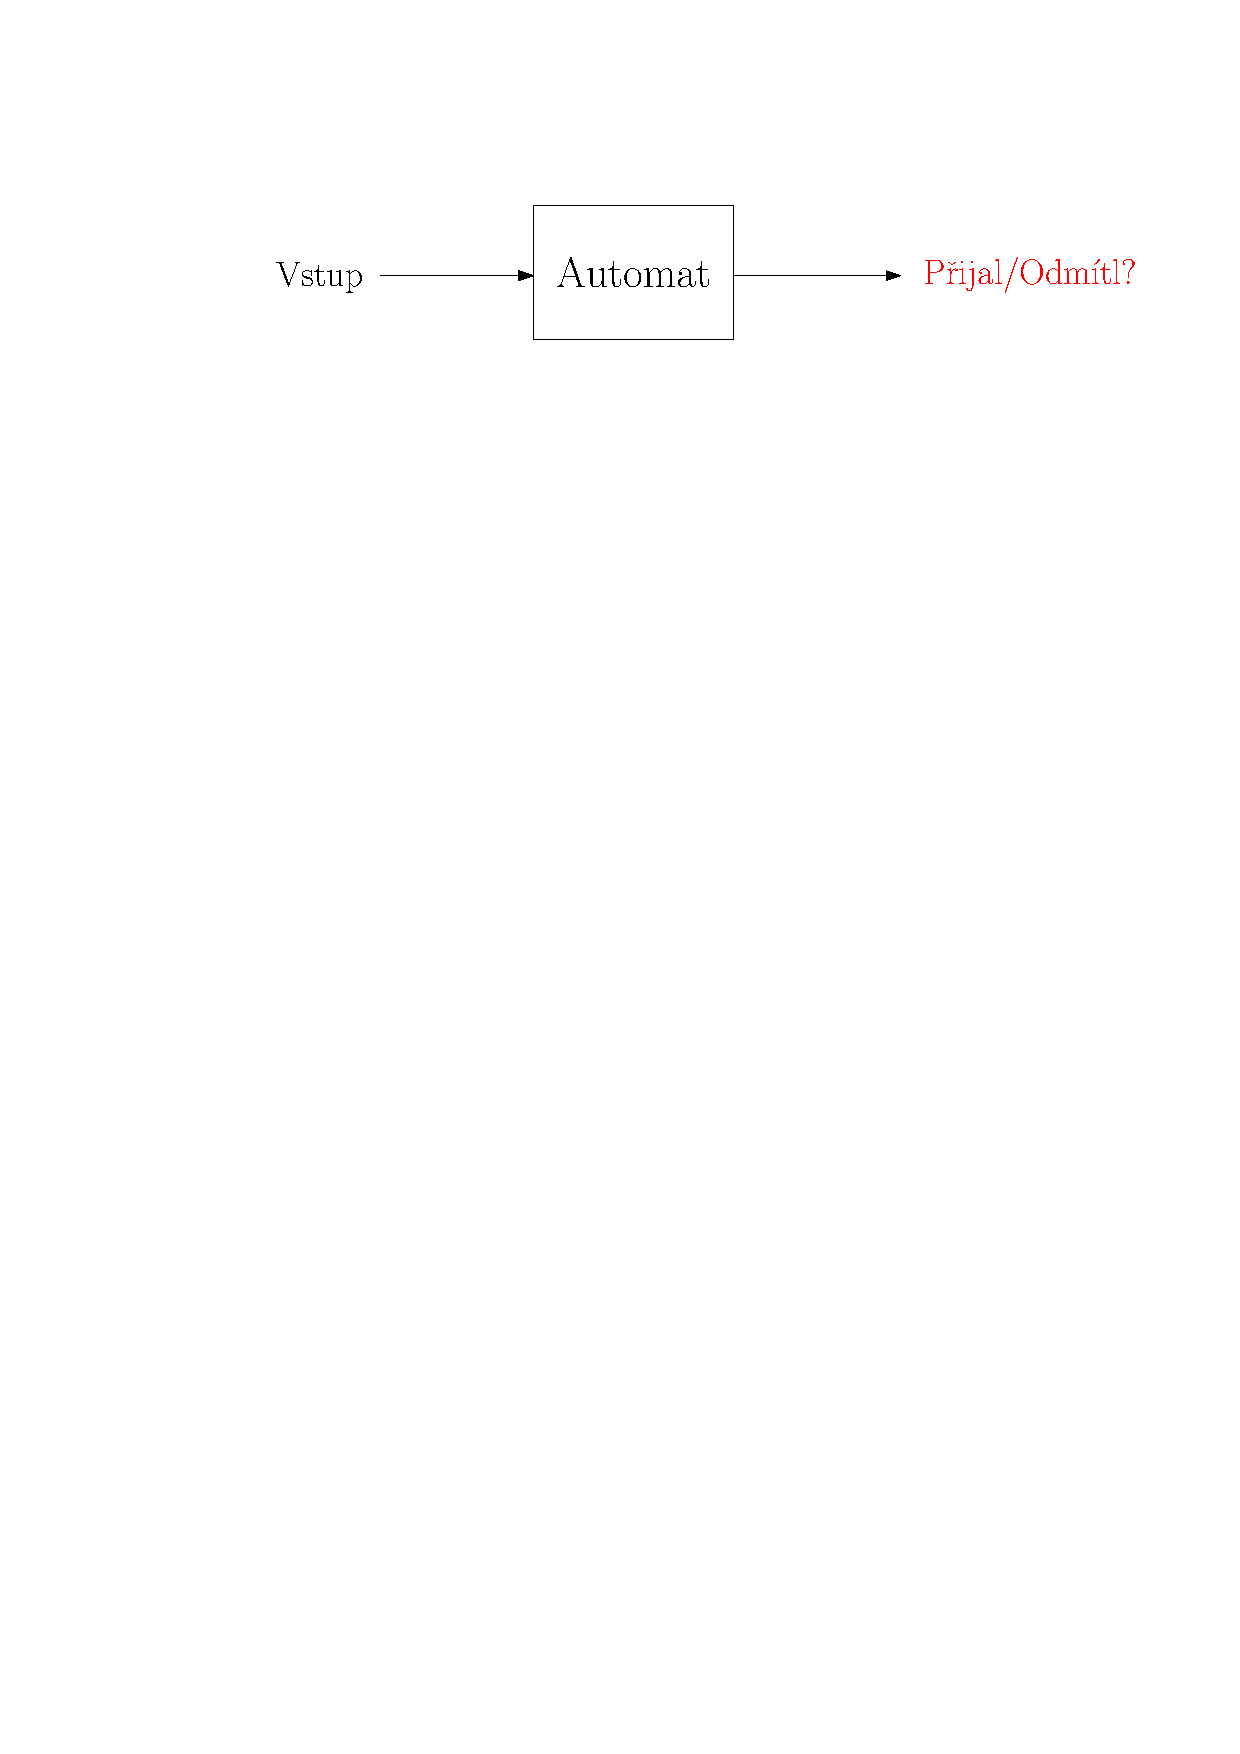
\includegraphics[scale=.7]{03-automaty/images/ch03_konecny-automat.pdf}
    \caption{Zjednodušené schéma konečného automatu.}
    \label{fig:konecny-automat}
\end{figure}
\section{Formální jazyky}\label{sec:jazyky}

Nyní, když jsme si vysvětlili základy konečných automatů a~jejich roli ve zpracovávání formálních jazyků, můžeme se hlouběji ponořit do problematiky formálních jazyků samotných. Tyto jazyky jsou totiž základem pro popis množin řetězců a~jsou klíčové pro definování toho, co automaty rozpoznávají.

Formální jazyky lze chápat jako abstraktní systémy pro popis pravidel, podle kterých jsou vytvářeny řetězce symbolů. Jsou zásadní nejen pro teorii automatů, ale také pro návrh programovacích jazyků a~kompilátorů. V~následujících částech se zaměříme na různé typy gramatik, které jsou základem pro definici formálních jazyků, a~ukážeme si, jak konečné automaty mohou tyto jazyky rozpoznávat a~zpracovávat.

Pro začátek si (jako vždy) uvedeme definice některých základních pojmů.
\begin{definition}
    Máme neprázdnou množinu znaků $\Sigma$, tzv. \textbf{abecedu}.
    \begin{itemize}
        \item \textbf{Slovo (řetězec)} je libovolná konečná posloupnost znaků ze $\Sigma$.
        \item \textbf{Prázdné slovo} je slovo neobsahující žádné znaky\footnote{Symbol $\lambda$ zde představuje speciální znak zastupující prázdné slovo. Neuvažujeme jej tedy jako součást abecedy $\Sigma$, tzn. $\lambda\notin\Sigma$.}, značíme $\lambda$.
        \item \textbf{Množina všech slov v abecedě $\Sigma$} se značí $\Sigma^*$.
        \item \textbf{Jazyk} je libovolná podmnožina slov $L\subseteq\Sigma$. Říkáme, že jazyk $L$ je \emph{nad abecedou $\Sigma$} (viz obrázek \ref{fig:jazyk}).
        \begin{figure}[h]
            \centering
            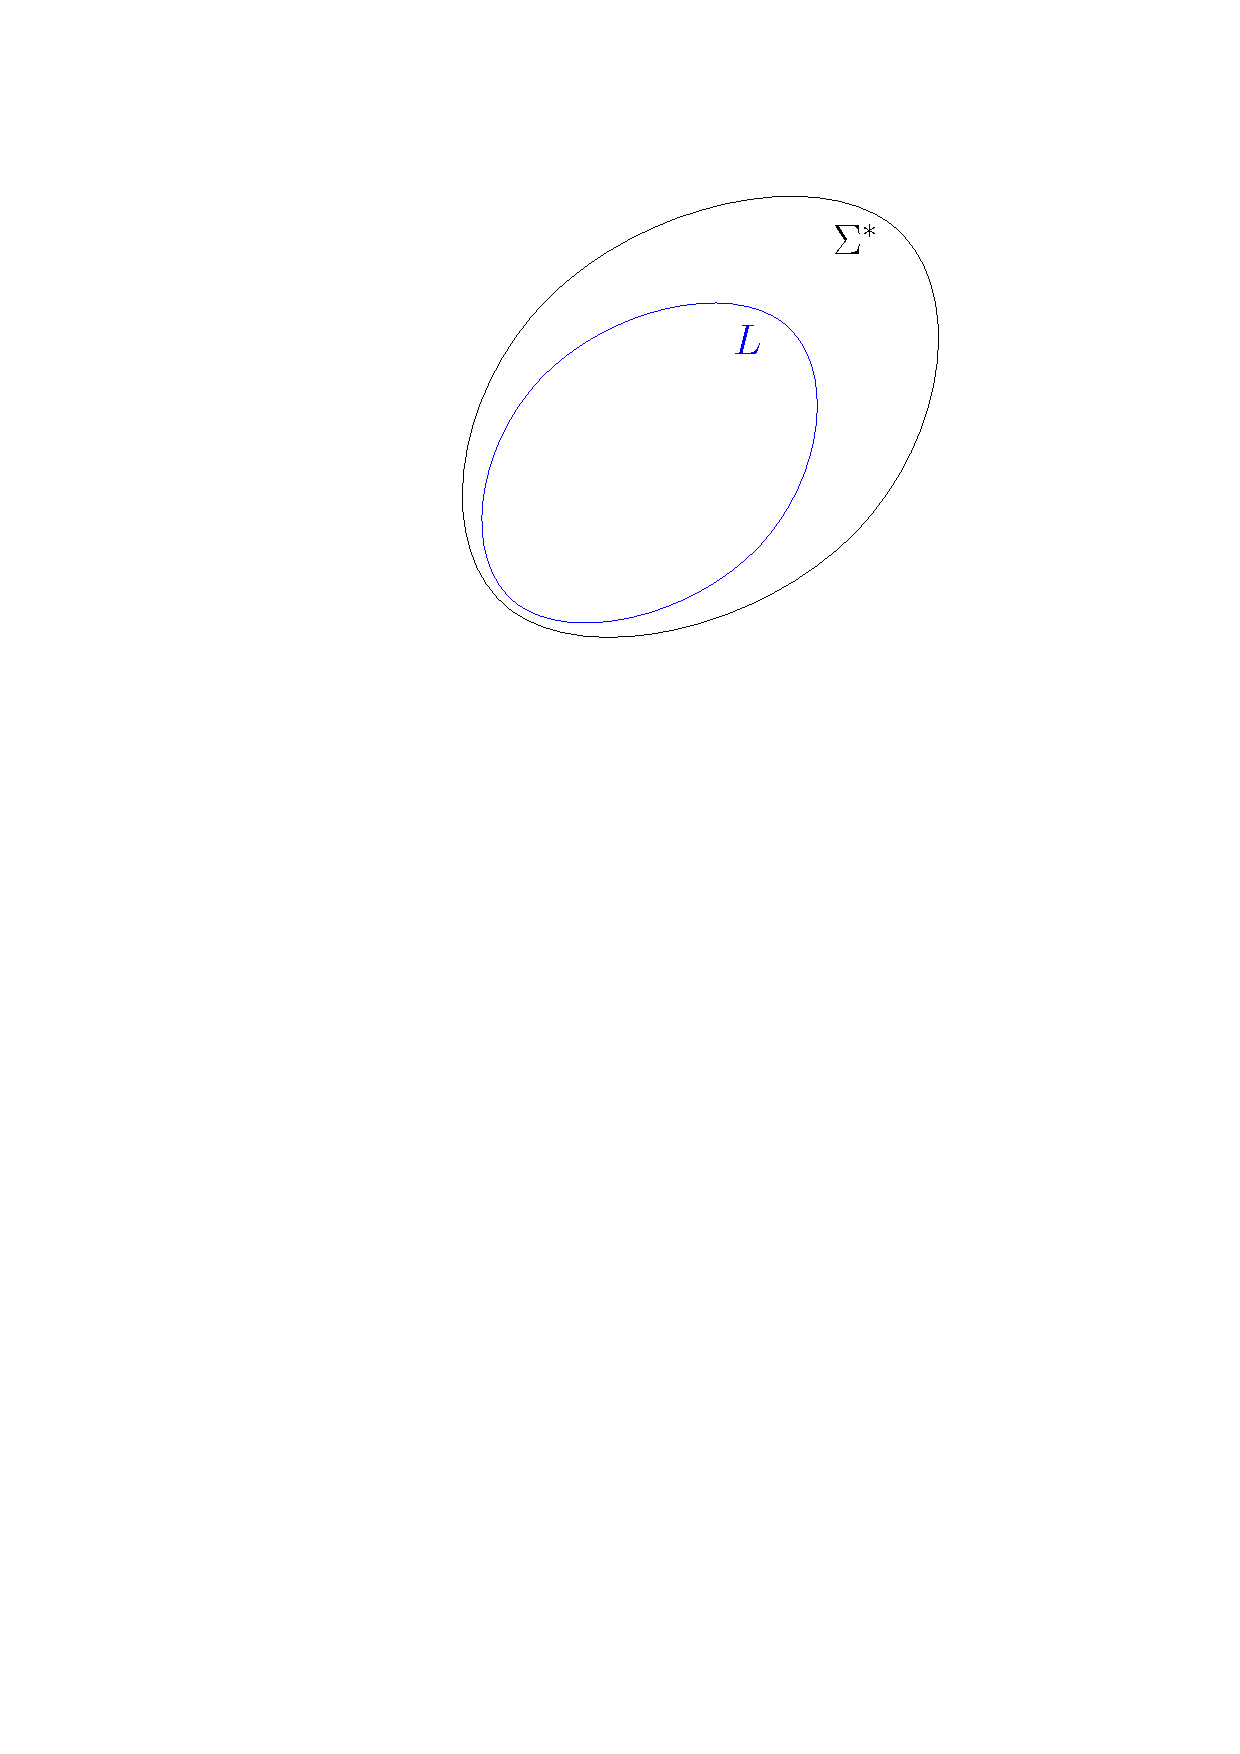
\includegraphics[scale=.7]{03-automaty/images/ch03_jazyk.pdf}
            \caption{Obecný jazyk $L$ nad abecedou $\Sigma$.}
            \label{fig:jazyk}
        \end{figure}
        \item \textbf{Délka slova} $w$ (tzn. počet znaků) se značí $|w|$.
        \item \textbf{Konkantenace} slov $u,v\in\Sigma^*$, kde $u=u_1u_2\dots u_n$ a $v=v_1v_2\dots v_m$ je slovo
        \[uv=u_1u_2\dots u_nv_1v_2\dots v_m.\]
        \item \textbf{$n$-tá mocnina} slova $u\in\Sigma^*$ je slovo
        \[u^n=\underbrace{uu\dots u}_{\text{$n$-krát}},\]
        kde $n\in\N_0$. Speciálně $u^0=\lambda$.
    \end{itemize}
\end{definition}
Podívejme se na jednoduchý příklad.
\begin{example}
    Mějme dvouznakovou abecedu $\Sigma=\set{a,b}$.
    \begin{itemize}
        \item Např. slovem v takto zadané abecedě $\Sigma$ je $w=abba$. Tzn. $|w|=4$.
        \item Množina všech slov\footnote{Je pochopiltené, že tato množina je nekonečná (délka slov není nijak omezená).} $\Sigma^*=\set{\lambda,a,b,aa,ab,ba,bb,aaa,aab,aba,\dots}$.
        \item Jednoduchý příklad jazyka nad abecedou $\Sigma$ je $L_1=\Sigma^*$, tedy všechna možná slova sestávající ze znaků $a,b$.
        \item Dalším příkladem může být např. jazyk $L_2=\set{w\in\Sigma^*\mid |w|\leqslant 2}$. Jazyk $L_2$ tedy obsahuje všechna slova délky nejvýše $2$, tj.
        \[L_2=\set{\lambda,a,b,aa,ab,ba,bb}.\]
        \item Pátá mocnina slova $w=abba$:
        \[w^5=abbaabbaabbaabbaabba.\]
        \item Konkantenace slov $u=aabb$ a $v=bbaa$
        \[uv=aabbbbaa.\]
    \end{itemize}
\end{example}

Jazyky nejsou v matematickém pojetí nic jiné než množiny objektů, tedy v tomto případě slov.
\begin{example}
    Další příklady jazyků:
    \begin{itemize}
        \item Jazyk $U=\set{w\in\Sigma^*\mid w\subseteq\set{X,Y}^*}$ obsahující všechna \emph{slova sestávající pouze z velkých písmen} nad abecedou $\Sigma=\set{x,y,X,Y}$.
        \item Jazyk $N=\set{u\in\Lambda^*\mid |u|\geqslant 1}$ obsahující všechna \emph{neprázdná slova} nad obecnou abecedou $\Lambda$ (může být jakákoliv).
        \item Jazyk $Z=\set{0^n1^n\mid n\in\N}$ nad abecedou $\Omega=\set{0,1}$.
    \end{itemize}
\end{example}
\section{Deterministické konečné automaty}\label{sec:det-automaty}

Již jsme si představili jazyky jakožto prostředek pro reprezentaci vstupů pro konečné automaty. Stále jsme si ovšem neřekli, co to ten automat vlastně je. Podobně jako v definici grafu, kdy máme uspořádanou dvojici vrcholů a hran, i zde bude myšlenka velice podobná.
\begin{definition}[Deterministický končný automat]
    \emph{Deterministický konečný automat} je uspořádaná pětice $A=(Q,\Sigma,\delta,q_0,F)$, kde
    \begin{itemize}
        \item $Q$ je konečná \emph{množina stavů},
        \item $\Sigma$ je abeceda, z níž sestávají slova na vstupu,
        \item $\delta$ je tzv. \emph{přechodová funkce} $Q\times\Sigma\rightarrow Q$ udávající přechody mezi stavy,
        \item $q_0\in Q$ je \emph{počáteční stav} automatu
        \item a $F\subseteq Q$ je \emph{množina přijímajících stavů}.
    \end{itemize}
\end{definition}
Automaty zakreslujeme pomocí stavového diagramu (formálně orientovaného grafu), přičemž
\begin{itemize}
    \item \emph{vrcholy} jsou jednotlivé stavy automatu (dvojitý kruh značí přijímající stav a do počátečního stavu vede šipka ``odnikud'')
    \item a \emph{šipky} reprezentují přechody mezi stavy.
\end{itemize}
Na začátku výpočtu dostane automat na vstupu slovo $w\in\Sigma^*$, které čte znak po znaku (zleva doprava). Začínáme v počátečním stavu $q_0$, přičemž vždy podle následujícího čteného znaku se automat přesouvá do nového stavu. Přechodová funkce $\delta:Q\times\Sigma\rightarrow Q$ nám udává pro každou dvojici $(q,a)$, kde $q$ je stav, v němž se automat nachází a $a$ je aktuálně čtený znak, do jakého stavu se má automat přesunout. Pokud na konci čtení slova $w$ skončí výpočet v jednom z přijímajících stavů, pak automat slovo přijímá. V opačném případě, kdy výpočet neskončí v přijímajícím stavu nebo přechod pro určitý znak z určitéhoi stavu není definovaný, pak výpočet končí a automat slovo nepřijímá.
\begin{example}
    Máme automat $A=(Q,\Sigma,\delta,q_0,F)$, kde
    \begin{itemize}
        \item $Q=\set{q_0,q_1,q_2}$,
        \item $q_0$ je počáteční stav,
        \item $F=\set{q_2}$,
        \item $\Sigma=\set{0,1}$,
        \item Přechodová funkce $\delta$ (viz tabulka \ref{tab:prechodova-funkce-A}):
        \begin{itemize}
            \item $\delta(q_0,0)=q_1$,
            \item $\delta(q_0,1)=q_2$,
            \item $\delta(q_0,0)=q_2$,
            \item $\delta(q_0,1)=q_2$.
        \end{itemize}
    \end{itemize}
    Schéma automatu lze vidět na obrázku \ref{fig:automat-A} níže.
    \begin{figure}[h]
        \centering
        \centering
        \begin{center}
            \begin{tikzpicture}[scale=0.2]
            \tikzstyle{every node}+=[inner sep=0pt]
            \draw [black] (18.8,-30.5) circle (3);
            \draw (18.8,-30.5) node {$q_0$};
            \draw [black] (32.6,-30.5) circle (3);
            \draw (32.6,-30.5) node {$q_1$};
            \draw [black] (46.9,-30.5) circle (3);
            \draw (46.9,-30.5) node {$q_2$};
            \draw [black] (46.9,-30.5) circle (2.4);
            \draw [black] (21.8,-30.5) -- (29.6,-30.5);
            \fill [black] (29.6,-30.5) -- (28.8,-30) -- (28.8,-31);
            \draw (25.7,-31) node [below] {$0$};
            \draw [black] (35.6,-30.5) -- (43.9,-30.5);
            \fill [black] (43.9,-30.5) -- (43.1,-30) -- (43.1,-31);
            \draw (39.75,-31) node [below] {$1$};
            \draw [black] (45.577,-27.82) arc (234:-54:2.25);
            \draw (46.9,-23.25) node [above] {$0,1$};
            \fill [black] (48.22,-27.82) -- (49.1,-27.47) -- (48.29,-26.88);
            \draw [black] (11.8,-30.5) -- (15.8,-30.5);
            \fill [black] (15.8,-30.5) -- (15,-30) -- (15,-31);
            \end{tikzpicture}
        \end{center}
        \caption{Schéma automatu $A$ a tabulka přechodové funkce $\delta$}
        \label{fig:automat-A}
    \end{figure}
    \begin{table}[h]
        \centering
        \begin{tabular}{c|cc}
        & $0$           & $1$           \\ \hline
        $q_0$      & $q_1$        & -- \\
        $q_1$      & -- & $q_2$        \\
        $q_2$      & $q_2$        & $q_2$        \\
        \end{tabular}
        \caption{Tabulka přechodové funkce $\delta$ automatu $A$}
        \label{tab:prechodova-funkce-A}
    \end{table}
\end{example}
\section{Nedeterministické konečné automaty}\label{sec:nedet-automaty}

U~deterministického automatu vede pro daný stav a~znak nejvýše jeden přechod. Někdy je však návrh mnohem jednodušší,~když automatu dovolíme několik možností a~představíme si,~že vyzkouší všechny paralelně.

\begin{definition}[Potenční množina]
    Nechť $M$ je množina. \emph{Potenční množinou} množiny $M$ nazveme množinu všech jejích podmnožin. Značíme ji
    \[
        \powset{M}=\set{N:N\subseteq M}.
    \]
    Například pro $M=\set{q_0,q_1}$ dostaneme
    \[
        \powset{M}=\set{\emptyset,\set{q_0},\set{q_1},\set{q_0,q_1}}.
    \]
\end{definition}

\begin{definition}[Nedeterministický konečný automat]
    \emph{Nedeterministický konečný automat} (zkráceně NFA) je pětice
    \[A=(Q,\Sigma,\delta,q_0,F),\]
    kde $Q$,~$\Sigma$,~$q_0$ a~$F$ mají stejný význam jako u~DFA a
    \[\delta:Q\times\Sigma\to\powset{Q}\]
    přiřazuje dvojici stavu a~znaku množinu možných následujících stavů.
\end{definition}

Přečte-li NFA ve stavu $q$ znak $a$,~výpočet se rozvětví do všech stavů z~$\delta(q,a)$. Je-li tato množina prázdná,~daná větev zanikne. Automat přijme vstupní slovo právě tehdy,~když \emph{alespoň jedna} větev po přečtení celého slova skončí v~přijímajícím stavu.

\begin{example}[Slova obsahující podslovo $101$]\label{ex:nfa-101}
    Počáteční stav $q_0$ zpracovává libovolný začátek slova. Při každé jedničce může automat zároveň \uv{uhádnout},~že právě začalo hledané podslovo,~a~spustit novou větev ve stavu $q_1$.
    \begin{figure}[h]
        \centering
        \begin{tikzpicture}
    \initialstate{q0}{(0,0)}{$q_0$}{(-1.2,0)}{180}
    \state{q1}{(2.4,0)}{$q_1$}
    \state{q2}{(4.8,0)}{$q_2$}
    \acceptingstate{q3}{(7.2,0)}{$q_3$}
    \transitionarrow[loop above]{q0}{above}{$0,1$}{q0}
    \transitionarrow{q0}{above}{$1$}{q1}
    \transitionarrow{q1}{above}{$0$}{q2}
    \transitionarrow{q2}{above}{$1$}{q3}
    \transitionarrow[loop above]{q3}{above}{$0,1$}{q3}
\end{tikzpicture}

        \caption{NFA přijímající právě slova obsahující podslovo $101$.}
        \label{fig:nfa-101}
    \end{figure}
    Pro slovo $01101$ vznikne přijímající větev,~která po posledních třech znacích projde stavy $q_1,q_2,q_3$.
\end{example}

\begin{example}[Třetí znak od konce je $1$]\label{ex:nfa-treti-od-konce}
    NFA může při každé přečtené jedničce odhadnout,~že do konce zbývají právě dva znaky. Pak už pouze odpočítá dva další přechody.
    \begin{figure}[h]
        \centering
        \begin{tikzpicture}
    \initialstate{q0}{(0,0)}{$q_0$}{(-1.2,0)}{180}
    \state{q1}{(2.5,0)}{$q_1$}
    \state{q2}{(5,0)}{$q_2$}
    \acceptingstate{q3}{(7.5,0)}{$q_3$}
    \transitionarrow[loop above]{q0}{above}{$0,1$}{q0}
    \transitionarrow{q0}{above}{$1$}{q1}
    \transitionarrow{q1}{above}{$0,1$}{q2}
    \transitionarrow{q2}{above}{$0,1$}{q3}
\end{tikzpicture}

        \caption{NFA pro jazyk slov,~jejichž třetí znak od konce je $1$.}
        \label{fig:nfa-treti-od-konce}
    \end{figure}
    Tento automat má jen čtyři stavy. Ekvivalentní DFA si musí pamatovat všechny možné konce délky tři a~potřebuje osm stavů.
\end{example}

\begin{example}[Jednoduchý zápis desetinného čísla]
    Automat na obrázku \ref{fig:automat-desetinne} přijímá neprázdný blok číslic a~případně desetinnou tečku následovanou dalším neprázdným blokem číslic. Přijme tedy \texttt{17} a~\texttt{17.25},~ale odmítne \texttt{.25},~\texttt{17.} i~\texttt{1.2.3}.
    \begin{figure}[h]
        \centering
        \begin{tikzpicture}
    \initialstate{s}{(0,0)}{$s$}{(-1.2,0)}{180}
    \acceptingstate{i}{(2.5,0)}{$q_i$}
    \state{dot}{(5,0)}{$q_t$}
    \acceptingstate{f}{(7.5,0)}{$q_f$}
    \transitionarrow{s}{above}{$0,\dots,9$}{i}
    \transitionarrow[loop above]{i}{above}{$0,\dots,9$}{i}
    \transitionarrow{i}{above}{\texttt{.}}{dot}
    \transitionarrow{dot}{above}{$0,\dots,9$}{f}
    \transitionarrow[loop above]{f}{above}{$0,\dots,9$}{f}
\end{tikzpicture}

        \caption{Konečný automat pro jednoduchý zápis nezáporného desetinného čísla.}
        \label{fig:automat-desetinne}
    \end{figure}
\end{example}

\subsection{Vztah DFA a~NFA}

Nedeterminismus sice může výrazně zjednodušit zápis automatu,~ale nerozšíří množinu jazyků,~které konečné automaty dokážou přijímat.

\begin{theorem}[Podmnožinová konstrukce]\label{thm:subset-construction}
    Ke každému NFA $A$ existuje DFA $B$ takový,~že $L(A)=L(B)$.
\end{theorem}
\begin{proof}
    Mějme NFA $A=(Q,\Sigma,\delta,q_0,F)$. Jeden stav nového DFA bude popisovat celou množinu stavů,~v~nichž se NFA může po přečtení stejného začátku slova nacházet. Položíme tedy
    \[B=(\powset{Q},\Sigma,\delta',\set{q_0},F'),\]
    kde
    \[\delta'(S,a)=\bigcup_{q\in S}\delta(q,a)\]
    a~množina $S\subseteq Q$ je přijímajícím stavem právě tehdy,~když $S\cap F\neq\emptyset$.

    Indukcí podle délky přečteného slova dostaneme,~že stav DFA $B$ je vždy přesně množinou všech stavů,~ve kterých mohou být jednotlivé větve NFA $A$. DFA proto přijme právě tehdy,~když alespoň jedna větev NFA skončí v~$F$.
\end{proof}

Každý DFA je zároveň NFA,~jen všechny množiny $\delta(q,a)$ mají nejvýše jeden prvek. Oba modely tedy přijímají stejné jazyky. Cena za odstranění nedeterminismu může být vysoká: NFA s~$n$ stavy může podmnožinovou konstrukcí vytvořit DFA až s~$2^n$ stavy.

\subsection{Přechody bez čtení znaku}

Pro důkaz Kleeneho věty se nám bude hodit ještě drobné technické rozšíření.

\begin{definition}[$\lambda$-NFA]
    \emph{$\lambda$-NFA} je NFA s~přechodovou funkcí
    \[
        \delta:Q\times(\Sigma\cup\set{\lambda})\to\powset{Q},
    \]
    který smí navíc použít přechod označený $\lambda$. Při takovém přechodu změní stav,~aniž by přečetl znak vstupu.
\end{definition}

Takový automat stále nepřijímá nic navíc. Pro množinu stavů $S$ označme $E(S)$ množinu všech stavů dosažitelných ze $S$ pouze pomocí nulového nebo více $\lambda$-přechodů. Obyčejný NFA sestrojíme tak,~že pro každý stav $q$ a~znak $a$ položíme
\[\delta'(q,a)=E\left(\bigcup_{r\in E(\set{q})}\delta(r,a)\right)\]
a~stav $q$ prohlásíme za přijímající,~pokud $E(\set{q})\cap F\neq\emptyset$. Nový automat před každým znakem i~po něm provede předem všechny možné $\lambda$-přechody,~takže přijímá tentýž jazyk.

\subsection{Regulární jazyky}

\begin{definition}[Regulární jazyk]
    Jazyk $L$ nazveme \emph{regulární},~pokud existuje DFA $A$ takový,~že $L=L(A)$.
\end{definition}

Podle věty \ref{thm:subset-construction} můžeme v~definici stejně dobře použít NFA nebo $\lambda$-NFA. Ne každý jazyk je však regulární.

\begin{theorem}\label{thm:leq-neregular}
    Jazyk
    \[L_{\mathrm{eq}}=\set{w\in\set{0,1}^*:|w|_0=|w|_1}\]
    není regulární.
\end{theorem}
\begin{proof}
    Předpokládejme pro spor,~že existuje DFA $A$ s~$m$ stavy a~$L(A)=L_{\mathrm{eq}}$. Uvažujme $m+1$ slov
    \[\lambda,0,00,\dots,0^m.\]
    Automat má jen $m$ stavů,~takže po přečtení dvou různých slov $0^i$ a~$0^j$,~kde $0\leqslant i<j\leqslant m$,~musí být ve stejném stavu.

    Nyní k~oběma slovům připojme stejný konec $1^i$. Automat z~téhož stavu čte tentýž zbytek,~a~proto buď přijme obě slova,~nebo obě odmítne. Jenže
    \[0^i1^i\in L_{\mathrm{eq}},\qquad 0^j1^i\notin L_{\mathrm{eq}}.\]
    Automat by je musel rozlišit. Dostáváme spor.
\end{proof}

\begin{figure}[h]
    \centering
    \begin{tikzpicture}[node distance=18mm]
    \node[task] (a) {$0^i$};
    \node[task,below=12mm of a] (b) {$0^j$};
    \state{q}{(3.3,-0.65)}{$q$}
    \acceptingstate{f}{(6.6,-0.65)}{$f$}
    \draw[diredge] (a) -- node[above,sloped]{čtení} (q);
    \draw[diredge] (b) -- node[below,sloped]{čtení} (q);
    \transitionarrow{q}{above}{$1^i$}{f}
    \node[below=8mm of f] {$0^i1^i\in L_{\mathrm{eq}}$, ale $0^j1^i\notin L_{\mathrm{eq}}$};
\end{tikzpicture}

    \caption{Po slovech $0^i$ a~$0^j$ je automat ve stejném stavu,~takže stejný konec $1^i$ už nedokáže rozlišit.}
\end{figure}

\section{Regulární výrazy}\label{sec:regex}
\section{Gramatiky}\label{sec:gramatiky}

\chapter{Kompilátory}\label{chap:kompilatory}
\chapter{Hardware}\label{chap:hw}
\chapter{Kryptografie}\label{chap:kryptografie}

V~\smartref[kapitole~][]{\showrefs}{chap:hw}{předchozí kapitole o~hardwaru} jsme sledovali, jak počítač ukládá a~zpracovává bity. Samotná bitová reprezentace však neříká nic o~tom, kdo smí uložená data přečíst, zda je někdo cestou změnil ani od koho skutečně pocházejí. Jakmile zprávu posíláme přes síť nebo ji ukládáme na zařízení, ke kterému mohou získat přístup další lidé, potřebujeme tyto otázky řešit výpočetními prostředky.

Právě zde nastupuje kryptografie. Nejprve si ujasníme její cíle a~doplníme základy pravděpodobnosti, bez nichž nelze moderní pojem bezpečnosti přesně formulovat. Poté začneme historickými substitučními šiframi a~přejdeme k~symetrickému a~asymetrickému šifrování. Na algoritmu RSA uvidíme, jak lze bezpečnost spojit s~obtížností matematického problému. Závěr kapitoly bude patřit pseudonáhodným generátorům, jednosměrným a~hešovacím funkcím, standardu SHA a~elektronickému podpisu.

\section{Co je to kryptografie?}\label{sec:krypto-uvod}

Název \emph{kryptologie} vznikl spojením řeckých slov označujících něco skrytého a~nauku. Kryptologie je zastřešující obor zabývající se ochranou informací i~překonáváním této ochrany. \emph{Kryptografie} zkoumá návrh a~vlastnosti metod, které mají informace chránit, zatímco \emph{kryptanalýza} hledá způsoby, jak takové metody prolomit. Tyto dvě oblasti se navzájem doplňují: šifru nelze považovat za bezpečnou jen proto, že její autor zatím žádný útok nenašel.

Základní situaci budeme popisovat pomocí tradičních postav Alice a~Boba. Alice chce Bobovi poslat zprávu
\[
    m\in\set{0,1}^{n}.
\]
Komunikační kanál však sleduje záškodník. Ten může přenášená data odposlechnout, pozměnit, zadržet nebo nahradit vlastní zprávou. Předpokládáme přitom, že záškodník zná používané algoritmy. Tajemstvím nemá být způsob šifrování, ale pouze vhodně zvolený klíč.

\begin{figure}[ht]
    \centering
    \input{06-kryptografie/images/ch06-komunikace.tex}
    \caption{Alice posílá Bobovi zprávu přes kanál sledovaný záškodníkem.}
    \label{fig:krypto-komunikace}
\end{figure}

Kryptografie neřeší pouze utajení obsahu. V~praxi se obvykle snažíme dosáhnout několika odlišných cílů:
\begin{itemize}
    \item \textbf{důvěrnost} -- obsah zprávy má být čitelný pouze oprávněným příjemcům;
    \item \textbf{integrita} -- příjemce má poznat, zda byla zpráva změněna;
    \item \textbf{autenticita} -- příjemce má umět ověřit, od koho zpráva pochází;
    \item \textbf{doložitelnost původu} -- odesílatel nemá moci snadno popřít, že zprávu vytvořil; přesný právní význam však závisí na použitém typu podpisu a~okolnostech.
\end{itemize}

Šifrování se zaměřuje především na důvěrnost, samo o~sobě však automaticky nezaručuje integritu ani autenticitu. Hešovací funkce pomáhají odhalit změnu dat, ale neříkají, kdo otisk vytvořil. Elektronický podpis propojí obsah zprávy se soukromým klíčem podepisující osoby. Jednotlivé nástroje proto budeme posuzovat podle toho, jaký bezpečnostní problém skutečně řeší.

\importantbox{Bezpečnost moderního kryptografického systému nemá stát na utajení algoritmu. Algoritmus může být veřejný a~podrobně zkoumaný; tajný zůstává klíč. Díky tomu lze systém analyzovat a~případné slabiny odhalit dříve, než budou zneužity.}

\subsection{Šifrování a~dešifrování}

Zprávu před zašifrováním nazýváme \emph{otevřený text}. Šifrovací algoritmus $\mathbf{E}$ ji spolu s~klíčem převede na \emph{šifrový text} $c$. Dešifrovací algoritmus $\mathbf{D}$ má oprávněnému příjemci umožnit získat původní zprávu:
\[
    c=\mathbf{E}(m,k),
    \qquad
    m=\mathbf{D}(c,k).
\]
Podle toho, zda se pro obě operace používá tentýž tajný klíč, nebo dvojice veřejného a~soukromého klíče, budeme později rozlišovat symetrickou a~asymetrickou kryptografii.

Požadavek na správné dešifrování nazýváme \emph{korektnost}. V~nejjednodušším symetrickém případě má pro každou dovolenou zprávu $m$ a~klíč $k$ platit
\[
    \mathbf{D}\bigl(\mathbf{E}(m,k),k\bigr)=m.
\]
Korektnost ale ještě neznamená bezpečnost. I~velmi snadno prolomitelná historická šifra může být korektní, pokud Bob se správným klíčem vždy získá původní zprávu.

\notebox{V~této kapitole pracujeme převážně s~bitovými řetězci. Text, obrázek i~jiný soubor lze před šifrováním převést na posloupnost bitů, takže model $m\in\set{0,1}^{n}$ není omezen pouze na krátké textové zprávy.}

\section{Odbočka k~pravděpodobnosti}\label{sec:krypto-pravdepodobnost}

V~historických šifrách se často ptáme, kolik klíčů musí záškodník vyzkoušet. Moderní kryptografie však používá také náhodně generované klíče a~algoritmy, které při běhu provádějí náhodné volby. Bezpečnost potom nepopisujeme pouze větou „útok je těžký“, ale pravděpodobností, s~jakou může uspět. Proto si nejprve vyložíme základní pojmy potřebné v~dalších sekcích.

\subsection{Náhodný pokus, výsledky a~jevy}

Náhodný pokus je postup, jehož konkrétní výsledek předem neznáme, přestože známe množinu všech možných výsledků. Příkladem je hod hrací kostkou, hod mincí nebo rovnoměrný výběr bitového řetězce.

\begin{definition}
    \emph{Výběrový prostor} $\Omega$ je množina všech možných výsledků náhodného pokusu. \emph{Náhodný jev} je libovolná podmnožina $A\subseteq\Omega$. Jev nastane právě tehdy, když výsledek pokusu patří do množiny $A$.
\end{definition}

Při hodu šestistěnnou kostkou máme
\[
    \Omega=\set{1,2,3,4,5,6}.
\]
Jev „padne sudé číslo“ odpovídá množině $A=\set{2,4,6}$ a~jev „padne číslo větší než čtyři“ množině $B=\set{5,6}$. Průnik $A\cap B=\set{6}$ nastane, když nastanou oba jevy současně. Sjednocení $A\cup B=\set{2,4,5,6}$ nastane, když nastane alespoň jeden z~nich.

\begin{figure}[ht]
    \centering
    \input{06-kryptografie/images/ch06-pravdepodobnost-prostor.tex}
    \caption{Výběrový prostor hodu kostkou a~dva náhodné jevy.}
    \label{fig:krypto-pravdepodobnost-prostor}
\end{figure}

\begin{definition}
    Jsou-li všechny výsledky konečného výběrového prostoru $\Omega$ stejně pravděpodobné, definujeme pravděpodobnost jevu $A\subseteq\Omega$ vztahem
    \[
        \Pr(A)=\frac{\sizeof{A}}{\sizeof{\Omega}}.
    \]
\end{definition}

Pro sudé číslo na kostce tedy dostáváme
\[
    \Pr(A)=\frac{3}{6}=\frac{1}{2}.
\]
Pravděpodobnost nemožného jevu je $\Pr(\varnothing)=0$ a~pravděpodobnost jistého jevu je $\Pr(\Omega)=1$. Často ji zapisujeme také v~procentech, například $\frac{1}{2}=50\,\%$.

Jev, že $A$ nenastane, značíme $A^\complement=\Omega\setminus A$. Platí
\[
    \Pr(A^\complement)=1-\Pr(A).
\]
Tento jednoduchý vztah bude později velmi užitečný u~narozeninového paradoxu: místo přímého počítání pravděpodobnosti, že vznikne alespoň jedna shoda, nejprve spočítáme pravděpodobnost, že nevznikne žádná.

\paragraph{Více kroků náhodného pokusu.}

Při dvou hodech mincí je potřeba rozlišovat pořadí výsledků:
\[
    \Omega=\set{00,01,10,11},
\]
kde například $01$ znamená, že v~prvním hodu padla nula a~ve druhém jednička. Jsou-li oba hody nezávislé a~obě hodnoty stejně pravděpodobné, má každý výsledek pravděpodobnost $\frac{1}{4}$.

Obecně existuje právě $2^n$ bitových řetězců délky $n$. Vybereme-li řetězec $x$ rovnoměrně náhodně z~$\set{0,1}^{n}$, potom pro každý předem zvolený řetězec $a\in\set{0,1}^{n}$ platí
\[
    \Pr_{x\in\set{0,1}^{n}}[x=a]=\frac{1}{2^n}.
\]
Dolní index zde říká, odkud a~jak náhodnou hodnotu vybíráme; výraz v~hranatých závorkách popisuje jev, jehož pravděpodobnost měříme.

\begin{example}
    Vyberme rovnoměrně náhodně $x\in\set{0,1}^{4}$. Celkem existuje $2^4=16$ možností. Jev, že $x$ začíná jedničkou, obsahuje osm řetězců, a~proto má pravděpodobnost $\frac{8}{16}=\frac{1}{2}$. Jev $x=1011$ obsahuje jediný výsledek a~má pravděpodobnost $\frac{1}{16}$.
\end{example}

\subsection{Podmíněná pravděpodobnost a~nezávislost}

Někdy už o~výsledku něco víme a~ptáme se, jak tato informace změní pravděpodobnost jiného jevu. Jestliže například víme, že na kostce padlo sudé číslo, zůstávají možné jen výsledky $\set{2,4,6}$.

\begin{definition}
    Nechť $A,B\subseteq\Omega$ a~$\Pr(B)>0$. \emph{Podmíněnou pravděpodobnost} jevu $A$ za podmínky $B$ definujeme jako
    \[
        \Pr(A\mid B)=\frac{\Pr(A\cap B)}{\Pr(B)}.
    \]
\end{definition}

Pro jevy $A=\set{2,4,6}$ a~$B=\set{4,5,6}$ při hodu kostkou je $A\cap B=\set{4,6}$. Proto
\[
    \Pr(A\mid B)
    =
    \frac{\Pr(\set{4,6})}{\Pr(\set{4,5,6})}
    =
    \frac{2/6}{3/6}
    =
    \frac{2}{3}.
\]

\begin{definition}
    Jevy $A$ a~$B$ jsou \emph{nezávislé}, jestliže informace o~nastání jednoho nemění pravděpodobnost druhého, tedy
    \[
        \Pr(A\mid B)=\Pr(A).
    \]
    Je-li $\Pr(B)>0$, je tato podmínka ekvivalentní rovnosti
    \[
        \Pr(A\cap B)=\Pr(A)\Pr(B).
    \]
\end{definition}

\begin{figure}[ht]
    \centering
    \begin{tikzpicture}[
    font=\small,
    level 1/.style={sibling distance=6cm, level distance=1.4cm},
    level 2/.style={sibling distance=2.7cm, level distance=1.4cm},
    every node/.style={align=center},
    result/.style={rounded corners=1mm, draw=blue!60!black, fill=blue!10,
                   minimum width=1.2cm, minimum height=6mm},
    edge from parent/.style={draw=black!70, -{Latex}}
]
    \node {\(\Omega\)}
        child {node {\(0\)}
            child {node[result] {\(00\)\\\(\frac14\)}
                edge from parent node[left] {\(\frac12\)}}
            child {node[result] {\(01\)\\\(\frac14\)}
                edge from parent node[right] {\(\frac12\)}}
            edge from parent node[left] {\(\frac12\)}
        }
        child {node {\(1\)}
            child {node[result] {\(10\)\\\(\frac14\)}
                edge from parent node[left] {\(\frac12\)}}
            child {node[result] {\(11\)\\\(\frac14\)}
                edge from parent node[right] {\(\frac12\)}}
            edge from parent node[right] {\(\frac12\)}
        };
\end{tikzpicture}

    \caption{Dva nezávislé hody mincí a~pravděpodobnosti výsledných řetězců.}
    \label{fig:krypto-pravdepodobnost-strom}
\end{figure}

V~kryptografii je nezávislost klíče na zprávě zásadní. Pokud by volba klíče závisela na obsahu zprávy, mohl by způsob jeho generování sám prozrazovat informace. U~jednorázové šifry budeme dokonce požadovat, aby znalost šifrového textu nezměnila pravděpodobnost žádné původní zprávy:
\[
    \Pr(M=m\mid C=c)=\Pr(M=m).
\]

\paragraph{Náhodné veličiny.}

\begin{definition}
    \emph{Náhodná veličina} přiřazuje každému výsledku náhodného pokusu nějakou hodnotu. Formálně jde o~zobrazení $\mapping{X}{\Omega}{S}$, kde $S$ je množina možných hodnot veličiny.
\end{definition}

Písmena $M$, $K$ a~$C$ budeme používat pro náhodné veličiny představující postupně zprávu, klíč a~šifrový text. Zápis $M=m$ označuje jev, že náhodná veličina $M$ nabyla konkrétní hodnoty $m$. Rozdíl mezi $M$ a~$m$ je tedy podobný rozdílu mezi proměnnou a~její právě zvolenou hodnotou.

\notebox{Pravděpodobnostní algoritmus může při běhu používat vlastní náhodné bity. Pokud píšeme pravděpodobnost jeho úspěchu, počítáme nejen s~náhodným vstupem, ale také s~těmito vnitřními volbami. Stejný algoritmus proto může na stejném vstupu v~různých bězích postupovat odlišně.}

\section{Historické metody}\label{sec:krypto-historicke}

Nejstarší šifry pracovaly přímo se znaky textu. Zprávu bylo možné šifrovat ručně bez počítače, jejich jednoduchost je však zároveň slabinou. Na historických metodách dobře uvidíme, proč velký počet klíčů sám o~sobě ještě nezaručuje bezpečnost.

\subsection{Substituční šifra s~posunem}

Mějme abecedu
\[
    \Sigma=\set{a_0,a_1,\ldots,a_{q-1}}
\]
a~tajný posun $k$, kde $0<k<q$. Každý znak nahradíme znakem posunutým o~$k$ míst:
\[
    a_i\longmapsto a_{(i+k)\bmod q}.
\]
Operace modulo $q$ způsobí, že se po dosažení konce abecedy vrátíme na její začátek. Dešifrování používá opačný posun:
\[
    a_j\longmapsto a_{(j-k)\bmod q}.
\]

\begin{figure}[ht]
    \centering
    \begin{tikzpicture}[
    font=\small,
    cell/.style={draw=black!55, rounded corners=.6mm,
                 minimum width=8mm, minimum height=8mm, inner sep=0pt},
    arrow/.style={-{Latex}, draw=black!65, line width=.7pt}
]
    \foreach \x/\letter in {0/A,1/B,2/C,3/D,4/E,5/F,6/G,7/H}{
        \node[cell, fill=black!4] (u\x) at (\x,0) {\letter};
    }
    \foreach \x/\letter in {0/D,1/E,2/F,3/G,4/H,5/A,6/B,7/C}{
        \node[cell, fill=green!15] (d\x) at (\x,-1.4) {\letter};
    }
    \foreach \x in {0,...,7}{
        \draw[arrow] (u\x) -- (d\x);
    }
    \node[anchor=east] at (-.65,0) {původní znak};
    \node[anchor=east] at (-.65,-1.4) {šifrový znak};
    \node[font=\small\bfseries] at (3.5,.8) {posun \(k=3\)};
\end{tikzpicture}

    \caption{Substituční šifra s~posunem $k=3$ na zkrácené abecedě.}
    \label{fig:krypto-caesar}
\end{figure}

Pro standardní latinskou abecedu a~$k=3$ například dostaneme
\[
    \texttt{TAJNE}\longmapsto\texttt{WDMQH}.
\]
Jestliže záškodník nezná klíč, může jednoduše vyzkoušet všech $q-1$ nenulových posunů. Pro $q=26$ jde pouze o~25 možností. U~dostatečně dlouhé zprávy navíc snadno pozná, který výsledek připomíná smysluplný text.

\subsection{Obecná substituční šifra}

Místo jednoho posunu můžeme zvolit libovolnou permutaci abecedy
\[
    \mapping{\pi}{\Sigma}{\Sigma}.
\]
Permutace je bijekce, takže každý znak má právě jeden zašifrovaný obraz a~každý znak šifrové abecedy má právě jeden vzor. Šifrování nahradí každý znak $a$ znakem $\pi(a)$, zatímco dešifrování používá inverzní permutaci $\pi^{-1}$.

Pro abecedu o~$q$ znacích existuje $q!$ různých permutací. U~26 písmen je to přibližně $4\cdot 10^{26}$ klíčů, takže prosté vyzkoušení všech možností už není praktické. Obecná substituce však stále zachovává strukturu původního textu: stejné znaky se vždy mění na stejné znaky, opakovaná slova vytvářejí stejné vzory a~četnosti písmen se pouze přejmenují.

\begin{figure}[ht]
    \centering
    \input{06-kryptografie/images/ch06-substituce.tex}
    \caption{Obecná substituce a~zachování četností znaků.}
    \label{fig:krypto-substituce}
\end{figure}

Uvažujme například klíč, jehož prvních několik přiřazení je
\[
    A\mapsto Q,\quad B\mapsto W,\quad C\mapsto E,\quad
    D\mapsto R,\quad E\mapsto T,\quad\ldots
\]
Pro permutaci použitou na obrázku~\ref{fig:krypto-substituce} dostáváme
\[
    \texttt{TAJEMSTVI}\longmapsto\texttt{ZQPTDLZCO}.
\]

\warningbox{Velký počet klíčů neznamená automaticky bezpečnou šifru. Obecná substituce má obrovský prostor klíčů, ale frekvenční analýza využívá vlastnosti jazyka a~nemusí jednotlivé klíče zkoušet jeden po druhém.}

\paragraph{Frekvenční analýza.}

V~delším českém textu se některá písmena objevují výrazně častěji než jiná. Jestliže se v~šifrovém textu mimořádně často vyskytuje znak \texttt{Q}, může odpovídat některému běžnému písmenu otevřeného textu. Záškodník dále sleduje dvojice a~trojice znaků, délky slov nebo opakované vzory. Každý takový poznatek zmenšuje množinu možných permutací.

Historické metody nám proto ukazují dvě důležité zásady. Bezpečnost nelze odvozovat jen z~toho, že klíčů je mnoho, a~šifra by neměla zbytečně zachovávat statistickou strukturu otevřeného textu. Moderní šifry se snaží, aby bez znalosti klíče vypadal šifrový text jako náhodná data.

\section{Symetrická kryptografie}\label{sec:krypto-symetricka}

V~symetrické kryptografii používají Alice i~Bob tentýž tajný klíč
\[
    k\in\set{0,1}^{n}.
\]
Alice vytvoří šifrový text $c=\mathbf{E}(m,k)$ a~Bob obnoví zprávu výpočtem $m=\mathbf{D}(c,k)$. Klíč proto musí znát obě strany, ale nikdo další.

\begin{figure}[ht]
    \centering
    \begin{tikzpicture}[
    font=\small,
    >=Latex,
    box/.style={rounded corners=1.2mm, draw=black!55, fill=black!4,
                minimum width=2.2cm, minimum height=9mm, align=center},
    key/.style={rounded corners=1.2mm, draw=blue!65!black, fill=blue!12,
                minimum width=2cm, minimum height=8mm, align=center},
    flow/.style={-{Latex}, line width=.9pt, draw=black!70},
    keyflow/.style={-{Latex}, dashed, line width=.8pt, draw=blue!65!black}
]
    \node[inner sep=0pt] (alice) at (-6,0)
        {
\includegraphics[height=1.35cm]{06-kryptografie/images/woman-icon.pdf}};
    \node[below=1mm of alice] {Alice};
    \node[inner sep=0pt] (bob) at (6,0)
        {
\includegraphics[height=1.35cm]{06-kryptografie/images/man-icon.pdf}};
    \node[below=1mm of bob] {Bob};

    \node[box] (enc) at (-2.7,0) {\(\mathbf E(m,k)\)};
    \node[box] (dec) at (2.7,0) {\(\mathbf D(c,k)\)};
    \node[key] (key) at (0,1.65) {sdílený tajný klíč \(k\)};

    \draw[flow] (alice.east) -- (enc.west) node[midway, above] {\(m\)};
    \draw[flow] (enc.east) -- (dec.west) node[midway, above] {\(c\)};
    \draw[flow] (dec.east) -- (bob.west) node[midway, above] {\(m\)};
    \draw[keyflow] (key.south west) -- (enc.north);
    \draw[keyflow] (key.south east) -- (dec.north);

    \node[inner sep=0pt] (attacker) at (0,-2)
        {
\includegraphics[height=1.1cm]{06-kryptografie/images/hacker-icon.pdf}};
    \draw[->, red!75!black, line width=.8pt] (attacker.north)
        -- (0,-.15);
    \node[below=1mm of attacker] {zachytí pouze \(c\)};
\end{tikzpicture}

    \caption{Základní schéma symetrického šifrování.}
    \label{fig:krypto-symetricka}
\end{figure}

Symetrické algoritmy jsou obvykle velmi rychlé a~hodí se pro šifrování velkého množství dat. Hlavní organizační problém spočívá v~bezpečném předání klíče. Pokud Alice dokáže Bobovi tajně poslat dlouhý klíč, nabízí se otázka, proč stejným bezpečným kanálem neposlat přímo zprávu. Tento problém bude zvlášť dobře vidět u~jednorázové šifry.

\subsection{Operace XOR}

Jednorázová šifra používá operaci XOR, značenou symbolem $\oplus$. Pro jednotlivé bity platí
\[
\begin{array}{c|c|c}
    a & b & a\oplus b\\
    \hline
    0 & 0 & 0\\
    0 & 1 & 1\\
    1 & 0 & 1\\
    1 & 1 & 0
\end{array}
\]
Operaci na stejně dlouhých bitových řetězcích provádíme po jednotlivých pozicích. Důležitá je rovnost
\[
    (a\oplus b)\oplus b=a,
\]
protože $b\oplus b=0$ a~$a\oplus 0=a$.

\subsection{Jednorázová šifra}

Alice a~Bob sdílejí rovnoměrně náhodný tajný klíč
\[
    k\in\set{0,1}^{n},
\]
který je stejně dlouhý jako zpráva $m\in\set{0,1}^{n}$. Alice šifruje
\[
    c=m\oplus k.
\]
Bob použije stejný klíč a~spočítá
\[
    c\oplus k=(m\oplus k)\oplus k=m.
\]
Anglicky se tato metoda nazývá \emph{one-time pad}; český název zdůrazňuje, že každý klíč smí být použit právě jednou.

\begin{figure}[ht]
    \centering
    \input{06-kryptografie/images/ch06-otp.tex}
    \caption{Šifrování a~dešifrování jednorázovou šifrou.}
    \label{fig:krypto-otp}
\end{figure}

\begin{proposition}
    Nechť je $K$ rovnoměrně náhodný na $\set{0,1}^{n}$ a~nezávislý na náhodné veličině $M$. Položme $C=M\oplus K$. Potom pro každé $m,c\in\set{0,1}^{n}$ s~$\Pr(M=m)>0$ platí
    \[
        \Pr(M=m\mid C=c)=\Pr(M=m).
    \]
\end{proposition}

\begin{proof}
    Pro pevně zvolené hodnoty $m$ a~$c$ existuje právě jeden klíč, který zprávu $m$ převede na $c$, totiž
    \[
        k=m\oplus c.
    \]
    Protože je $K$ rovnoměrně náhodný a~nezávislý na $M$, dostáváme
    \[
        \Pr(M=m\ \text{a}\ C=c)
        =
        \Pr(M=m)\Pr(K=m\oplus c)
        =
        \frac{\Pr(M=m)}{2^n}.
    \]
    Dále sečteme přes všechny možné zprávy $m'$:
    \[
        \Pr(C=c)
        =
        \sum_{m'\in\set{0,1}^{n}}
        \frac{\Pr(M=m')}{2^n}
        =
        \frac{1}{2^n}.
    \]
    Z~definice podmíněné pravděpodobnosti tedy plyne
    \[
        \Pr(M=m\mid C=c)
        =
        \frac{\Pr(M=m\ \text{a}\ C=c)}{\Pr(C=c)}
        =
        \Pr(M=m).
    \]
\end{proof}

Zachycený šifrový text tedy nezmění pravděpodobnost žádné původní zprávy. Jednorázová šifra poskytuje \emph{perfektní utajení}: její bezpečnost není založena na omezeném výpočetním výkonu záškodníka. Platí dokonce proti protivníkovi s~libovolně výkonným počítačem.

\importantbox{Perfektní utajení platí pouze tehdy, když je klíč skutečně náhodný, stejně dlouhý jako zpráva, nezávislý na zprávě, bezpečně sdílený a~použitý právě jednou.}

\subsection{Proč se klíč nesmí opakovat?}

Zašifruje-li Alice dvě zprávy týmž klíčem $k$, dostaneme
\[
    c_1=m_1\oplus k,
    \qquad
    c_2=m_2\oplus k.
\]
Záškodník může oba zachycené texty spojit:
\[
    c_1\oplus c_2
    =
    (m_1\oplus k)\oplus(m_2\oplus k)
    =
    m_1\oplus m_2.
\]
Klíč se vyruší. Záškodník sice nemusí okamžitě znát obě zprávy, získá však informaci o~jejich vzájemném vztahu. Pokud jednu z~nich zná nebo správně odhadne, dopočítá druhou.

\begin{figure}[ht]
    \centering
    \input{06-kryptografie/images/ch06-opakovany-klic.tex}
    \caption{Opakované použití klíče odstraní z~výrazu neznámé $k$.}
    \label{fig:krypto-opakovany-klic}
\end{figure}

Nevýhodou jednorázové šifry je nutnost bezpečně sdílet náhodný klíč délky celé zprávy. V~\smartref[sekci~][]{\showrefs}{sec:krypto-prg-owf}{dalším výkladu} uvidíme, jak lze perfektní bezpečnost nahradit bezpečností výpočetní a~dlouhý náhodný klíč krátkým seedem.

\section{Asymetrická kryptografie}\label{sec:krypto-asymetricka}

Symetrické šifrování předpokládá, že Alice a~Bob už sdílejí tajný klíč. Asymetrická kryptografie tento požadavek mění. Každý uživatel si vytvoří dvojici vzájemně souvisejících klíčů:
\[
    \text{veřejný klíč }k_V
    \qquad\text{a}\qquad
    \text{soukromý klíč }k_S.
\]
Veřejný klíč smí znát kdokoliv, soukromý klíč si jeho vlastník musí ponechat pouze pro sebe.

Chce-li Alice poslat zprávu Bobovi, získá Bobův veřejný klíč $k_V$ a~spočítá
\[
    c=\mathbf{E}(m,k_V).
\]
Bob použije svůj soukromý klíč:
\[
    m=\mathbf{D}(c,k_S).
\]
Korektnost požaduje
\[
    \mathbf{D}\bigl(\mathbf{E}(m,k_V),k_S\bigr)=m.
\]

\begin{figure}[ht]
    \centering
    \begin{tikzpicture}[
    font=\small,
    >=Latex,
    box/.style={rounded corners=1.2mm, draw=black!55, fill=black!4,
                minimum width=2.5cm, minimum height=9mm, align=center},
    public/.style={rounded corners=1.2mm, draw=blue!65!black, fill=blue!12,
                   minimum width=2.5cm, minimum height=8mm, align=center},
    private/.style={rounded corners=1.2mm, draw=red!70!black, fill=red!9,
                    minimum width=2.5cm, minimum height=8mm, align=center},
    flow/.style={-{Latex}, draw=black!70, line width=.9pt},
    keyflow/.style={-{Latex}, dashed, line width=.8pt}
]
    \node[inner sep=0pt] (alice) at (-6,0)
        {
\includegraphics[height=1.35cm]{06-kryptografie/images/woman-icon.pdf}};
    \node[below=1mm of alice] {Alice};
    \node[inner sep=0pt] (bob) at (6,0)
        {
\includegraphics[height=1.35cm]{06-kryptografie/images/man-icon.pdf}};
    \node[below=1mm of bob] {Bob};

    \node[box] (enc) at (-2.6,0) {\(\mathbf E(m,k_V)\)};
    \node[box] (dec) at (2.6,0) {\(\mathbf D(c,k_S)\)};
    \node[public] (pk) at (-2.6,1.65) {Bobův veřejný klíč \(k_V\)};
    \node[private] (sk) at (2.6,1.65) {Bobův soukromý klíč \(k_S\)};

    \draw[flow] (alice.east) -- (enc.west) node[midway, above] {\(m\)};
    \draw[flow] (enc.east) -- (dec.west) node[midway, above] {\(c\)};
    \draw[flow] (dec.east) -- (bob.west) node[midway, above] {\(m\)};
    \draw[keyflow, draw=blue!65!black] (pk) -- (enc);
    \draw[keyflow, draw=red!70!black] (sk) -- (dec);
\end{tikzpicture}

    \caption{Šifrování Bobovým veřejným klíčem a~dešifrování jeho soukromým klíčem.}
    \label{fig:krypto-asymetricka}
\end{figure}

Znalost veřejného klíče umožňuje zprávy pro Boba šifrovat, nesmí však umožnit je efektivně dešifrovat ani odvodit $k_S$. Asymetrie tedy není v~tom, že by jedna operace byla matematicky nemožná, ale v~rozdílu výpočetní obtížnosti: s~tajnou informací je dešifrování snadné, bez ní má být prakticky neproveditelné.

\warningbox{Veřejný klíč musí být spolehlivě spojen s~identitou svého vlastníka. Pokud záškodník podstrčí Alici svůj klíč a~vydává jej za Bobův, může zprávu přečíst a~teprve potom ji znovu zašifrovat skutečným Bobovým klíčem. K~ověřování vazby mezi identitou a~veřejným klíčem se používají certifikáty.}

Asymetrické operace bývají výrazně pomalejší než symetrické. Reálné systémy proto často používají oba přístupy společně: asymetrická kryptografie bezpečně ustaví krátký dočasný klíč a~samotná data se potom šifrují rychlou symetrickou šifrou. V~této kapitole se soustředíme na princip; podrobnosti konkrétních síťových protokolů ponecháme stranou.

\subsection{Výpočetní bezpečnost}

U~jednorázové šifry jsme dokázali, že šifrový text neposkytuje žádnou informaci ani neomezeně silnému záškodníkovi. U~asymetrické kryptografie tak silný požadavek splnit nemůžeme: veřejný klíč i~algoritmus šifrování jsou dostupné, takže záškodník může kandidátní zprávy sám šifrovat a~porovnávat.

Bezpečnost proto formulujeme vůči algoritmům s~omezenou dobou výpočtu. Pravděpodobnost úspěchu každého pravděpodobnostního polynomiálního útoku má být zanedbatelná. Tato myšlenka se naplno projeví v~\smartref[sekci~][]{\showrefs}{sec:krypto-prg-owf}{sekci o~pseudonáhodných generátorech a~jednosměrných funkcích}.

\notebox{Jednoduchý zápis $c=\mathbf{E}(m,k_V)$ nezobrazuje všechny praktické podrobnosti. Bezpečné asymetrické šifrování obvykle používá také náhodnost a~předepsané kódování zprávy, aby stejné zprávy nevytvářely pokaždé stejný šifrový text.}

\section{Algoritmus RSA}\label{sec:krypto-rsa}

RSA je nejznámější příklad asymetrického kryptografického systému. Jeho název vznikl z~příjmení autorů Rona \textbf{R}ivesta, Adiho \textbf{S}hamira a~Leonarda \textbf{A}dlemana. Základní operací je umocňování modulo součin dvou velkých prvočísel.

\subsection{Vytvoření klíčů}

Bob postupuje následovně:
\begin{enumerate}
    \item zvolí dvě různá velká prvočísla $p$ a~$q$ a~spočítá
    \[
        n=pq;
    \]
    \item spočítá
    \[
        \varphi(n)=(p-1)(q-1);
    \]
    \item zvolí číslo $s$ nesoudělné s~$\varphi(n)$;
    \item nalezne číslo $v$ takové, že
    \[
        vs\bmod\varphi(n)=1;
    \]
    \item zveřejní klíč $k_V=(v,n)$ a~uchová v~tajnosti klíč $k_S=(s,n)$.
\end{enumerate}

Číslo $v$ je multiplikativní inverze čísla $s$ modulo $\varphi(n)$. Existuje právě proto, že $\operatorname{gcd}(s,\varphi(n))=1$, a~lze je efektivně nalézt rozšířeným Eukleidovým algoritmem.

\warningbox{Číslo $s$ je soukromý exponent, nikoli třetí prvočíslo. Musí být nesoudělné s~$(p-1)(q-1)$, ale samo prvočíslem být nemusí.}

\subsection{Šifrování a~dešifrování}

Zprávu reprezentujeme číslem $x$ splňujícím $0\leqslant x<n$. Alice zašifruje
\[
    y=\mathbf{E}(x,k_V)=x^v\bmod n.
\]
Bob dešifruje
\[
    \mathbf{D}(y,k_S)=y^s\bmod n.
\]
Mocniny mohou být obrovské, v~programu je však nepočítáme nejprve jako běžná celá čísla. Opakovaným umocňováním a~průběžným výpočtem zbytku lze modulární mocninu určit v~čase polynomiálním vzhledem k~počtu bitů vstupu.

\begin{figure}[ht]
    \centering
    \input{06-kryptografie/images/ch06-rsa-schema.tex}
    \caption{Schéma šifrování a~dešifrování v~RSA.}
    \label{fig:krypto-rsa-schema}
\end{figure}

\subsection{Malá Fermatova věta a~čínská věta o~zbytcích}

Korektnost RSA odvodíme ze dvou vět elementární teorie čísel.

\begin{theorem}[Malá Fermatova věta]\label{thm:krypto-fermat}
    Nechť $p$ je prvočíslo a~$a\in\Z$ není dělitelné číslem $p$. Potom
    \[
        a^{p-1}\bmod p=1.
    \]
    Ekvivalentně pro každé $a\in\Z$ platí $a^p\bmod p=a\bmod p$.
\end{theorem}

\begin{theorem}[Čínská věta o~zbytcích]\label{thm:krypto-cinska}
    Nechť $m_1,\ldots,m_k\in\N$ jsou po dvou nesoudělná. Pro libovolná $a_1,\ldots,a_k\in\Z$ existuje řešení soustavy
    \[
        x\equiv a_i\pmod{m_i},
        \qquad i=1,\ldots,k,
    \]
    a~všechna její řešení jsou navzájem shodná modulo $M=m_1\cdots m_k$.
\end{theorem}

\begin{corollary}\label{cor:krypto-cinska-dve}
    Jsou-li $p$ a~$q$ různá prvočísla a~platí
    \[
        a\equiv b\pmod p
        \qquad\text{a}\qquad
        a\equiv b\pmod q,
    \]
    potom $a\equiv b\pmod{pq}$.
\end{corollary}

\subsection{Korektnost RSA}

\begin{theorem}\label{thm:krypto-rsa-korektnost}
    Pro klíče vytvořené uvedeným postupem a~každé celé číslo $x$ splňující $0\leqslant x<n$ platí
    \[
        \mathbf{D}\bigl(\mathbf{E}(x,k_V),k_S\bigr)=x.
    \]
\end{theorem}

\begin{proof}
    Z~rovnosti $vs\bmod(p-1)(q-1)=1$ plyne, že pro nějaké $t\in\N_0$ platí
    \[
        vs=1+t(p-1)(q-1).
    \]
    Nejprve ukážeme $x^{vs}\equiv x\pmod p$. Pokud $p$ dělí $x$, jsou obě strany kongruence nulové modulo $p$. Pokud $p$ číslo $x$ nedělí, použijeme \smartref[větu~][]{\showrefs}{thm:krypto-fermat}{malou Fermatovu větu}:
    \begin{align*}
        x^{vs}
        &=
        x^{1+t(p-1)(q-1)}\\
        &=
        x\left(x^{p-1}\right)^{t(q-1)}
        \equiv
        x\cdot 1^{t(q-1)}
        \equiv x
        \pmod p.
    \end{align*}
    Stejným rozlišením případů dostaneme
    \[
        x^{vs}\equiv x\pmod q.
    \]
    Podle \smartref[důsledku~][]{\showrefs}{cor:krypto-cinska-dve}{důsledku čínské věty o~zbytcích} tedy
    \[
        x^{vs}\equiv x\pmod{pq}.
    \]
    Protože $n=pq$ a~$0\leqslant x<n$, uzavíráme
    \[
        \mathbf{D}\bigl(\mathbf{E}(x,k_V),k_S\bigr)
        =
        \left(x^v\bmod n\right)^s\bmod n
        =
        x^{vs}\bmod n
        =
        x.
    \]
\end{proof}

\begin{figure}[ht]
    \centering
    \begin{tikzpicture}[
    font=\small,
    >=Latex,
    box/.style={rounded corners=1.2mm, draw=black!55, fill=black!4,
                minimum width=3.3cm, minimum height=9mm, align=center},
    residue/.style={rounded corners=1.2mm, draw=blue!65!black, fill=blue!11,
                    minimum width=4.1cm, minimum height=10mm, align=center},
    result/.style={rounded corners=1.2mm, draw=green!55!black, fill=green!12,
                   minimum width=5cm, minimum height=10mm, align=center},
    flow/.style={-{Latex}, draw=black!70, line width=.9pt}
]
    \node[box] (power) at (0,2.2) {\(x^{vs}\), kde \(vs=1+t(p-1)(q-1)\)};
    \node[residue] (p) at (-3.3,.25)
        {\(x^{vs}\equiv x\pmod p\)\\malá Fermatova věta};
    \node[residue] (q) at (3.3,.25)
        {\(x^{vs}\equiv x\pmod q\)\\malá Fermatova věta};
    \node[result] (pq) at (0,-2)
        {\(x^{vs}\equiv x\pmod{pq}\)\\čínská věta o~zbytcích};

    \draw[flow] (power.south west) -- (p.north);
    \draw[flow] (power.south east) -- (q.north);
    \draw[flow] (p.south) -- (pq.north west);
    \draw[flow] (q.south) -- (pq.north east);
\end{tikzpicture}

    \caption{Myšlenka důkazu korektnosti RSA přes moduly $p$, $q$ a~$pq$.}
    \label{fig:krypto-rsa-korektnost}
\end{figure}

\paragraph{Příklad s~malými čísly.}

\begin{example}
    Zvolme $p=5$, $q=11$ a~$s=27$. Potom
    \[
        n=55,
        \qquad
        \varphi(n)=(5-1)(11-1)=40.
    \]
    Protože $\operatorname{gcd}(27,40)=1$, můžeme nalézt $v$ splňující
    \[
        27v\bmod 40=1.
    \]
    Vyhovuje $v=3$, neboť $27\cdot 3=81\equiv 1\pmod{40}$. Veřejný klíč je $k_V=(3,55)$ a~soukromý klíč $k_S=(27,55)$.

    Alice zašifruje $x=7$:
    \[
        y=7^3\bmod 55=343\bmod 55=13.
    \]
    Bob poté získá
    \[
        13^{27}\bmod 55=7.
    \]
\end{example}

Malá čísla slouží pouze k~ručnímu ověření postupu. V~reálné kryptografii by tak malý modul záškodník rozložil okamžitě.

\subsection{Bezpečnost a~faktorizace}

Veřejný klíč obsahuje $n=pq$, ale nikoli samotná prvočísla $p$ a~$q$. Pokud záškodník rozklad zjistí, spočítá $\varphi(n)=(p-1)(q-1)$ a~z~veřejného exponentu $v$ odvodí soukromý exponent $s$. Efektivní faktorizace by tedy RSA prolomila.

Rozhodovací verzi problému můžeme zapsat takto:
\[
    \FACTOR:
    \quad
    \text{pro daná }n,b\in\N\text{ rozhodni, zda existuje }d
    \text{ takové, že }1<d<b\text{ a }d\mid n.
\]
Jak jsme viděli v~\smartref[sekci~][]{\showrefs}{sec:p_np}{dřívějším výkladu tříd P a~NP}, kladnou odpověď stačí doložit dělitelem $d$. Ověření nerovností i~rovnosti $n\bmod d=0$ proběhne v~polynomiálním čase, a~proto $\FACTOR\in\classNP$.

Naivní zkoušení dělitelů je vzhledem k~bitové délce $\sizeof{\binarycode{n}}$ exponenciální. Jsou známy podstatně rychlejší klasické algoritmy, žádný obecný polynomiální klasický algoritmus pro faktorizaci však znám není.

\importantbox{Znalost efektivní faktorizace stačí k~prolomení popsaného RSA. Není však dokázáno, že každý způsob, jak invertovat RSA, musí zároveň faktorizovat $n$. Bezpečnost RSA proto nelze jednoduše ztotožnit s~větou „faktorizace je těžká“.}

\warningbox{Uvedené „učebnicové RSA“ je deterministické a~bez doplňujícího kódování není bezpečným praktickým šifrovacím schématem. Skutečné systémy používají standardizované náhodné vycpávání a~oddělené postupy, například OAEP pro šifrování a~PSS pro podpis.}

\section{Pseudonáhodné generátory a~jednosměrné funkce}\label{sec:krypto-prg-owf}

Jednorázová šifra ukázala, že dlouhý rovnoměrně náhodný klíč dokáže skrýt zprávu dokonale. Zároveň jsme narazili na její zásadní omezení: pro zprávu délky $n$ potřebujeme předem sdílet $n$ náhodných bitů. Moderní kryptografie se proto vzdává absolutního požadavku, aby šifrový text neobsahoval vůbec žádnou informaci, a~nahrazuje jej požadavkem výpočetním. Připouštíme, že informace může být v~principu zjistitelná, ale žádný dostatečně rychlý algoritmus ji nemá umět prakticky využít.

Tento posun je zásadní. Výpočetní složitost zde není překážkou, kterou se snažíme odstranit, nýbrž prostředkem ochrany. Oprávněný uživatel zná krátký klíč nebo zvláštní tajnou informaci a~výpočet provede rychle. Záškodník stejnou informaci nemá a~stojí před úlohou, pro kterou neznáme efektivní postup.

Technické definice v~této sekci vyjadřují tři myšlenky:
\begin{enumerate}
    \item oprávněný výpočet musí probíhat v~polynomiálním čase;
    \item záškodník smí používat libovolný pravděpodobnostní polynomiální algoritmus;
    \item pravděpodobnost jeho úspěchu musí s~rostoucí délkou vstupu klesat rychleji než převrácená hodnota libovolného polynomu.
\end{enumerate}
Poslední bod zachytíme pojmem zanedbatelné funkce.

\subsection{Zanedbatelná funkce}

\begin{definition}\label{def:krypto-zanedbatelna}
    Funkce $\mapping{\varepsilon}{\N}{\R}$ je \emph{zanedbatelná}, jestliže pro každé $k\in\N$ existuje $n_k\in\N$ takové, že pro každé $n>n_k$ platí
    \[
        \sizeof{\varepsilon(n)}<\frac{1}{n^k}.
    \]
\end{definition}

Zanedbatelná funkce tedy nakonec klesne pod $\frac{1}{n}$, pod $\frac{1}{n^2}$, pod $\frac{1}{n^{100}}$ i~pod převrácenou hodnotu jakéhokoliv jiného pevně zvoleného polynomu. Typickým příkladem je $2^{-n}$. Naopak funkce $\frac{1}{n^{10}}$ zanedbatelná není, protože pro $k=11$ nikdy dlouhodobě neklesne pod $\frac{1}{n^{11}}$.

Číslo $n$ zde hraje roli \emph{bezpečnostního parametru}. Jeho zvětšením prodlužujeme klíče a~zvyšujeme množství práce potřebné k~útoku. Tvrzení o~zanedbatelné pravděpodobnosti neznamená, že útok nemůže nikdy uspět; říká, že jeho šanci lze volbou dostatečně velkého parametru stlačit pod každou prakticky významnou inverzní polynomiální mez.

\subsection{Pseudonáhodný generátor}

Deterministický program nedokáže vytvořit skutečnou náhodnost z~ničeho. Jakmile známe jeho vstup, je výstup pevně určen. Může však z~krátkého náhodného vstupu vytvořit delší řetězec, který žádný efektivní algoritmus neumí od skutečně náhodného řetězce rozlišit.

\begin{definition}\label{def:krypto-prg}
    Funkce
    \[
        \mapping{G}{\set{0,1}^{n}}{\set{0,1}^{\ell(n)}}
    \]
    je \emph{pseudonáhodný generátor} (PRG), jestliže splňuje následující podmínky:
    \begin{enumerate}
        \item $G$ je vyčíslitelná deterministickým polynomiálním algoritmem;
        \item $\ell(n)>n$ pro každé $n\in\N$;
        \item pro každý pravděpodobnostní polynomiální algoritmus $\mathcal A$ existuje zanedbatelná funkce $\varepsilon(n)$ taková, že
        \[
            \left|
            \Pr_{y\in\set{0,1}^{\ell(n)}}[\mathcal A(y)=1]
            -
            \Pr_{y\in\set{0,1}^{n}}[\mathcal A(G(y))=1]
            \right|
            \leqslant\varepsilon(n).
        \]
    \end{enumerate}
\end{definition}

Náhodný vstup $s\in\set{0,1}^{n}$ nazýváme \emph{seed}. Druhá podmínka zajišťuje \emph{prodloužení} (\emph{stretch}): výstup $G(s)$ obsahuje více bitů než seed. Nejdůležitější je třetí podmínka. Algoritmus $\mathcal A$ obdrží řetězec délky $\ell(n)$ a~má rozhodnout, zda byl vybrán rovnoměrně náhodně, nebo zda vznikl jako $G(s)$ z~náhodného seedu. Rozdíl jeho pravděpodobností přijetí v~obou případech se nazývá rozlišovací výhoda.

\begin{figure}[ht]
    \centering
    \begin{tikzpicture}[
    font=\small,
    >=Latex,
    source/.style={rounded corners=1.2mm, draw=black!55, fill=black!4,
                   minimum width=4.3cm, minimum height=11mm, align=center},
    distinguisher/.style={rounded corners=1.2mm, draw=orange!75!black,
                         fill=orange!18, minimum width=2.2cm,
                         minimum height=12mm, align=center},
    flow/.style={-{Latex}, draw=black!70, line width=.9pt}
]
    \node[source] (random) at (-3.6,1.25)
        {náhodné \(y\in\set{0,1}^{\ell(n)}\)};
    \node[source] (pseudo) at (-3.6,-1.25)
        {náhodné \(s\in\set{0,1}^{n}\), výstup \(G(s)\)};
    \node[distinguisher] (A) at (1,0) {rozlišovač\\\(\mathcal A\)};
    \node[rounded corners=1mm, draw=blue!65!black, fill=blue!10,
          minimum width=2.5cm, minimum height=10mm] (bit) at (4.5,0)
        {odhad \(0/1\)};

    \draw[flow] (random.east) -- (A.north west)
        node[midway, above] {svět 0};
    \draw[flow] (pseudo.east) -- (A.south west)
        node[midway, below] {svět 1};
    \draw[flow] (A) -- (bit);
    \node[text=green!50!black, align=center] at (1,-2)
        {rozdíl pravděpodobností\\je zanedbatelný};
\end{tikzpicture}

    \caption{Experiment rozlišující skutečně náhodný řetězec od výstupu PRG.}
    \label{fig:krypto-prg}
\end{figure}

Podmínka neříká, že jsou obě rozdělení stejná. Výstupů $G$ může být nejvýše $2^n$, zatímco všech řetězců délky $\ell(n)$ je $2^{\ell(n)}$. Většina dlouhých řetězců proto vůbec nemusí být výstupem generátoru. Rozdíl je informačně zjistitelný, avšak efektivní algoritmus nemá umět poznat, do které skupiny předložený řetězec patří.

\tipbox{Pseudonáhodnost není vlastnost jediného konkrétního řetězce. Je to vlastnost způsobu generování a~říká, že celé rozdělení výstupů je pro efektivního pozorovatele nerozlišitelné od rovnoměrného rozdělení.}

\subsection{Žádné pseudonáhodné generátory při \texorpdfstring{$\classP=\classNP$}{P = NP}}

\begin{proposition}
    Jestliže $\classP=\classNP$, pak neexistuje žádný pseudonáhodný generátor.
\end{proposition}

\begin{proof}[Důkaz]
    Předpokládejme, že $\classP=\classNP$, a~vezměme libovolnou polynomiálně vyčíslitelnou funkci
    \[
        \mapping{G}{\set{0,1}^{n}}{\set{0,1}^{\ell(n)}},
        \qquad
        \ell(n)>n.
    \]
    Pro bezpečnostní parametr $n$ označme množinu všech jejích možných výstupů
    \[
        L_{G,n}
        =
        \set{
            z\in\set{0,1}^{\ell(n)}
            \mid
            \text{existuje }s\in\set{0,1}^{n}\text{ takové, že }G(s)=z
        }.
    \]
    Ověřit, že $z\in L_{G,n}$, lze v~nedeterministickém polynomiálním čase: certifikátem je seed
    $s\in\set{0,1}^{n}$ a~ověřovatel pouze spočítá $G(s)$ a~porovná výsledek se~$z$. Při předpokladu
    $\classP=\classNP$ proto existuje deterministický polynomiální algoritmus $\mathcal D$, který
    rozhodne, zda $z\in L_{G,n}$:
    \[
        \mathcal D(z)=1
        \quad\Longleftrightarrow\quad
        z\in L_{G,n}.
    \]

    Pokud rozlišovač dostane řetězec $G(s)$ vytvořený z~náhodného seedu, přijme jej vždy:
    \[
        \Pr_{s\in\set{0,1}^{n}}
        \bigl[\mathcal D(G(s))=1\bigr]
        =
        1.
    \]
    Množina $L_{G,n}$ obsahuje nejvýše $2^n$ řetězců, protože existuje pouze $2^n$ seedů. Pro
    rovnoměrně náhodný řetězec $z\in\set{0,1}^{\ell(n)}$ tedy platí
    \[
        \Pr_{z\in\set{0,1}^{\ell(n)}}
        \bigl[\mathcal D(z)=1\bigr]
        =
        \frac{\sizeof{L_{G,n}}}{2^{\ell(n)}}
        \leqslant
        \frac{2^n}{2^{\ell(n)}}
        =
        2^{n-\ell(n)}.
    \]
    Celá rozlišovací výhoda algoritmu $\mathcal D$ je proto
    \begin{align*}
        &
        \left|
        \Pr_{z\in\set{0,1}^{\ell(n)}}
        \bigl[\mathcal D(z)=1\bigr]
        -
        \Pr_{s\in\set{0,1}^{n}}
        \bigl[\mathcal D(G(s))=1\bigr]
        \right|
        \\[1mm]
        &=
        \left|
        \frac{\sizeof{L_{G,n}}}{2^{\ell(n)}}-1
        \right|
        =
        1-\frac{\sizeof{L_{G,n}}}{2^{\ell(n)}}
        \\[1mm]
        &\geqslant
        1-\frac{2^n}{2^{\ell(n)}}
        =
        1-2^{n-\ell(n)}
        \geqslant
        1-\frac{1}{2}
        =
        \frac{1}{2}.
    \end{align*}
    Poslední nerovnost plyne z~$\ell(n)>n$, a~tedy $\ell(n)\geqslant n+1$. Konstantní funkce
    $\frac{1}{2}$ není zanedbatelná, takže $G$ nesplňuje podmínku nerozlišitelnosti z~definice PRG.
    Protože jsme takto vyloučili libovolného kandidáta $G$, při rovnosti $\classP=\classNP$ žádný
    pseudonáhodný generátor neexistuje.
\end{proof}

\notebox{Jde o~obměněnou implikaci tvrzení „existence PRG implikuje $\classP\neq\classNP$“. Samotná nerovnost $\classP\neq\classNP$ však existenci pseudonáhodných generátorů nezaručuje.}

\subsection{Jednosměrná funkce}

Pseudonáhodný generátor předpokládá existenci nějakého zdroje výpočetní obtížnosti. Tento zdroj formálně zachycují jednosměrné funkce: dopředný výpočet je snadný, ale návrat k~libovolnému vzoru typického výstupu je pro efektivního záškodníka neproveditelný.

\begin{definition}\label{def:krypto-owf}
    Zobrazení
    \[
        \mapping{f}{\set{0,1}^{*}}{\set{0,1}^{*}}
    \]
    je \emph{jednosměrná funkce} (OWF), jestliže:
    \begin{enumerate}
        \item hodnotu $f(x)$ lze pro každé $x\in\set{0,1}^{*}$ spočítat v~polynomiálním čase;
        \item pro každý pravděpodobnostní polynomiální algoritmus $\mathcal A$ existuje zanedbatelná funkce $\varepsilon(n)$ taková, že pro každé $n\in\N$ platí
        \[
            \Pr_{x\in\set{0,1}^{n}}
            \left[
                f\bigl(\mathcal A(f(x))\bigr)=f(x)
            \right]
            \leqslant\varepsilon(n).
        \]
    \end{enumerate}
\end{definition}

\begin{figure}[ht]
    \centering
    \begin{tikzpicture}[
    font=\small,
    >=Latex,
    box/.style={rounded corners=1.2mm, draw=black!55, fill=black!4,
                minimum width=2.2cm, minimum height=10mm, align=center},
    function/.style={rounded corners=1.2mm, draw=orange!75!black,
                     fill=orange!18, minimum width=1.5cm,
                     minimum height=11mm, align=center},
    easy/.style={-{Latex}, draw=green!50!black, line width=1pt},
    hard/.style={-{Latex}, dashed, draw=red!75!black, line width=1pt}
]
    \node[box] (x) at (-4.5,1) {vstup \(x\)};
    \node[function] (f) at (0,1) {\(f\)};
    \node[box] (y) at (4.5,1) {výstup \(f(x)\)};
    \draw[easy] (x) -- (f) node[midway, above] {snadno};
    \draw[easy] (f) -- (y);

    \node[inner sep=0pt] (attacker) at (4.5,-1.7)
        {
\includegraphics[height=1.35cm]{06-kryptografie/images/hacker-icon.pdf}};
    \node[box] (xp) at (-3,-1.7) {hledaný \(x'\)};
    \draw[hard] (attacker.west) to[bend right=12]
        node[midway, above, align=center]
        {těžké najít \(x'\)\\s~\(f(x')=f(x)\)}
        (xp.east);
\end{tikzpicture}

    \caption{Dopředný výpočet jednosměrné funkce a~obtížné hledání vzoru.}
    \label{fig:krypto-owf}
\end{figure}

V~experimentu nejprve rovnoměrně vybereme $x\in\set{0,1}^{n}$, spočítáme $f(x)$ a~výsledek předáme algoritmu $\mathcal A$. Algoritmus nemusí nalézt původní $x$. Uspěje i~tehdy, když vrátí jiné $x'$ se stejným obrazem, tedy $f(x')=f(x)$. Definice proto skutečně měří schopnost nalézt libovolný vzor, nikoli schopnost uhodnout jednu předem určenou reprezentaci.

První podmínka je nutná pro oprávněné použití: funkci musíme umět rychle vyčíslit. Druhá podmínka nepožaduje obtížnost pouze na jednom pečlivě vybraném vstupu. Vstup $x$ je náhodný a~úspěch musí být zanedbatelný v~průměru nad všemi takovými volbami i~nad náhodnými kroky algoritmu $\mathcal A$. To je pro kryptografii podstatné. Funkce, která je těžká pouze na několika výjimečných vstupech, by nechránila běžně generované klíče.

\importantbox{Nejhorší případ známý z~teorie složitosti pro kryptografii nestačí. Systém není bezpečný, pokud záškodník snadno prolomí třeba polovinu náhodně generovaných klíčů, i~kdyby zbývající případy byly mimořádně obtížné.}

\paragraph{Kandidáti a~padací vrátka.}

Není dokázáno, že jednosměrné funkce existují. Známe však přirozené kandidáty:
\begin{itemize}
    \item násobení dvou velkých prvočísel $f(p,q)=pq$; dopředný výpočet je snadný, zatímco zpětný rozklad součinu je považován za obtížný;
    \item varianty problému součtu podmnožiny;
    \item modulární umocňování, jehož inverze souvisí s~problémem diskrétního logaritmu.
\end{itemize}
U~žádného z~těchto kandidátů dnes neumíme bez dalších předpokladů dokázat požadovanou průměrnou obtížnost.

Pro asymetrickou kryptografii potřebujeme ještě něco navíc. Vlastník soukromého klíče musí mít tajnou informaci, která obtížnou inverzi zjednoduší. Takové informaci se říká \emph{padací vrátka} (\emph{trapdoor}). RSA lze didakticky chápat právě tímto způsobem: bez znalosti $p$ a~$q$ vypadá inverze modulárního umocňování obtížně, zatímco vlastník soukromého exponentu $s$ dešifruje efektivně.

\subsection{Souvislost OWF, PRG a~šifrování}

Mezi oběma technickými pojmy platí hluboká věta:
\begin{theorem}
    Jednosměrné funkce existují právě tehdy, když existují pseudonáhodné generátory.
\end{theorem}
Úplný důkaz je výrazně nad rámec tohoto textu. Důležitý je jeho význam: schopnost provést snadný dopředný, ale průměrně obtížně invertovatelný výpočet stačí k~postupné konstrukci bitů, které vypadají náhodně. Pseudonáhodné generátory tedy nejsou nezávislý zázrak; jejich existence je založena na témže druhu výpočetní obtížnosti jako velká část moderní kryptografie.

V~praxi můžeme krátký tajný seed $s\in\set{0,1}^{n}$ rozvinout na dlouhý řetězec $G(s)\in\set{0,1}^{\ell(n)}$ a~šifrovat podobně jako jednorázovou šifrou:
\[
    c=m\oplus G(s).
\]
Bob se stejným seedem vygeneruje tentýž proud a~spočítá
\[
    c\oplus G(s)=m.
\]

\begin{figure}[ht]
    \centering
    \begin{tikzpicture}[
    font=\small,
    >=Latex,
    box/.style={rounded corners=1.2mm, draw=black!55, fill=black!4,
                minimum width=2.5cm, minimum height=9mm, align=center},
    seed/.style={rounded corners=1.2mm, draw=blue!65!black, fill=blue!12,
                 minimum width=2.5cm, minimum height=9mm, align=center},
    flow/.style={-{Latex}, draw=black!70, line width=.85pt},
    keyflow/.style={-{Latex}, dashed, draw=blue!65!black, line width=.8pt}
]
    \node[inner sep=0pt] (alice) at (-6.2,0)
        {
\includegraphics[height=1.25cm]{06-kryptografie/images/woman-icon.pdf}};
    \node[below=1mm of alice] {Alice};
    \node[inner sep=0pt] (bob) at (6.2,0)
        {
\includegraphics[height=1.25cm]{06-kryptografie/images/man-icon.pdf}};
    \node[below=1mm of bob] {Bob};

    \node[seed] (sa) at (-4.3,1.65) {tajný seed \(s\)};
    \node[seed] (sb) at (4.3,1.65) {tajný seed \(s\)};
    \node[box] (ga) at (-1.9,1.65) {\(G(s)\)};
    \node[box] (gb) at (1.9,1.65) {\(G(s)\)};
    \node[box] (enc) at (-1.9,0) {\(c=m\oplus G(s)\)};
    \node[box] (dec) at (1.9,0) {\(m=c\oplus G(s)\)};

    \draw[flow] (sa) -- (ga);
    \draw[flow] (sb) -- (gb);
    \draw[flow] (ga) -- (enc);
    \draw[flow] (gb) -- (dec);
    \draw[flow] (alice.east) -- (enc.west) node[midway, above] {\(m\)};
    \draw[flow] (enc) -- (dec) node[midway, above] {\(c\)};
    \draw[flow] (dec.east) -- (bob.west) node[midway, above] {\(m\)};
    \draw[keyflow] (sa.north east) to[bend left=18]
        node[midway, above] {bezpečně sdílený krátký seed}
        (sb.north west);
\end{tikzpicture}

    \caption{Použití krátkého seedu k~vytvoření dlouhého šifrovacího proudu.}
    \label{fig:krypto-prg-kryptografie}
\end{figure}

Oproti jednorázové šifře už výstup $G(s)$ není skutečně náhodný, a~proto nezískáváme perfektní utajení. Pokud jej však žádný efektivní algoritmus nerozliší od náhodného řetězce, získáváme bezpečnost výpočetní. Tato výměna dramaticky zmenší množství tajných dat, která musí Alice a~Bob sdílet.

\warningbox{Samotný deterministický proud $G(s)$ se nesmí bez dalšího opakovat pro více zpráv. Praktické proudové šifry kombinují klíč s~jedinečnou veřejnou hodnotou, například nonce, aby pro každé šifrování vznikl jiný proud bitů.}

\section{Hešovací funkce}\label{sec:krypto-hash}

Šifrování převádí zprávu na šifrový text, který má oprávněný příjemce znovu dešifrovat. Hešovací funkce má jiný účel. Z~libovolně dlouhých dat vytvoří krátký otisk pevné délky. Z~otisku se původní data běžně neobnovují; používá se především k~rychlému porovnání dat, kontrole integrity a~jako součást dalších kryptografických konstrukcí.

\begin{definition}\label{def:krypto-hash}
    \emph{Hešovací funkce} je zobrazení
    \[
        \mapping{\mathcal{H}_n}{\set{0,1}^{*}}{\set{0,1}^{n}}.
    \]
    Pro $x\in\set{0,1}^{*}$ nazýváme hodnotu $\mathcal{H}_n(x)$ \emph{hash} nebo \emph{otisk} řetězce $x$.
\end{definition}

Index $n$ připomíná délku výstupu. Ať je vstupem krátké heslo, rozsáhlý dokument nebo obraz disku, výsledkem je vždy právě $n$ bitů. Kryptografická hešovací funkce má být rychle vyčíslitelná a~malá změna vstupu má typicky změnit velkou část výstupních bitů. Tato citlivost se často označuje jako lavinový efekt.

\notebox{Lavinový efekt je užitečná konstrukční vlastnost, sám o~sobě však nedokazuje bezpečnost. Funkce může na pohled měnit výstup chaoticky a~přesto umožňovat efektivní hledání vzorů nebo kolizí.}

\subsection{Kolize jsou nevyhnutelné}

Množina $\set{0,1}^{*}$ je nekonečná, zatímco množina $\set{0,1}^{n}$ obsahuje pouze $2^n$ prvků. Z~Dirichletova principu proto plyne, že existují různá data $x\neq y$ se stejným otiskem:
\[
    \mathcal{H}_n(x)=\mathcal{H}_n(y).
\]
Takovou dvojici nazýváme \emph{kolize}.

\begin{figure}[ht]
    \centering
    \begin{tikzpicture}[
    font=\small,
    >=Latex,
    input/.style={rounded corners=1mm, draw=black!55, fill=black!4,
                  minimum width=2.4cm, minimum height=8mm},
    hash/.style={rounded corners=1mm, draw=blue!65!black, fill=blue!12,
                 minimum width=2cm, minimum height=8mm},
    flow/.style={-{Latex}, draw=black!55, line width=.7pt},
    collision/.style={-{Latex}, draw=red!75!black, line width=1.1pt}
]
    \node[input] (x) at (-5,1.35) {\(x=\texttt{1010\ldots}\)};
    \node[input] (y) at (-5,.25) {\(y=\texttt{0111\ldots}\)};
    \node[input] (z) at (-5,-1) {\(\texttt{1100\ldots}\)};
    \node[rounded corners=1.2mm, draw=orange!75!black, fill=orange!18,
          minimum width=1.4cm, minimum height=10mm] (H) at (0,0) {\(H_n\)};
    \node[hash] (h1) at (5,1) {\(00\ldots 1\)};
    \node[hash] (h2) at (5,-.6) {\(10\ldots 0\)};

    \draw[flow] (x) -- (H);
    \draw[flow] (y) -- (H);
    \draw[flow] (z) -- (H);
    \draw[flow] (H) -- (h1);
    \draw[flow] (H) -- (h2);

    \draw[collision] (x.east) to[bend left=18] (h1.west);
    \draw[collision] (y.east) to[bend right=8] (h1.west);
    \node[text=red!75!black, above=2mm of H]
        {kolize: \(x\neq y\), ale \(H_n(x)=H_n(y)\)};
\end{tikzpicture}

    \caption{Více vstupů se musí zobrazit na tentýž $n$-bitový otisk.}
    \label{fig:krypto-hash-kolize}
\end{figure}

Kolizím tedy nelze zabránit matematicky. Bezpečnostní požadavek musí znít jinak: kolize existují, ale žádný efektivní algoritmus je nemá umět nalézt s~nezanedbatelnou pravděpodobností.

\subsection{Narozeninový paradox}

Nejprve uvažujme skupinu $k$ lidí a~zjednodušující předpoklad, že každý z~365 dnů narození je stejně pravděpodobný a~výběry jsou nezávislé. Pravděpodobnost, že všech $k$ narozenin připadne na různé dny, je
\[
    \Pr(C=0)
    =
    \frac{365}{365}
    \cdot
    \frac{364}{365}
    \cdots
    \frac{365-k+1}{365}.
\]
Pravděpodobnost alespoň jedné shody proto získáme doplňkem:
\[
    \Pr(C>0)
    =
    1-\prod_{i=0}^{k-1}\frac{365-i}{365}.
\]
Už pro $k=23$ vychází přibližně $50{,}7\,\%$. Důvodem je počet dvojic: ve skupině 23 lidí jich existuje
\[
    \binom{23}{2}=253.
\]

\begin{figure}[ht]
    \centering
    \input{06-kryptografie/images/ch06-narozeniny.tex}
    \caption{U~23 lidí porovnáváme 253 různých dvojic.}
    \label{fig:krypto-narozeniny}
\end{figure}

Stejný výpočet použijeme na $r$-bitové otisky. Předpokládejme pro hrubý odhad, že se otisky chovají jako nezávislé rovnoměrně náhodné hodnoty z~množiny o~$2^r$ prvcích. Pro $k$ různých zpráv je pravděpodobnost alespoň jedné kolize
\begin{align*}
    \Pr(C>0)
    &=
    1-\prod_{j=1}^{k-1}\left(1-\frac{j}{2^r}\right)\\
    &\approx
    1-\exp\left(-\frac{k(k-1)}{2^{r+1}}\right).
\end{align*}
Použili jsme přibližnou rovnost $1-x\approx e^{-x}$ pro malé $x$ a~součet
\[
    \sum_{j=1}^{k-1}j=\frac{k(k-1)}{2}.
\]

Pro $k\approx 2^{r/2}$ dostáváme
\[
    \Pr(C>0)
    \approx
    1-e^{-1/2}
    \approx
    0{,}3935.
\]
K~pravděpodobnosti blízké jedné polovině stačí jen o~konstantní faktor více pokusů. Hrubou silou lze proto kolizi $r$-bitové hešovací funkce hledat řádově v~čase $2^{r/2}$, nikoli až $2^r$.

\importantbox{Výstup délky $r$ bitů poskytuje proti obecnému hledání kolizí přibližně jen $r/2$ bitů bezpečnosti. Právě proto kryptografické hešovací funkce používají poměrně dlouhé otisky.}

\subsection{Bezpečnostní vlastnosti}

Uvažujme rodinu hešovacích funkcí
\[
    \mapping{\mathcal{H}_n}{\set{0,1}^{*}}{\set{0,1}^{n}}
\]
a~pravděpodobnostní polynomiální algoritmus $\mathcal A$, který představuje záškodníka.

\paragraph{Odolnost vůči nalezení vzoru.}
Záškodník dostane otisk náhodně zvoleného vstupu a~snaží se najít libovolná data se stejným otiskem. Formálně požadujeme, aby pro nějakou zanedbatelnou funkci $\varepsilon$ platilo
\[
    \Pr_{x\in\set{0,1}^{n}}
    \left[
        \mathcal{H}_n\bigl(\mathcal A(\mathcal{H}_n(x))\bigr)=\mathcal{H}_n(x)
    \right]
    \leqslant\varepsilon(n).
\]
Algoritmus nemusí vrátit původní $x$; úspěchem je jakýkoliv vzor daného otisku.

\paragraph{Odolnost vůči kolizím.}
Záškodník se snaží vytvořit libovolné dva různé vstupy se stejným otiskem. Požadujeme
\[
    \Pr\left[
        \begin{array}{c}
            \mathcal A\text{ vypíše }(x,y),\\
            x\neq y\ \text{a}\ \mathcal{H}_n(x)=\mathcal{H}_n(y)
        \end{array}
    \right]
    \leqslant\varepsilon(n),
\]
kde pravděpodobnost počítáme přes náhodné volby algoritmu $\mathcal A$.

\begin{figure}[ht]
    \centering
    \begin{tikzpicture}[
    font=\small,
    >=Latex,
    box/.style={rounded corners=1mm, draw=black!55, fill=black!4,
                minimum width=1.8cm, minimum height=9mm, align=center},
    function/.style={rounded corners=1mm, draw=orange!75!black, fill=orange!18,
                     minimum width=1.2cm, minimum height=9mm},
    flow/.style={-{Latex}, draw=black!65, line width=.8pt},
    hard/.style={-{Latex}, dashed, draw=red!75!black, line width=.9pt}
]
    \node[font=\small\bfseries] at (-3.7,2) {nalezení vzoru};
    \node[box] (h) at (-5.7,.65) {daný otisk\\\(h\)};
    \node[inner sep=0pt] (a1) at (-3.7,.65)
        {
\includegraphics[height=1.1cm]{06-kryptografie/images/hacker-icon.pdf}};
    \node[box] (xp) at (-1.5,.65) {hledané\\\(x'\)};
    \node[function] (H1) at (-3.7,-1) {\(H_n\)};
    \draw[hard] (h) -- (a1);
    \draw[hard] (a1) -- (xp);
    \draw[flow] (xp.south) -- (H1.east);
    \draw[flow] (H1.west) to[bend right=30] (h.south);

    \draw[draw=black!35] (0,-2) -- (0,2.3);

    \node[font=\small\bfseries] at (3.7,2) {nalezení kolize};
    \node[inner sep=0pt] (a2) at (1.2,.4)
        {
\includegraphics[height=1.1cm]{06-kryptografie/images/hacker-icon.pdf}};
    \node[box] (x) at (3,.95) {\(x\)};
    \node[box] (y) at (3,-.45) {\(y\neq x\)};
    \node[function] (Hx) at (4.8,.95) {\(H_n\)};
    \node[function] (Hy) at (4.8,-.45) {\(H_n\)};
    \node[box] (outx) at (6.5,.95) {\(h\)};
    \node[box] (outy) at (6.5,-.45) {\(h\)};
    \draw[hard] (a2) -- (x);
    \draw[hard] (a2) -- (y);
    \draw[flow] (x) -- (Hx);
    \draw[flow] (y) -- (Hy);
    \draw[flow] (Hx) -- (outx);
    \draw[flow] (Hy) -- (outy);
    \node[text=red!75!black] at (4.8,-1.55) {\(H_n(x)=H_n(y)\)};
\end{tikzpicture}

    \caption{Rozdíl mezi hledáním vzoru daného otisku a~hledáním libovolné kolize.}
    \label{fig:krypto-hash-vlastnosti}
\end{figure}

Tyto požadavky nelze zaměňovat s~pouhou malou pravděpodobností, že se srazí dva náhodně vybrané vstupy. Odolnost vůči kolizím se ptá na aktivního záškodníka, který vstupy volí záměrně a~může využít strukturu algoritmu $\mathcal{H}_n$.

\paragraph{Vztah k~jednosměrným funkcím.}

Odolnost vůči nalezení vzoru připomíná definici jednosměrné funkce: dopředný výpočet $\mathcal{H}_n(x)$ je rychlý, ale z~výstupu má být těžké získat libovolný odpovídající vstup. Bezpečná hešovací funkce navíc požaduje obtížné hledání kolizí. Ne každá jednosměrná funkce proto musí být vhodnou hešovací funkcí a~ne každá rychlá funkce s~krátkým výstupem splňuje kryptografické požadavky.

\tipbox{Hešovací funkce není šifrování bez klíče. Šifrování je navrženo tak, aby oprávněný příjemce mohl data obnovit. U~hešování se žádná dešifrovací operace nepředpokládá a~ztráta informace je záměrná.}

\section{Secure Hash Algorithm}\label{sec:krypto-sha}

Zkratka SHA pochází z~anglického názvu \emph{Secure Hash Algorithm}. Neoznačuje jedinou funkci, ale několik rodin standardizovaných kryptografických hešovacích funkcí.

\begin{itemize}
    \item \textbf{SHA-0} byl zveřejněn v~roce 1993 jako původní Secure Hash Standard.
    \item \textbf{SHA-1} jej v~roce 1995 nahradil. Později byly nalezeny praktické kolize, a~proto se pro nové bezpečnostní použití nepoužívá.
    \item \textbf{SHA-2} je rodina funkcí zahrnující například SHA-224, SHA-256, SHA-384 a~SHA-512.
    \item \textbf{SHA-3} byl standardizován v~roce 2015 a~vychází z~algoritmu Keccak. Má odlišnou vnitřní konstrukci než SHA-2.
\end{itemize}

\begin{figure}[ht]
    \centering
    \begin{tikzpicture}[
    font=\normalsize,
    >=Latex,
    point/.style={circle, draw=blue!65!black, fill=blue!18,
                  minimum size=6mm, inner sep=0pt},
    label/.style={rounded corners=1mm, draw=black!45, fill=black!3,
                  minimum width=2.6cm, minimum height=10mm, align=center}
]
    \draw[-{Latex}, line width=1pt, draw=black!65] (-6,0) -- (6.4,0);
    \foreach \x/\year/\name/\desc in {
        -5/1993/SHA-0/původní standard,
        -2/1995/SHA-1/dnes nevhodný,
        1.5/2002/SHA-2/rodina funkcí,
        5/2015/SHA-3/Keccak
    }{
        \node[point] at (\x,0) {};
        \node[font=\bfseries] at (\x,.62) {\year};
        \node[label] at (\x,-1.05) {\name\\\desc};
    }
\end{tikzpicture}

    \caption{Zjednodušená časová osa rodin SHA.}
    \label{fig:krypto-sha-casova-osa}
\end{figure}

Pro nové aplikace se podle konkrétního standardu a~protokolu používají zejména funkce z~rodin SHA-2 a~SHA-3. Skutečnost, že obě rodiny zůstávají v~použití, není rozpor: mají jinou konstrukci a~mohou představovat nezávislé možnosti pro různé systémy.

\subsection{Sponge function}

SHA-3 používá konstrukci nazývanou \emph{sponge function}, doslova „houbová funkce“. Název připomíná dvě fáze: v~první funkce postupně „nasává“ bloky zprávy a~ve druhé ze svého vnitřního stavu „vymačkává“ výstupní bity.

Vnitřní stav má délku
\[
    b=r+c.
\]
Prvních $r$ bitů tvoří část \emph{rate}, která komunikuje se vstupem a~výstupem. Zbývajících $c$ bitů tvoří \emph{capacity}; nejsou přímo vydávány jako výstup a~významně ovlivňují bezpečnost konstrukce. Celý stav zpracovává veřejná kryptografická permutace
\[
    \mapping{f}{\set{0,1}^{b}}{\set{0,1}^{b}}.
\]

\subsection{Fáze absorbing}

Zprávu $m$ nejprve jednoznačně doplníme předepsaným paddingem a~rozdělíme na $r$-bitové bloky
\[
    p_1,p_2,\ldots,p_t.
\]
Začneme nulovým stavem $S_0=0^b$. Každý blok prodloužíme o~$c$ nulových bitů, zkombinujeme s~předchozím stavem operací XOR a~na výsledek použijeme permutaci $f$:
\[
    S_i
    =
    f\left(S_{i-1}\oplus(p_i0^c)\right),
    \qquad i=1,\ldots,t.
\]
Řetězec $p_i0^c$ má délku $r+c=b$, takže jej lze XORovat s~celým stavem. Vstupní blok ovlivní po aplikaci permutace obě části stavu.

\subsection{Fáze squeezing}

Po zpracování všech bloků čteme bity z~části rate výsledného stavu $S_t$. Potřebujeme-li více než $r$ výstupních bitů, znovu použijeme permutaci $f$ a~z~nového stavu odebereme další část rate. Proces opakujeme, dokud nemáme požadovanou délku otisku.

\begin{figure}[ht]
    \centering
    \begin{tikzpicture}[
    font=\normalsize,
    >=Latex,
    block/.style={rounded corners=1mm, draw=black!55, fill=black!4,
                  minimum width=2cm, minimum height=9mm, align=center},
    state/.style={rounded corners=1mm, draw=blue!65!black, fill=blue!11,
                  minimum width=1.8cm, minimum height=9mm, align=center},
    func/.style={rounded corners=1mm, draw=orange!75!black, fill=orange!18,
                 minimum width=10mm, minimum height=10mm},
    xor/.style={circle, draw=black!55, fill=white, minimum size=7mm, inner sep=0pt},
    flow/.style={-{Latex}, draw=black!70, line width=.75pt}
]
    \node[block] (m) at (-6.2,3) {zpráva \(m\)};
    \node[block] (pad) at (-3.15,3) {padding};
    \node[block, minimum width=3.2cm] (parts) at (.25,3)
        {bloky \(p_1,\ldots,p_t\)};
    \draw[flow] (m) -- (pad);
    \draw[flow] (pad) -- (parts);

    \node[state] (s0) at (-6.2,0) {\(S_0=0^b\)};
    \node[xor] (x1) at (-4.0,0) {\(\oplus\)};
    \node[func] (f1) at (-2.4,0) {\(f\)};
    \node[state] (s1) at (-.8,0) {\(S_1\)};
    \node at (.6,0) {\(\cdots\)};
    \node[xor] (xt) at (2.0,0) {\(\oplus\)};
    \node[func] (ft) at (3.6,0) {\(f\)};
    \node[state] (st) at (5.2,0) {\(S_t\)};

    \draw[flow] (s0) -- (x1);
    \draw[flow] (x1) -- (f1);
    \draw[flow] (f1) -- (s1);
    \draw[flow] (s1) -- (.25,0);
    \draw[flow] (.95,0) -- (xt);
    \draw[flow] (xt) -- (ft);
    \draw[flow] (ft) -- (st);

    \node[block] (p1) at (-4.0,1.25) {\(p_1 0^c\)};
    \node[block] (pt) at (2.0,1.25) {\(p_t 0^c\)};
    \draw[flow] (parts.south west) to[bend right=8] (p1.north);
    \draw[flow] (parts.south east) to[bend left=8] (pt.north);
    \draw[flow] (p1) -- (x1);
    \draw[flow] (pt) -- (xt);

    \node[block, draw=green!55!black, fill=green!12] (rate) at (5.2,-1.7)
        {čti část rate};
    \node[state, minimum width=2.6cm] (hash) at (5.2,-3.15)
        {otisk \(\mathcal{H}_n(m)\)};
    \draw[flow] (st) -- (rate);
    \draw[flow] (rate) -- (hash);

    \node[draw=blue!55!black, rounded corners=2mm, inner sep=4mm,
          fit=(s0)(p1)(st)(pt)] (absorbing) {};
    \node[font=\bfseries, text=blue!55!black, fill=white,
          inner xsep=2mm, inner ysep=.5mm]
        at ([xshift=1.8cm]absorbing.north west) {absorbing};

    \node[draw=green!55!black, rounded corners=2mm, inner sep=3mm,
          fit=(rate)(hash)] (squeezing) {};
    \node[font=\bfseries, text=green!45!black, fill=white,
          inner xsep=2mm, inner ysep=.5mm]
        at ([xshift=.9cm]squeezing.north west) {squeezing};
\end{tikzpicture}

    \caption{Fáze absorbing a~squeezing konstrukce sponge function.}
    \label{fig:krypto-sponge}
\end{figure}

\notebox{Permutace $f$ není tajný klíč. Je veřejnou a~pevně určenou součástí algoritmu. Bezpečnost má vycházet z~její konstrukce a~ze způsobu, jakým se celý vnitřní stav používá, nikoli z~utajení postupu.}

\subsection{SHA-3 jako konkrétní sponge function}

SHA-3 používá stav délky
\[
    b=1600.
\]
Pro variantu SHA3-$d$ s~$d$-bitovým otiskem se volí
\[
    c=2d,
    \qquad
    r=1600-c.
\]
Například SHA3-256 má
\[
    d=256,
    \qquad
    c=512,
    \qquad
    r=1088.
\]
Další běžné varianty jsou SHA3-224, SHA3-384 a~SHA3-512. Liší se délkou otisku, a~tím i~rozdělením stavu na rate a~capacity.

SHA-3 je navržen jako bezpečná kryptografická hešovací funkce, formální důkaz, že konkrétní SHA3-$d$ splňuje definici jednosměrné funkce z~\smartref[definice~][]{\showrefs}{def:krypto-owf}{předchozího výkladu}, však znám není. To není u~praktických kryptografických funkcí neobvyklé: bezpečnost se opírá o~rozsáhlou veřejnou analýzu, známé útoky a~přesně popsané bezpečnostní předpoklady.

\importantbox{Délka otisku a~vnitřní konstrukce řeší různé otázky. Delší otisk zvětšuje prostor možných hodnot, ale bezpečnost stále závisí také na tom, zda ve funkci neexistuje strukturální zkratka rychlejší než obecný útok hrubou silou.}

\section{Elektronický podpis}\label{sec:krypto-podpis}

Šifrování chrání důvěrnost, ale samo o~sobě nemusí prokazovat původ zprávy. Bob může obdržet šifrový text, který dokáže otevřít svým soukromým klíčem, a~přesto neví, zda jej skutečně vytvořila Alice. Elektronický podpis má propojit konkrétní obsah zprávy se soukromým klíčem podepisující osoby.

\paragraph{Proč nestačí připsat jméno?}

Představme si, že Alice pošle
\[
    \mathbf{E}(x,k_V^B)
\]
a~vedle šifrového textu pouze připojí značku „Alice“. Záškodník $P$ může zprávu zachytit, značku nahradit a~odeslat dál
\[
    \mathbf{E}(x,k_V^B)\,;\,P.
\]
Bob zprávu správně dešifruje, ale mylně ji přisoudí záškodníkovi. Obyčejný textový popisek není se zprávou kryptograficky svázán.

\begin{figure}[ht]
    \centering
    \begin{tikzpicture}[
    font=\small,
    >=Latex,
    msg/.style={rounded corners=1mm, draw=black!55, fill=black!4,
                minimum width=3cm, minimum height=9mm, align=center},
    flow/.style={-{Latex}, draw=black!70, line width=.85pt},
    attack/.style={-{Latex}, draw=red!75!black, line width=.9pt}
]
    \node[inner sep=0pt] (alice) at (-6,1)
        {
\includegraphics[height=1.35cm]{06-kryptografie/images/woman-icon.pdf}};
    \node[below=1mm of alice] {Alice};
    \node[inner sep=0pt] (mallory) at (0,1)
        {
\includegraphics[height=1.5cm]{06-kryptografie/images/hacker-icon.pdf}};
    \node[below=1mm of mallory] {Záškodník \(P\)};
    \node[inner sep=0pt] (bob) at (6,1)
        {
\includegraphics[height=1.35cm]{06-kryptografie/images/man-icon.pdf}};
    \node[below=1mm of bob] {Bob};

    \node[msg] (m1) at (-3,-1) {\(\mathbf E(x,k_V^B)\,;\,A\)};
    \node[msg, draw=red!70!black, fill=red!8] (m2) at (3,-1)
        {\(\mathbf E(x,k_V^B)\,;\,P\)};
    \draw[flow] (alice.east) -- (mallory.west);
    \draw[flow] (mallory.east) -- (bob.west);
    \draw[flow] (alice.south east) -- (m1.west);
    \draw[attack] (m1) -- (m2)
        node[midway, above] {změní pouze značku};
    \draw[flow] (m2.east) -- (bob.south west);
\end{tikzpicture}

    \caption{Záškodník změní nepodepsanou značku odesílatele.}
    \label{fig:krypto-podpis-utok}
\end{figure}

Podpis musí záviset na obsahu zprávy i~na tajné informaci podepisující osoby. Změní-li se zpráva, starý podpis už nesmí projít ověřením. Zároveň jej nesmí umět vytvořit nikdo, kdo nezná Alicin soukromý klíč $k_S^A$.

\paragraph{Komutativita klíčů jako didaktická představa.}

U~učebnicového RSA platí nejen
\[
    \mathbf{D}\left(\mathbf{E}(x,k_V),k_S\right)=x,
\]
ale díky násobení exponentů také obrácené pořadí
\[
    \mathbf{E}\left(\mathbf{D}(x,k_S),k_V\right)=x.
\]
To nabízí jednoduchou představu podpisu. Alice použije na hodnotu $x$ svůj soukromý klíč:
\[
    \sigma=\mathbf{D}(x,k_S^A).
\]
Bob použije Alicin veřejný klíč a~zkontroluje
\[
    \mathbf{E}(\sigma,k_V^A)\stackrel{?}{=}x.
\]
Protože $k_V^A$ je veřejný, podpis může ověřit kdokoliv. Vytvořit odpovídající $\sigma$ však má umět pouze Alice se svým $k_S^A$.

\warningbox{Obecný elektronický podpis není „dešifrování soukromým klíčem“. Jde pouze o~názornou intuici založenou na algebraické vlastnosti učebnicového RSA. Praktické podpisové schéma má samostatný algoritmus podepsání, algoritmus ověření a~bezpečné kódování dat.}

\subsection{Podpis otisku}

Podepisovat přímo dlouhou zprávu by bylo pomalé a~nepraktické. Proto použijeme hešovací funkci
\[
    \mapping{\mathcal{H}_n}{\set{0,1}^{*}}{\set{0,1}^{n}}.
\]
Alice nejprve spočítá krátký otisk $h=\mathcal{H}_n(m)$ a~podepíše až jej:
\[
    \sigma=\mathbf{D}\left(\mathcal{H}_n(m),k_S^A\right).
\]
Bob z~přijaté zprávy sám vypočítá $\mathcal{H}_n(m)$ a~ověří
\[
    \mathbf{E}\left(\sigma,k_V^A\right)
    \stackrel{?}{=}
    \mathcal{H}_n(m).
\]
Pokud někdo zprávu pozmění, její nový otisk se s~hodnotou získanou z~podpisu neshoduje.

\begin{figure}[ht]
    \centering
    \begin{tikzpicture}[
    font=\small,
    >=Latex,
    box/.style={rounded corners=1mm, draw=black!55, fill=black!4,
                minimum width=2.1cm, minimum height=8mm, align=center},
    hash/.style={rounded corners=1mm, draw=blue!65!black, fill=blue!11,
                 minimum width=2.1cm, minimum height=8mm, align=center},
    sign/.style={rounded corners=1mm, draw=orange!75!black, fill=orange!18,
                 minimum width=2.4cm, minimum height=9mm, align=center},
    flow/.style={-{Latex}, draw=black!70, line width=.75pt}
]
    \node[font=\small\bfseries] at (-3.8,3) {Podepsání};
    \node[inner sep=0pt] (alice) at (-6,1.5)
        {
\includegraphics[height=1.25cm]{06-kryptografie/images/woman-icon.pdf}};
    \node[below=1mm of alice] {Alice};
    \node[box] (m) at (-3.8,1.5) {zpráva \(m\)};
    \node[hash] (h) at (-1.2,1.5) {\(H_n(m)\)};
    \node[sign] (sig) at (-1.2,-.2)
        {\(\sigma=\mathbf D(H_n(m),k_S^A)\)};
    \node[right=1mm of sig]
        {
\includegraphics[height=4.5mm]{06-kryptografie/images/lock.pdf}};
    \node[box] (bundle) at (-4,-.8) {odešli \((m,\sigma)\)};
    \draw[flow] (alice) -- (m);
    \draw[flow] (m) -- (h) node[midway, above] {\(H_n\)};
    \draw[flow] (h) -- (sig);
    \draw[flow] (sig.west) -- (bundle.east);
    \draw[flow] (m.south) -- (bundle.north);

    \draw[draw=black!35] (0,-2.2) -- (0,3.3);

    \node[font=\small\bfseries] at (3.8,3) {Ověření};
    \node[box] (received) at (1.4,1.5) {přijato \((m,\sigma)\)};
    \node[hash] (hm) at (3.8,1.5) {\(H_n(m)\)};
    \node[hash] (hs) at (3.8,-.2) {\(\mathbf E(\sigma,k_V^A)\)};
    \node[sign, draw=green!55!black, fill=green!12] (check) at (6.3,.65)
        {porovnej\\\(\stackrel{?}{=}\)};
    \node[inner sep=0pt] (bob) at (6.3,-1.4)
        {
\includegraphics[height=1.25cm]{06-kryptografie/images/man-icon.pdf}};
    \node[below=1mm of bob] {Bob};
    \draw[flow] (received) -- (hm);
    \draw[flow] (received.south) |- (hs.west);
    \draw[flow] (hm) -- (check);
    \draw[flow] (hs) -- (check);
    \draw[flow] (check) -- (bob);
\end{tikzpicture}

    \caption{Podepsání otisku zprávy a~následné ověření podpisu.}
    \label{fig:krypto-podpis}
\end{figure}

Odolnost hešovací funkce vůči kolizím je zde zásadní. Pokud by záškodník dokázal najít dvě různé zprávy $m\neq m'$ se stejným otiskem, mohl by se pokusit získat podpis neškodné zprávy $m$ a~později jej připojit k~nebezpečné zprávě $m'$.

\subsection{Certifikát a~ověření veřejného klíče}

Bob potřebuje vědět, že klíč $k_V^A$ opravdu patří Alici. \emph{Digitální certifikát} spojuje identitu držitele s~jeho veřejným klíčem a~toto spojení potvrzuje další důvěryhodná autorita svým podpisem. Ověření certifikátu proto není pouhým přečtením jména v~souboru; příjemce kontroluje podpis vydavatele a~navazující řetězec důvěry.

\begin{figure}[ht]
    \centering
    \begin{tikzpicture}[
    font=\small,
    >=Latex,
    box/.style={rounded corners=1mm, draw=black!55, fill=black!4,
                minimum width=3.1cm, minimum height=9mm, align=center},
    flow/.style={-{Latex}, draw=black!70, line width=.8pt}
]
    \node[inner sep=0pt] (alice) at (-5,1)
        {
\includegraphics[height=1.4cm]{06-kryptografie/images/woman-icon.pdf}};
    \node[below=1mm of alice] {Alice};
    \node[box] (identity) at (-2.4,1) {identita Alice};
    \node[box, draw=blue!65!black, fill=blue!11] (key) at (-2.4,-.65)
        {veřejný klíč \(k_V^A\)};

    \node[inner sep=0pt] (cert) at (1,0.25)
        {
\includegraphics[height=1.5cm]{06-kryptografie/images/certificate.pdf}};
    \node[below=1mm of cert, align=center] {certifikát podepsaný\\důvěryhodnou autoritou};

    \node[inner sep=0pt] (bob) at (5,1)
        {
\includegraphics[height=1.4cm]{06-kryptografie/images/man-icon.pdf}};
    \node[below=1mm of bob] {Bob};
    \node[box, draw=green!55!black, fill=green!12] (verified) at (5,-.65)
        {ověřená vazba\\Alice \(\leftrightarrow k_V^A\)};

    \draw[flow] (alice) -- (identity);
    \draw[flow] (identity) -- (cert);
    \draw[flow] (key) -- (cert);
    \draw[flow] (cert) -- (bob);
    \draw[flow] (bob) -- (verified);
\end{tikzpicture}

    \caption{Certifikát kryptograficky spojuje identitu Alice s~jejím veřejným klíčem.}
    \label{fig:krypto-certifikat}
\end{figure}

Certifikát neukládá Alicin soukromý klíč. Ten musí zůstat pod její kontrolou. Obsahuje zejména identifikační údaje, veřejný klíč, dobu platnosti a~podpis vydavatele. Při ověřování je dále potřeba zkontrolovat, zda certifikát nevypršel nebo nebyl zneplatněn.

\importantbox{Platný podpis dokládá, že podpis vytvořil někdo s~přístupem k~odpovídajícímu soukromému klíči a~že se podepsaná data nezměnila. Pokud byl soukromý klíč odcizen nebo s~ním bylo neoprávněně nakládáno, samotná matematická kontrola tuto okolnost neodhalí.}

\subsection{Elektronický podpis v~právním rámci}

Technický pojem elektronického podpisu je potřeba odlišovat od jeho právních kategorií. V~Evropské unii oblast upravuje zejména \href{https://eur-lex.europa.eu/legal-content/CS/TXT/?uri=CELEX:02014R0910-20241018}{nařízení eIDAS č.~910/2014 v~aktuálním konsolidovaném znění}. Rozlišuje elektronický podpis, zaručený elektronický podpis a~kvalifikovaný elektronický podpis. Kvalifikovanému elektronickému podpisu přiznává právní účinek rovnocenný vlastnoručnímu podpisu; jinému elektronickému podpisu nelze právní účinek a~přípustnost jako důkazu odmítnout jen proto, že má elektronickou podobu nebo nesplňuje požadavky kvalifikovaného podpisu.

V~České republice na evropskou úpravu navazuje zejména \href{https://www.e-sbirka.cz/sb/2016/297}{zákon č.~297/2016 Sb., o~službách vytvářejících důvěru pro elektronické transakce}. Informace o~kvalifikovaných poskytovatelích a~službách zveřejňuje \href{https://www.dia.gov.cz/cs/legislativa/eidas-sluzby-vytvarejici-duveru-a-elektronicka-identifikace/povinne-zverejnovane-informace/seznam-kvalifikovanych-poskytovatelu-sluzeb-vytvarejicich-duveru-a-poskytovanych-kvalifikovanych-sluzeb-vytvarejicich-duveru}{Digitální a~informační agentura}.

\notebox{Právní předpisy a~seznamy poskytovatelů se mohou měnit. Při skutečném právním jednání je proto potřeba ověřit aktuální znění předpisů, požadovaný druh podpisu a~platnost použitého certifikátu.}

\paragraph{Co podpis zajišťuje a~co nikoli.}

Správně navržený a~ověřený elektronický podpis pomáhá prokázat integritu dat a~vazbu na soukromý klíč podepisující osoby. Nezajišťuje však důvěrnost: podepsaná zpráva může zůstat veřejně čitelná. Potřebujeme-li obsah zároveň utajit, kombinujeme podpis se šifrováním.

Pořadí a~konkrétní způsob této kombinace musí určovat bezpečný protokol. Nestačí libovolně spojit dvě samostatně bezpečné operace. Moderní knihovny proto nabízejí hotová standardizovaná podpisová a~šifrovací schémata; vytvářet vlastní kryptografický protokol bez odborné analýzy je velmi riskantní.

\tipbox{Při ověřování podpisu kontrolujeme současně tři vazby: otisk odpovídá přijatým datům, podpis odpovídá veřejnému klíči a~certifikát důvěryhodně spojuje tento veřejný klíč s~identitou podepisující osoby.}


\chapter{Umělá inteligence}\label{chap:ai}

V~předchozích kapitolách jsme se zabývali algoritmy, které dostaly přesně popsaný vstup a~podle předem navrženého postupu vypočítaly výstup. V~této kapitole se zaměříme na jinou situaci: pravidlo, které spojuje vstup s~výstupem, neznáme, ale máme k~dispozici data nebo zkušenosti, z~nichž je možné vhodný model vytvořit. Právě tímto způsobem pracuje velká část současných systémů umělé inteligence.

Nejprve doplníme základy statistiky potřebné pro popis dat. Potom vymezíme strojové učení a~jeho tři základní druhy. Podrobněji probereme lineární a~logistickou regresi, klasifikaci pomocí \(k\)-NN a~SVM a~nakonec neuronové sítě včetně Hopfieldova modelu. Vedle matematického popisu budeme jednotlivé metody průběžně doprovázet jednoduchými implementacemi v~jazyce Python.

\section{Úvod do statistiky}\label{sec:ai-uvod-statistika}

Data sama o~sobě nejsou hotovou informací. Číslo \(45\,000\) například získá význam až ve chvíli, kdy víme, že jde o~měsíční mzdu v~korunách, známe období a~skupinu lidí, ke které se vztahuje, a~rozumíme způsobu jeho výpočtu. Statistika poskytuje jazyk a~metody, jimiž lze větší množství dat uspořádat, shrnout a~porovnat. Ve strojovém učení je tato role zásadní: model se učí právě z~dat a~jejich nevhodná interpretace se proto promítne i~do jeho výsledků.

\begin{definition}\label{def:ai-statisticky-soubor}
    \emph{Statistický znak} je sledovaná vlastnost objektů. Statistický soubor s~\(n\) objekty a~\(p\) sledovanými znaky budeme zapisovat jako matici
    \[
        \mathbf{X}
        =
        \begin{pmatrix}
            x_{11} & x_{12} & \cdots & x_{1p}\\
            x_{21} & x_{22} & \cdots & x_{2p}\\
            \vdots & \vdots & \ddots & \vdots\\
            x_{n1} & x_{n2} & \cdots & x_{np}
        \end{pmatrix}.
    \]
    Hodnota \(x_{ij}\) je hodnota \(j\)-tého znaku u~\(i\)-tého objektu.
\end{definition}

Řádky matice tedy představují objekty a~sloupce jednotlivé statistické znaky. Pokud sledujeme pouze jeden znak, zapisujeme statistický soubor jako vektor
\[
    \mathbf{X}=(x_1,x_2,\ldots,x_n).
\]
Tučné písmo je důležité: symbol \(\mathbf{X}\) označuje celý statistický soubor, zatímco \(x_i\) označuje jednu jeho hodnotu.

\begin{figure}[ht]
    \centering
    \begin{tikzpicture}[every node/.style={font=\normalsize}]
    \node[task,fill=blue!10,minimum width=25mm] (objects) at (0,0)
        {objekty\\\(\mathbf{x}_1,\ldots,\mathbf{x}_n\)};
    \node[task,fill=orange!15,minimum width=25mm] (matrix) at (4,0)
        {\(\mathbf{X}=(x_{ij})\)};
    \node[task,fill=green!12,minimum width=28mm] (features) at (8,0)
        {statistické znaky\\\(\mathbf{X}_1,\ldots,\mathbf{X}_p\)};
    \draw[diredge] (objects) -- node[above]{řádky} (matrix);
    \draw[diredge] (matrix) -- node[above]{sloupce} (features);
\end{tikzpicture}

    \caption{Dva rovnocenné pohledy na statistický soubor.}
    \label{fig:ai-statisticky-soubor}
\end{figure}

Pro stejně dlouhé statistické soubory
\[
    \mathbf{X}=(x_1,\ldots,x_n),
    \qquad
    \mathbf{Y}=(y_1,\ldots,y_n)
\]
a~čísla \(a,b\in\R\) budeme používat po složkách definované operace
\[
    a\mathbf{X}+b\mathbf{Y}
    =
    (ax_1+by_1,\ldots,ax_n+by_n).
\]
Tento zápis využijeme například při posouvání, změně měřítka a~standardizaci dat.

\warningbox{Souhrnná charakteristika nikdy nepopisuje každý objekt zvlášť. Průměrná mzda není mzdou „běžného“ člověka, nižší inflace neznamená pokles cen a~výsledek za celou skupinu nemusí platit pro každou její část. Při interpretaci je vždy nutné znát kontext dat.}

\section{Charakteristiky polohy}\label{sec:ai-charakteristiky-polohy}

Charakteristiky polohy nahrazují celý statistický soubor jedním číslem, které popisuje jeho typickou nebo střední hodnotu. Nejčastěji budeme používat aritmetický průměr a~medián. Každá z~těchto charakteristik zdůrazňuje jinou vlastnost dat.

\subsection{Aritmetický a~vážený průměr}

\begin{definition}\label{def:ai-prumer}
    \emph{Aritmetický průměr} statistického souboru
    \(\mathbf{X}=(x_1,\ldots,x_n)\) je číslo
    \[
        \average{\mathbf{X}}
        =
        \frac{1}{n}\sum_{i=1}^{n}x_i.
    \]
\end{definition}

Průměr zohledňuje všechny hodnoty a~každé přisuzuje stejný význam. Nemusí být jednou z~naměřených hodnot. Je také citlivý na odlehlá pozorování: jediná mimořádně vysoká nebo nízká hodnota jej může výrazně posunout.

\begin{proposition}\label{prop:ai-prumer-vlastnosti}
    Pro statistické soubory \(\mathbf{X},\mathbf{Y}\) délky \(n\) a~čísla \(a,b\in\R\) platí
    \[
        \sum_{i=1}^{n}(x_i-\average{\mathbf{X}})=0
        \qquad\text{a}\qquad
        \average{a\mathbf{X}+b\mathbf{Y}}
        =
        a\average{\mathbf{X}}+b\average{\mathbf{Y}}.
    \]
    Aritmetický průměr navíc minimalizuje součet čtvercových odchylek:
    \[
        \average{\mathbf{X}}
        =
        \argmin_{c\in\R}
        \sum_{i=1}^{n}(x_i-c)^2.
    \]
\end{proposition}

\begin{proof}
    První dvě rovnosti získáme přímým dosazením definice:
    \[
        \sum_{i=1}^{n}(x_i-\average{\mathbf{X}})
        =
        \sum_{i=1}^{n}x_i-n\average{\mathbf{X}}
        =
        0
    \]
    a
    \[
        \average{a\mathbf{X}+b\mathbf{Y}}
        =
        \frac1n\sum_{i=1}^{n}(ax_i+by_i)
        =
        a\average{\mathbf{X}}+b\average{\mathbf{Y}}.
    \]
    Pro libovolné \(c\in\R\) dále platí
    \begin{align*}
        \sum_{i=1}^{n}(x_i-c)^2
        &=
        \sum_{i=1}^{n}
        \bigl((x_i-\average{\mathbf{X}})
        +(\average{\mathbf{X}}-c)\bigr)^2\\
        &=
        \sum_{i=1}^{n}(x_i-\average{\mathbf{X}})^2
        +2(\average{\mathbf{X}}-c)
        \underbrace{\sum_{i=1}^{n}(x_i-\average{\mathbf{X}})}_{0}
        +n(\average{\mathbf{X}}-c)^2.
    \end{align*}
    První člen nezávisí na \(c\) a~poslední člen je nejmenší právě pro
    \(c=\average{\mathbf{X}}\).
\end{proof}

Ne vždy mají všechny hodnoty stejný význam. Máme-li vektor kladných vah
\(\mathbf{w}=(w_1,\ldots,w_n)\), definujeme vážený průměr vztahem
\[
    \average{\mathbf{X}}_{\mathbf{w}}
    =
    \frac{\sum_{i=1}^{n}w_ix_i}{\sum_{i=1}^{n}w_i}.
\]
Po zavedení normalizovaných vah
\[
    \omega_i=\frac{w_i}{\sum_{j=1}^{n}w_j}
\]
platí \(\omega_i>0\), \(\sum_{i=1}^{n}\omega_i=1\) a
\[
    \average{\mathbf{X}}_{\mathbf{w}}
    =
    \sum_{i=1}^{n}\omega_ix_i.
\]
Vážený průměr proto vždy leží mezi nejmenší a~největší hodnotou souboru.

\subsection{Medián}

Seřazené hodnoty souboru budeme označovat
\[
    x_{(1)}\leqslant x_{(2)}\leqslant\cdots\leqslant x_{(n)}.
\]

\begin{definition}\label{def:ai-median}
    \emph{Medián} statistického souboru \(\mathbf{X}\) je číslo
    \[
        \median(\mathbf{X})
        =
        \begin{cases}
            x_{((n+1)/2)}, & \text{je-li \(n\) liché},\\[1mm]
            \dfrac{x_{(n/2)}+x_{(n/2+1)}}{2},
            & \text{je-li \(n\) sudé}.
        \end{cases}
    \]
\end{definition}

Medián dělí uspořádaná data na dolní a~horní polovinu. Na rozdíl od průměru jej jednotlivá odlehlá hodnota obvykle ovlivní jen málo. Pro soubor
\[
    \mathbf{X}=(2,3,4,5,100)
\]
například dostáváme
\[
    \median(\mathbf{X})=4,
    \qquad
    \average{\mathbf{X}}=22{,}8.
\]

\begin{figure}[ht]
    \centering
    \begin{tikzpicture}[x=1.05cm,y=1cm,every node/.style={font=\normalsize}]
    \draw[diredge] (0,0) -- (10.4,0) node[right] {\(x\)};
    \foreach \x in {2,3,4,5,10}{
        \fill[blue!75!black] (\x,0) circle (2.4pt);
    }
    \node[above] at (2,0.12) {\(2\)};
    \node[above] at (3,0.12) {\(3\)};
    \node[above] at (4,0.12) {\(4\)};
    \node[above] at (5,0.12) {\(5\)};
    \node[above] at (10,0.12) {\(100\)};
    \draw[green!60!black,very thick] (4,-0.45) -- (4,0.45);
    \node[green!50!black,below] at (4,-0.48) {\(\median(\mathbf{X})\)};
    \draw[red!75!black,very thick] (6.1,-0.45) -- (6.1,0.45);
    \node[red!75!black,below] at (6.1,-0.48) {\(\average{\mathbf{X}}\)};
    \draw[decorate,decoration={brace,amplitude=5pt},thick]
        (5.15,0.75) -- (9.9,0.75)
        node[midway,above=5pt]{odlehlá hodnota posouvá průměr};
\end{tikzpicture}

    \caption{Odlehlá hodnota posune průměr podstatně více než medián.}
    \label{fig:ai-prumer-median}
\end{figure}

\tipbox{Průměr je přirozený pro algebraické výpočty a~pro metodu nejmenších čtverců. Medián je odolnější vůči odlehlým hodnotám. Volba charakteristiky proto závisí na povaze dat a~na otázce, kterou chceme zodpovědět.}

\section{Charakteristiky variability}\label{sec:ai-charakteristiky-variability}

Dva statistické soubory mohou mít stejný průměr i~medián, ale přesto se výrazně lišit. Hodnoty prvního mohou být soustředěny těsně kolem středu, zatímco hodnoty druhého mohou být rozptýleny po širokém intervalu. Charakteristiky variability popisují právě tuto rozptýlenost.

\begin{definition}\label{def:ai-rozptyl}
    \emph{Rozptyl} statistického souboru
    \(\mathbf{X}=(x_1,\ldots,x_n)\) definujeme vztahem
    \[
        \Var(\mathbf{X})
        =
        \sigma_{\mathbf{X}}^2
        =
        \frac1n\sum_{i=1}^{n}
        (x_i-\average{\mathbf{X}})^2.
    \]
    \emph{Směrodatná odchylka} tohoto souboru je číslo
    \[
        \sigma_{\mathbf{X}}
        =
        \sqrt{\Var(\mathbf{X})}.
    \]
\end{definition}

Rozptyl je vždy nezáporný a~je nulový právě tehdy, když jsou všechny hodnoty stejné. Protože pracuje se čtverci odchylek, jeho jednotka je druhou mocninou původní jednotky. Směrodatná odchylka tento problém odstraňuje a~vyjadřuje typickou velikost odchylky ve stejné jednotce jako původní data.

\begin{figure}[ht]
    \centering
    \begin{tikzpicture}[x=0.9cm,y=1cm,every node/.style={font=\normalsize}]
    \draw[diredge] (0,1.4) -- (10.5,1.4);
    \draw[diredge] (0,-0.3) -- (10.5,-0.3);
    \node[left] at (0,1.4) {\(\mathbf{X}\)};
    \node[left] at (0,-0.3) {\(\mathbf{Y}\)};
    \foreach \x in {4.3,4.7,5,5.2,5.8}{
        \fill[blue!75!black] (\x,1.4) circle (2.5pt);
    }
    \foreach \x in {1,3,5,7,9}{
        \fill[orange!85!black] (\x,-0.3) circle (2.5pt);
    }
    \draw[red!75!black,very thick] (5,1.05) -- (5,1.75);
    \draw[red!75!black,very thick] (5,-0.65) -- (5,0.05);
    \node[right,red!75!black] at (5.1,1.75)
        {\(\average{\mathbf{X}}=\average{\mathbf{Y}}\)};
    \node[below] at (5,-0.75)
        {\(\Var(\mathbf{X})<\Var(\mathbf{Y})\)};
\end{tikzpicture}

    \caption{Soubory se stejným průměrem a~různou variabilitou.}
    \label{fig:ai-variabilita}
\end{figure}

\subsection{Cauchyova--Schwarzova nerovnost}

Při práci s~rozptylem a~korelací budeme potřebovat následující základní nerovnost.

\begin{theorem}[Cauchyova--Schwarzova nerovnost]\label{thm:ai-cauchy-schwarz}
    Pro libovolná reálná čísla
    \(a_1,\ldots,a_n,b_1,\ldots,b_n\) platí
    \[
        \left|
            \sum_{i=1}^{n}a_ib_i
        \right|
        \leqslant
        \sqrt{\sum_{i=1}^{n}a_i^2}
        \sqrt{\sum_{i=1}^{n}b_i^2}.
    \]
    Rovnost nastává právě tehdy, když existuje \(\lambda\in\R\) takové, že
    \(b_i=\lambda a_i\) pro všechna \(i\), nebo když jsou všechna \(a_i\) nulová.
\end{theorem}

Důkaz věty zde nebudeme uvádět. Geometricky jde o~zobecnění skutečnosti, že absolutní hodnota skalárního součinu dvou vektorů nepřekročí součin jejich délek.

\subsection{Vztah průměru, mediánu a~směrodatné odchylky}

\begin{proposition}\label{prop:ai-prumer-median-sigma}
    Pro každý statistický soubor
    \(\mathbf{X}=(x_1,\ldots,x_n)\) platí
    \[
        \abs{\average{\mathbf{X}}-\median(\mathbf{X})}
        \leqslant
        \sigma_{\mathbf{X}}.
    \]
\end{proposition}

\begin{proof}
    Označme \(\mu=\average{\mathbf{X}}\) a~\(m=\median(\mathbf{X})\).
    Stačí vyřešit případ \(\mu\geqslant m\); případ \(\mu<m\) dostaneme stejným postupem po změně znamének.

    Položme
    \[
        A=\set{i:x_i\leqslant m},
        \qquad
        k=\sizeof{A}.
    \]
    Z~definice mediánu plyne \(k\geqslant n/2\). Pro \(i\in A\) definujme
    \(a_i=\mu-x_i\). Potom \(a_i\geqslant\mu-m\). Označíme-li
    \[
        S=\sum_{i\in A}a_i,
    \]
    dostáváme \(S\geqslant k(\mu-m)\). Součet všech odchylek od průměru je nulový, a~proto
    \[
        \sum_{i\notin A}(x_i-\mu)=S.
    \]

    Z~Cauchyovy--Schwarzovy nerovnosti použité zvlášť na obě skupiny plyne
    \[
        \sum_{i\in A}(x_i-\mu)^2
        \geqslant
        \frac{S^2}{k}
        \quad\text{a}\quad
        \sum_{i\notin A}(x_i-\mu)^2
        \geqslant
        \frac{S^2}{n-k}.
    \]
    Je-li \(k=n\), jsou všechny hodnoty nejvýše \(\mu\), a~nulový součet odchylek vynutí \(x_i=\mu=m\); tvrzení je okamžité. Pro \(k<n\) sečtením nerovností získáme
    \begin{align*}
        \sigma_{\mathbf{X}}^2
        &=
        \frac1n\sum_{i=1}^{n}(x_i-\mu)^2\\
        &\geqslant
        \frac1n
        \left(
            \frac{S^2}{k}+\frac{S^2}{n-k}
        \right)
        =
        \frac{S^2}{k(n-k)}\\
        &\geqslant
        \frac{k}{n-k}(\mu-m)^2
        \geqslant
        (\mu-m)^2.
    \end{align*}
    Poslední nerovnost plyne z~\(k\geqslant n/2\). Po odmocnění tedy
    \(\mu-m\leqslant\sigma_{\mathbf{X}}\).
\end{proof}

\importantbox{Tvrzení neříká, že průměr a~medián musí být blízko v~absolutním měřítku. Říká, že jejich vzdálenost nemůže překročit směrodatnou odchylku daného souboru.}

\section{Standardizace dat}\label{sec:ai-standardizace}

Různé statistické znaky mohou používat odlišné jednotky a~měřítka. Věk člověka se může pohybovat v~desítkách let, zatímco jeho roční příjem ve statisících korun. Metoda založená na vzdálenosti nebo velikosti koeficientů pak může bez úpravy dat přikládat příjmu nepřiměřeně velký význam.

\begin{definition}\label{def:ai-standardizace}
    Nechť \(\mathbf{X}=(x_1,\ldots,x_n)\) a~\(\sigma_{\mathbf{X}}>0\).
    \emph{Standardizovanou hodnotou} \(x_i\) rozumíme číslo
    \[
        z_i
        =
        \frac{x_i-\average{\mathbf{X}}}{\sigma_{\mathbf{X}}}.
    \]
    Standardizovaný statistický soubor značíme
    \[
        \mathbf{Z}=(z_1,\ldots,z_n).
    \]
\end{definition}

Hodnota \(z_i\) udává, o~kolik směrodatných odchylek leží \(x_i\) nad nebo pod průměrem. Kladné hodnoty leží nad průměrem, záporné pod ním a~hodnota \(0\) odpovídá přímo průměru.

\begin{figure}[ht]
    \centering
    \begin{tikzpicture}[x=1cm,y=1cm,every node/.style={font=\normalsize}]
    \draw[diredge] (0,1.8) -- (10,1.8);
    \node[left] at (0,1.8) {\(\mathbf{X}\)};
    \foreach \x/\lab in {1/\(x_1\),3/\(x_2\),5/\(x_3\),7/\(x_4\),9/\(x_5\)}{
        \fill[blue!75!black] (\x,1.8) circle (2.3pt);
        \node[above] at (\x,1.92) {\lab};
    }
    \draw[red!75!black,very thick] (5,1.45) -- (5,2.15);
    \node[red!75!black,below] at (5,1.42) {\(\average{\mathbf{X}}\)};
    \draw[diredge] (5,1.05) -- node[right]
        {\(z_i=(x_i-\average{\mathbf{X}})/\sigma_{\mathbf{X}}\)} (5,0.35);
    \draw[diredge] (0,-0.2) -- (10,-0.2);
    \node[left] at (0,-0.2) {\(\mathbf{Z}\)};
    \foreach \x/\lab in {2/\(-1{,}4\),3.5/\(-0{,}7\),5/\(0\),6.5/\(0{,}7\),8/\(1{,}4\)}{
        \fill[green!55!black] (\x,-0.2) circle (2.3pt);
        \node[below] at (\x,-0.32) {\lab};
    }
    \draw[red!75!black,very thick] (5,-0.55) -- (5,0.15);
\end{tikzpicture}

    \caption{Standardizace posune průměr do nuly a~změní měřítko.}
    \label{fig:ai-standardizace}
\end{figure}

\begin{proposition}\label{prop:ai-standardizace}
    Pro standardizovaný soubor \(\mathbf{Z}\) platí
    \[
        \average{\mathbf{Z}}=0,
        \qquad
        \Var(\mathbf{Z})=1,
        \qquad
        \sigma_{\mathbf{Z}}=1.
    \]
\end{proposition}

\begin{proof}
    Z~\smartref[tvrzení~][]{\showrefs}{prop:ai-prumer-vlastnosti}{vlastností aritmetického průměru} dostáváme
    \[
        \average{\mathbf{Z}}
        =
        \frac1n\sum_{i=1}^{n}
        \frac{x_i-\average{\mathbf{X}}}{\sigma_{\mathbf{X}}}
        =
        \frac{1}{n\sigma_{\mathbf{X}}}
        \sum_{i=1}^{n}(x_i-\average{\mathbf{X}})
        =
        0.
    \]
    Proto
    \begin{align*}
        \Var(\mathbf{Z})
        &=
        \frac1n\sum_{i=1}^{n}z_i^2
        =
        \frac1n\sum_{i=1}^{n}
        \left(
            \frac{x_i-\average{\mathbf{X}}}{\sigma_{\mathbf{X}}}
        \right)^2\\
        &=
        \frac{\Var(\mathbf{X})}{\sigma_{\mathbf{X}}^2}
        =
        1.
    \end{align*}
    Odtud \(\sigma_{\mathbf{Z}}=\sqrt{\Var(\mathbf{Z})}=1\).
\end{proof}

\warningbox{Průměr a~směrodatnou odchylku je nutné vypočítat pouze z~trénovacích dat. Stejné dvě hodnoty potom použijeme i~pro validaci, testování a~nové objekty. Kdybychom do výpočtu zahrnuli testovací data, předali bychom modelu informaci, kterou při skutečném nasazení nemá mít.}

\section{Min-max normalizace dat}\label{sec:ai-minmax}

Standardizace popisuje hodnoty pomocí vzdálenosti od průměru. Jinou možností je převést nejmenší hodnotu na \(0\), největší na \(1\) a~ostatní mezi ně lineárně rozmístit.

\begin{definition}\label{def:ai-minmax}
    Nechť \(\mathbf{X}=(x_1,\ldots,x_n)\) a
    \[
        m=\min_{1\leqslant i\leqslant n}x_i,
        \qquad
        M=\max_{1\leqslant i\leqslant n}x_i.
    \]
    Je-li \(M>m\), definujeme \emph{min-max normalizované hodnoty}
    \[
        u_i=\frac{x_i-m}{M-m}
    \]
    a~normalizovaný soubor \(\mathbf{U}=(u_1,\ldots,u_n)\).
\end{definition}

Pro každé \(i\) platí \(0\leqslant u_i\leqslant 1\). Nejmenší původní hodnota se zobrazí na \(0\), největší na \(1\) a~pořadí hodnot se nezmění. Jde totiž o~rostoucí lineární transformaci.

\begin{figure}[ht]
    \centering
    \begin{tikzpicture}[x=1cm,y=1cm,every node/.style={font=\normalsize}]
    \draw[diredge] (0,1.5) -- (10,1.5);
    \node[left] at (0,1.5) {\(\mathbf{X}\)};
    \foreach \x/\lab in {1/\(m\),2.6/\(x_2\),4.5/\(x_3\),7/\(x_4\),9/\(M\)}{
        \fill[blue!75!black] (\x,1.5) circle (2.3pt);
        \node[above] at (\x,1.62) {\lab};
    }
    \draw[diredge] (5,0.95) -- node[right]
        {\(u_i=(x_i-m)/(M-m)\)} (5,0.25);
    \draw[diredge] (0,-0.3) -- (10,-0.3);
    \node[left] at (0,-0.3) {\(\mathbf{U}\)};
    \foreach \x/\lab in {1/\(0\),3/\(u_2\),5.4/\(u_3\),7.5/\(u_4\),9/\(1\)}{
        \fill[green!55!black] (\x,-0.3) circle (2.3pt);
        \node[below] at (\x,-0.42) {\lab};
    }
\end{tikzpicture}

    \caption{Min-max normalizace převádí rozsah dat na interval \(\langle0,1\rangle\).}
    \label{fig:ai-minmax}
\end{figure}

Pro soubor teplot
\[
    \mathbf{T}=(18,20,20,21,26)
\]
je \(m=18\), \(M=26\), a~tedy
\[
    \mathbf{U}
    =
    (0;\ 0{,}25;\ 0{,}25;\ 0{,}375;\ 1).
\]

Standardizace i~min-max normalizace odstraňují fyzikální jednotku a~pomáhají porovnávat různé znaky. Liší se však významem výsledných hodnot. Standardizace zachovává informaci o~vzdálenosti od průměru ve směrodatných odchylkách a~není omezená na pevný interval. Min-max normalizace zaručí interval \(\langle0,1\rangle\), ale silně závisí na krajních hodnotách. Pro metody založené na vzdálenosti, například \(k\)-NN nebo \(k\)-means, jsou použitelné obě; vhodnější volba závisí na rozdělení dat a~na výskytu odlehlých hodnot.

\notebox{Stejně jako u~standardizace určujeme \(m\) a~\(M\) pouze z~trénovacích dat. Nová hodnota může ležet mimo původní rozsah, a~její normalizovaná hodnota proto může být menší než \(0\) nebo větší než \(1\).}

\section{Korelace}\label{sec:ai-korelace}

Mějme dva stejně dlouhé statistické soubory
\[
    \mathbf{X}=(x_1,\ldots,x_n),
    \qquad
    \mathbf{Y}=(y_1,\ldots,y_n).
\]
Dvojice \((x_i,y_i)\) popisuje dva znaky téhož \(i\)-tého objektu. Bodový graf těchto dvojic často naznačí, zda se s~růstem jednoho znaku mění také druhý.

\begin{definition}\label{def:ai-kovariance}
    \emph{Kovariance} souborů \(\mathbf{X}\) a~\(\mathbf{Y}\) je číslo
    \[
        \Cov(\mathbf{X},\mathbf{Y})
        =
        \frac1n\sum_{i=1}^{n}
        (x_i-\average{\mathbf{X}})
        (y_i-\average{\mathbf{Y}}).
    \]
\end{definition}

Kladná kovariance obvykle znamená, že nadprůměrné hodnoty \(\mathbf{X}\) doprovázejí nadprůměrné hodnoty \(\mathbf{Y}\). Záporná kovariance odpovídá opačnému směru. Její velikost však závisí na jednotkách obou znaků, a~proto ji nelze přímo porovnávat mezi různými dvojicemi dat.

\begin{definition}\label{def:ai-korelace}
    Nechť \(\sigma_{\mathbf{X}}>0\) a~\(\sigma_{\mathbf{Y}}>0\).
    \emph{Korelační koeficient} souborů \(\mathbf{X},\mathbf{Y}\) definujeme vztahem
    \[
        \rho_{\mathbf{X}\mathbf{Y}}
        =
        \frac{\Cov(\mathbf{X},\mathbf{Y})}
        {\sigma_{\mathbf{X}}\sigma_{\mathbf{Y}}}.
    \]
\end{definition}

Ekvivalentně lze psát
\[
    \rho_{\mathbf{X}\mathbf{Y}}
    =
    \frac{
        \sum_{i=1}^{n}
        (x_i-\average{\mathbf{X}})
        (y_i-\average{\mathbf{Y}})
    }{
        \sqrt{\sum_{i=1}^{n}(x_i-\average{\mathbf{X}})^2}
        \sqrt{\sum_{i=1}^{n}(y_i-\average{\mathbf{Y}})^2}
    }.
\]
Korelace je tedy kovariance po odstranění měřítka obou znaků.

\begin{figure}[ht]
    \centering
    \begin{tikzpicture}[x=0.72cm,y=0.62cm,every node/.style={font=\normalsize}]
    \begin{scope}
        \draw[diredge] (0,0) -- (4.5,0);
        \draw[diredge] (0,0) -- (0,3.6);
        \foreach \x/\y in {0.5/0.5,1/0.9,1.5/1.1,2/1.7,2.5/2.0,3/2.6,3.5/2.8,4/3.3}
            \fill[blue!75!black] (\x,\y) circle (2pt);
        \node[below] at (2.2,-0.45) {\(\rho_{\mathbf{X}\mathbf{Y}}>0\)};
    \end{scope}
    \begin{scope}[xshift=6cm]
        \draw[diredge] (0,0) -- (4.5,0);
        \draw[diredge] (0,0) -- (0,3.6);
        \foreach \x/\y in {0.5/3.2,1/2.8,1.5/2.4,2/2.1,2.5/1.8,3/1.2,3.5/0.9,4/0.4}
            \fill[orange!85!black] (\x,\y) circle (2pt);
        \node[below] at (2.2,-0.45) {\(\rho_{\mathbf{X}\mathbf{Y}}<0\)};
    \end{scope}
    \begin{scope}[xshift=12cm]
        \draw[diredge] (0,0) -- (4.5,0);
        \draw[diredge] (0,0) -- (0,3.6);
        \foreach \x/\y in {0.5/2.3,1/0.7,1.5/3,2/1.6,2.5/2.7,3/0.5,3.5/2,4/1.1}
            \fill[green!55!black] (\x,\y) circle (2pt);
        \node[below] at (2.2,-0.45) {\(\rho_{\mathbf{X}\mathbf{Y}}\approx0\)};
    \end{scope}
\end{tikzpicture}

    \caption{Kladná, záporná a~nulová lineární korelace.}
    \label{fig:ai-korelace}
\end{figure}

\begin{proposition}\label{prop:ai-korelace-vlastnosti}
    Pro korelační koeficient souborů \(\mathbf{X},\mathbf{Y}\) platí:
    \begin{enumerate}
        \item \(-1\leqslant\rho_{\mathbf{X}\mathbf{Y}}\leqslant1\);
        \item \(\abs{\rho_{\mathbf{X}\mathbf{Y}}}=1\) právě tehdy, když
        \[
            \mathbf{Y}=\alpha\mathbf{X}+\beta
        \]
        pro vhodná \(\alpha,\beta\in\R\) s~\(\alpha\neq0\).
        Přitom \(\rho_{\mathbf{X}\mathbf{Y}}=1\) pro \(\alpha>0\) a
        \(\rho_{\mathbf{X}\mathbf{Y}}=-1\) pro \(\alpha<0\).
    \end{enumerate}
\end{proposition}

\begin{proof}
    Položme
    \[
        a_i=x_i-\average{\mathbf{X}},
        \qquad
        b_i=y_i-\average{\mathbf{Y}}.
    \]
    Podle Cauchyovy--Schwarzovy nerovnosti platí
    \[
        \abs{\sum_{i=1}^{n}a_ib_i}
        \leqslant
        \sqrt{\sum_{i=1}^{n}a_i^2}
        \sqrt{\sum_{i=1}^{n}b_i^2}.
    \]
    Protože oba výrazy pod odmocninou jsou kladné, můžeme jimi nerovnost vydělit a~dostaneme
    \[
        \abs{\rho_{\mathbf{X}\mathbf{Y}}}\leqslant1.
    \]

    Rovnost nastane právě tehdy, když jsou vektory odchylek lineárně závislé, tedy když existuje \(\alpha\neq0\) takové, že
    \[
        y_i-\average{\mathbf{Y}}
        =
        \alpha(x_i-\average{\mathbf{X}})
    \]
    pro všechna \(i\). Po úpravě
    \[
        y_i
        =
        \alpha x_i+
        \underbrace{
            \average{\mathbf{Y}}
            -\alpha\average{\mathbf{X}}
        }_{\beta},
    \]
    a~tedy \(\mathbf{Y}=\alpha\mathbf{X}+\beta\).
    Obráceně, z~této rovnosti ihned plyne lineární závislost obou vektorů odchylek, a~tedy rovnost v~Cauchyově--Schwarzově nerovnosti.

    Nakonec
    \[
        \Cov(\mathbf{X},\mathbf{Y})
        =
        \Cov(\mathbf{X},\alpha\mathbf{X}+\beta)
        =
        \alpha\Var(\mathbf{X}),
    \]
    takže znaménko korelace je znaménkem \(\alpha\).
\end{proof}

\warningbox{Korelace měří pouze lineární vztah. Hodnota \(\rho_{\mathbf{X}\mathbf{Y}}=0\) nevylučuje nelineární závislost. Korelace také sama o~sobě nedokazuje příčinnou souvislost; společný pohyb obou znaků může být způsoben třetí proměnnou nebo náhodou.}

\section{Úvod do strojového učení}\label{sec:ai-uvod-ai}

Pojem umělá inteligence nemá jedinou všeobecně přijímanou definici. V~literatuře se setkáme se čtyřmi základními pohledy: systém může napodobovat lidské myšlení, napodobovat lidské jednání, usilovat o~správné racionální uvažování nebo jednat jako racionální agent. Každý pohled klade důraz na jinou otázku.

Napodobování lidského jednání zachycuje Turingův test. Člověk písemně komunikuje se dvěma skrytými účastníky, z~nichž jeden je člověk a~druhý počítač. Jestliže je podle odpovědí nedokáže spolehlivě rozlišit, počítač v~testu uspěl. Takový výsledek však přímo neříká, že počítač přemýšlí stejným způsobem jako člověk; hodnotí pouze pozorované chování.

Pro technický návrh systémů je užitečný pohled inteligentního agenta. \emph{Agent} pozoruje své prostředí, volí akce a~jejich prostřednictvím prostředí ovlivňuje. Za racionální považujeme takového agenta, který s~ohledem na dostupné informace volí akce vedoucí k~co nejlepšímu výsledku. Racionalita neznamená neomylnost: agent před rozhodnutím nemusí znát budoucnost a~může mít omezený čas i~výpočetní prostředky.

\begin{figure}[ht]
    \centering
    \begin{tikzpicture}[every node/.style={font=\normalsize}]
    \node[task,fill=blue!10,minimum width=34mm,minimum height=13mm]
        (agent) at (0,0) {\textbf{agent}\\pozoruje a~rozhoduje};
    \node[task,fill=orange!15,minimum width=38mm,minimum height=13mm]
        (env) at (7,0) {\textbf{prostředí}\\mění se a~reaguje};
    \draw[diredge,bend left=18] (agent.north east) to
        node[above]{akce} (env.north west);
    \draw[diredge,bend left=18] (env.south west) to
        node[below]{pozorování} (agent.south east);
\end{tikzpicture}

    \caption{Agent pozoruje prostředí a~ovlivňuje je svými akcemi.}
    \label{fig:ai-agent-prostredi}
\end{figure}

Strojové učení je pouze jednou částí umělé inteligence. Vedle něj sem patří například plánování, reprezentace znalostí, logické usuzování, zpracování přirozeného jazyka, počítačové vidění nebo robotika. Učení je však důležité proto, že agentovi umožňuje přizpůsobovat chování novým datům a~zkušenostem, aniž by programátor musel předem zapsat pravidlo pro každou možnou situaci.

\begin{figure}[ht]
    \centering
    \begin{tikzpicture}[every node/.style={font=\normalsize}]
    \node[task,fill=blue!10,minimum width=25mm] (data) at (0,0) {data};
    \node[task,fill=orange!15,minimum width=28mm] (model) at (4.8,0) {model};
    \node[task,fill=green!12,minimum width=32mm] (out) at (9.6,0)
        {předpověď\\nebo rozhodnutí};
    \draw[diredge] (data) -- node[above]{vstup} (model);
    \draw[diredge] (model) -- node[above]{výstup} (out);
\end{tikzpicture}

    \caption{Data se prostřednictvím modelu mění v~předpověď nebo rozhodnutí.}
    \label{fig:ai-data-model-rozhodnuti}
\end{figure}

\importantbox{Umělá inteligence není synonymem neuronových sítí ani strojového učení. Strojové učení je skupina metod, které vytvářejí nebo upravují model na základě dat či zkušeností.}

\section{Bližší vymezení strojového učení}\label{sec:ai-vymezeni-ml}

U~běžného algoritmu stanoví programátor přesný postup výpočtu. U~strojového učení místo toho určíme třídu modelů, způsob měření chyby a~postup, kterým se parametry modelu upravují podle dat. Výsledné konkrétní pravidlo tedy nevzniká pouze přímým zápisem programu, ale také trénováním.

Učení lze popsat pomocí tří složek:
\begin{itemize}
    \item \textbf{úloha} říká, co má model provádět, například předpovídat cenu nebo rozpoznávat spam;
    \item \textbf{zkušenost} představuje data nebo interakce, z~nichž model čerpá;
    \item \textbf{měřítko úspěchu} určuje, podle čeho poznáme zlepšení modelu.
\end{itemize}
O~učení hovoříme tehdy, když se s~rostoucí zkušeností zlepšuje výkon modelu v~dané úloze podle zvoleného měřítka.

\subsection{Trénování a~použití modelu}

\emph{Trénováním} rozumíme hledání parametrů modelu na základě dat. Při následném \emph{použití} jsou parametry pevné a~model vypočítává výstupy pro nové vstupy. Tyto dvě fáze je nutné odlišovat: náročné hledání parametrů může probíhat jednou, zatímco hotový model potom používáme mnohokrát.

\begin{figure}[ht]
    \centering
    \begin{tikzpicture}[every node/.style={font=\normalsize}]
    \node[task,fill=blue!10,minimum width=28mm] (train) at (0,1.2)
        {trénovací data};
    \node[task,fill=orange!15,minimum width=28mm] (learn) at (4.8,1.2)
        {trénování};
    \node[task,fill=green!12,minimum width=28mm] (model) at (9.6,1.2)
        {hotový model};
    \node[task,fill=blue!10,minimum width=28mm] (new) at (4.8,-1.1)
        {nový vstup};
    \node[task,fill=green!12,minimum width=28mm] (pred) at (9.6,-1.1)
        {předpověď};
    \draw[diredge] (train) -- (learn);
    \draw[diredge] (learn) -- node[above]{parametry} (model);
    \draw[diredge] (new) -- (pred);
    \draw[diredge] (model) -- (pred);
\end{tikzpicture}

    \caption{Odlišení trénování modelu od jeho následného použití.}
    \label{fig:ai-trenovani-pouziti}
\end{figure}

Pro kontrolu schopnosti zobecnit rozdělujeme dostupná data na tři části:
\begin{itemize}
    \item \textbf{trénovací data} slouží k~určení parametrů modelu;
    \item \textbf{validační data} slouží k~volbě nastavení, například hodnoty \(k\), rozhodovacího prahu nebo počtu epoch;
    \item \textbf{testovací data} použijeme až na konci pro nezávislé závěrečné vyhodnocení.
\end{itemize}
Testovací data nesmějí ovlivnit trénování ani ladění. Opakované rozhodování podle výsledku na testovací množině by z~ní postupně udělalo další validační množinu.

\subsection{Základní členění}

\begin{figure}[ht]
    \centering
    \begin{tikzpicture}[every node/.style={font=\normalsize}]
    \node[task,fill=orange!15,minimum width=33mm] (ml) at (5,1.6)
        {strojové učení};
    \node[task,fill=blue!10,minimum width=37mm] (sup) at (0,-0.6)
        {učení s~učitelem\\známé výstupy};
    \node[task,fill=green!12,minimum width=37mm] (unsup) at (5,-0.6)
        {učení bez učitele\\pouze vstupy};
    \node[task,fill=red!10,minimum width=37mm] (rl) at (10,-0.6)
        {zpětnovazební učení\\odměny};
    \draw[diredge] (ml) -- (sup);
    \draw[diredge] (ml) -- (unsup);
    \draw[diredge] (ml) -- (rl);
\end{tikzpicture}

    \caption{Tři základní druhy strojového učení.}
    \label{fig:ai-druhy-uceni}
\end{figure}

\begin{itemize}
    \item Při \textbf{učení s~učitelem} známe u~trénovacích objektů požadované výstupy.
    \item Při \textbf{učení bez učitele} výstupy nebo třídy předem dány nejsou a~hledáme strukturu ve vstupních datech.
    \item Při \textbf{zpětnovazebním učení} agent volí akce, pozoruje jejich následky a~učí se z~odměn.
\end{itemize}

\warningbox{Nízká chyba na trénovacích datech sama o~sobě nestačí. Smyslem modelu je pracovat s~novými daty. Pokud si model pouze zapamatuje zvláštnosti trénovací množiny, dochází k~přeučení.}

\section{Učení s~učitelem}\label{sec:ai-supervised}

Při učení s~učitelem máme pro každý trénovací objekt k~dispozici jak vstupní znaky, tak správný výstup. Nechť
\[
    \mathbf{X}_1,\ldots,\mathbf{X}_p
\]
jsou vstupní statistické soubory a
\[
    \mathbf{Y}=(y_1,\ldots,y_n)
\]
je výstupní statistický soubor. \(i\)-tý objekt popisuje vektor
\[
    \mathbf{x}_i=(x_{i1},\ldots,x_{ip}),
\]
a~trénovací množinu tedy můžeme zapsat
\[
    D=
    \set{
        (\mathbf{x}_1,y_1),\ldots,
        (\mathbf{x}_n,y_n)
    }.
\]

Model \(h\) vytváří pro nový objekt \(\mathbf{x}\) předpověď \(h(\mathbf{x})\). Při trénování porovnáváme předpovědi na trénovacích objektech se známými hodnotami \(y_i\) a~upravujeme model tak, aby se zvolená chyba zmenšovala.

\begin{figure}[ht]
    \centering
    \begin{tikzpicture}[every node/.style={font=\normalsize}]
    \node[task,fill=blue!10,minimum width=34mm] (data) at (0,0)
        {\(D=\set{(\mathbf{x}_i,y_i)}\)};
    \node[task,fill=orange!15,minimum width=30mm] (learn) at (4,0)
        {učení modelu};
    \node[task,fill=green!12,minimum width=25mm] (model) at (8,0)
        {\(h\)};
    \node[task,fill=blue!10,minimum width=25mm] (new) at (4,-1.8)
        {\(\mathbf{x}\)};
    \node[task,fill=green!12,minimum width=31mm] (pred) at (8,-1.8)
        {\(h(\mathbf{x})\)};
    \draw[diredge] (data) -- (learn);
    \draw[diredge] (learn) -- (model);
    \draw[diredge] (new) -- (pred);
    \draw[diredge] (model) -- (pred);
\end{tikzpicture}

    \caption{Základní postup učení s~učitelem.}
    \label{fig:ai-supervised}
\end{figure}

Podle povahy výstupu rozlišujeme zejména dvě úlohy:
\begin{itemize}
    \item \textbf{regrese} předpovídá číselnou hodnotu, například cenu bytu, spotřebu energie nebo dobu jízdy;
    \item \textbf{klasifikace} vybírá z~konečné množiny tříd, například spam a~běžnou zprávu nebo jednu z~několika kategorií obrazu.
\end{itemize}

Dobře fungující model musí zachytit obecný vztah mezi vstupy a~výstupem. Příliš jednoduchý model důležitou strukturu nevystihne; příliš složitý model může místo ní zachytit šum. Volba třídy modelů proto určuje kompromis mezi schopností přizpůsobit se datům a~schopností zobecnit.

\notebox{Slovo „učitel“ neznamená, že model vede člověk krok za krokem. Učitelem je zde známý výstup \(y_i\), s~nímž lze porovnat předpověď modelu.}

\section{Učení bez učitele}\label{sec:ai-unsupervised}

Při učení bez učitele známe pouze vstupní objekty
\[
    \mathbf{x}_1,\ldots,\mathbf{x}_n\in\R^p,
\]
ale nemáme k~nim připojený výstupní soubor \(\mathbf{Y}\). Cílem proto není napodobit známé správné odpovědi, nýbrž objevit užitečnou strukturu dat. Může jít o~shluky podobných objektů, odlehlá pozorování, menší počet skrytých znaků nebo často se opakující vztahy.

Na rozdíl od učení s~učitelem zde neexistuje jediná předem známá správná odpověď, s~níž bychom mohli výsledek jednoduše porovnat. Dvě různá rozdělení mohou být smysluplná pro dva různé účely: zákazníky lze například seskupovat podle nákupního chování, podle věku nebo podle místa bydliště. Před interpretací výsledku proto musíme rozumět použitým znakům a~otázce, kterou datům klademe.

\begin{symboldef}
    Pro vektor \(\mathbf{u}=(u_1,\ldots,u_p)\in\R^p\) budeme symbolem
    \[
        \norm{\mathbf{u}}
        =
        \sqrt{\sum_{r=1}^{p}u_r^2}
    \]
    označovat jeho \emph{eukleidovskou normu}, tedy jeho délku. Vzdálenost vektorů \(\mathbf{u}\) a~\(\mathbf{v}\) je potom \(\norm{\mathbf{u}-\mathbf{v}}\). Dvojité svislé čáry tedy v~této kapitole vždy vyjadřují délku vektoru, nikoli absolutní hodnotu čísla.
\end{symboldef}

\subsection{Shlukování a~algoritmus \(k\)-means}

Shlukování rozděluje objekty do skupin tak, aby si objekty uvnitř stejného shluku byly podobné a~objekty z~různých shluků odlišné. Podobnost obvykle vyjadřujeme vzdáleností. Výsledek proto vždy závisí na zvoleném popisu objektů, jejich měřítku a~konkrétní vzdálenosti.

Algoritmus \(k\)-means hledá \(k\) shluků
\[
    C_1,\ldots,C_k
\]
a~jejich středy
\[
    \boldsymbol{\mu}_1,\ldots,\boldsymbol{\mu}_k.
\]
Přiřazení objektu \(\mathbf{x}_i\) budeme značit \(c(i)\in\set{1,\ldots,k}\). Shluk číslo \(j\) je tedy množina
\[
    C_j
    =
    \set{\mathbf{x}_i:c(i)=j}.
\]
Je-li \(C_j\neq\emptyset\), jeho střed definujeme po složkách jako aritmetický průměr všech vektorů ve shluku:
\[
    \boldsymbol{\mu}_j
    =
    \frac{1}{\sizeof{C_j}}
    \sum_{\mathbf{x}_i\in C_j}\mathbf{x}_i.
\]
Například první souřadnice \(\boldsymbol{\mu}_j\) je průměrem prvních souřadnic objektů z~\(C_j\). Pokud během výpočtu některý shluk zůstane prázdný, průměr není definován; jednoduchá implementace proto ponechá jeho dosavadní střed, případně lze zvolit nový střed z~dat.

Pro eukleidovskou vzdálenost probíhá opakování dvou kroků:
\begin{enumerate}
    \item každý objekt přiřadíme k~nejbližšímu středu;
    \item každý střed nahradíme aritmetickým průměrem objektů přiřazeného shluku.
\end{enumerate}

\begin{algorithm}
    \caption{\textsc{k-means}}
    \label{alg:ai-kmeans}
    \KwIn{Objekty \(\mathbf{x}_1,\ldots,\mathbf{x}_n\in\R^p\), počet shluků \(k\) a~počáteční středy \(\boldsymbol{\mu}_1,\ldots,\boldsymbol{\mu}_k\)}
    \While{\textup{některé přiřazení nebo střed se změní}}{
        \ForEach{\textup{objekt \(\mathbf{x}_i\)}}{
            \(c(i)\gets\argmin_{j\in\set{1,\ldots,k}}\norm{\mathbf{x}_i-\boldsymbol{\mu}_j}\)
        }
        \For{\(j\gets1,2,\ldots,k\)}{
            \(C_j\gets\set{\mathbf{x}_i:c(i)=j}\)\\
            \If{\(C_j\neq\emptyset\)}{
                \(\displaystyle\boldsymbol{\mu}_j\gets\frac{1}{\sizeof{C_j}}\sum_{\mathbf{x}_i\in C_j}\mathbf{x}_i\)
            }
        }
    }
    \KwOut{Shluky \(C_1,\ldots,C_k\) a~jejich středy \(\boldsymbol{\mu}_1,\ldots,\boldsymbol{\mu}_k\)}
\end{algorithm}

\begin{figure}[ht]
    \centering
    \begin{tikzpicture}[every node/.style={font=\normalsize}]
    \node[task,fill=blue!10,minimum width=34mm] (start) at (0,0)
        {počáteční středy\\\(\boldsymbol{\mu}_1,\ldots,\boldsymbol{\mu}_k\)};
    \node[task,fill=orange!15,minimum width=38mm] (assign) at (5,0)
        {přiřazení bodů\\k~nejbližšímu středu};
    \node[task,fill=green!12,minimum width=38mm] (update) at (10,0)
        {nové středy\\jako průměry};
    \draw[diredge] (start) -- (assign);
    \draw[diredge] (assign) -- (update);
    \draw[diredge,rounded corners=5mm]
        (update.south) -- ++(0,-1) -- node[below]{opakování} ++(-5,0) -- (assign.south);
\end{tikzpicture}

    \caption{Jedna iterace algoritmu \(k\)-means.}
    \label{fig:ai-kmeans}
\end{figure}

Algoritmus se snaží zmenšovat součet čtvercových vzdáleností
\[
    J
    =
    \sum_{j=1}^{k}
    \sum_{\mathbf{x}_i\in C_j}
    \norm{\mathbf{x}_i-\boldsymbol{\mu}_j}^{2}.
\]
Pro pevně zvolené shluky je nejlepším středem jejich aritmetický průměr; jde o~vícerozměrnou obdobu
\smartref[tvrzení~][]{\showrefs}{prop:ai-prumer-vlastnosti}{minimalizační vlastnosti průměru}.
Přiřazovací krok zase pro pevné středy volí pro každý objekt nejmenší možný příspěvek do \(J\). Hodnota \(J\) se tedy v~každém kroku nezvětší. Protože existuje jen konečně mnoho přiřazení \(n\) objektů do \(k\) shluků, algoritmus se po konečném počtu změn zastaví.

\warningbox{Výsledné rozdělení nemusí být nejlepší ze všech možností. Závisí na počátečních středech, předem zvoleném počtu \(k\) a~na měřítku znaků. Algoritmus je vhodný hlavně pro přibližně kulové a~podobně velké shluky.}

\begin{remark}
    Název \(k\)-means zavedl James MacQueen roku 1967. Velmi podobný iterační postup popsal Stuart Lloyd už roku 1957 pro kvantování signálu; jeho práce však vyšla tiskem až roku 1982. Proto se algoritmus někdy označuje také jako Lloydův algoritmus.
\end{remark}

\subsection{Jednoduchá implementace}

Program~\ref{lst:ai-kmeans} zachycuje přímo oba kroky algoritmu. Pro jednoduchost pracuje s~dvourozměrnými body, výpočet vzdálenosti je však možné stejným způsobem rozšířit na libovolné \(p\).

Počáteční středy zde tvoří prvních \(k\) bodů. Taková volba je snadno čitelná, ale v~praxi může vést k~nevhodnému lokálnímu minimu. Běžnou alternativou je několik náhodných spuštění nebo inicializace \(k\)-means++, která vybírá nové středy s~ohledem na jejich vzdálenost od středů již zvolených.

\lstinputlisting[
    caption={Jednoduchá implementace algoritmu \(k\)-means.},
    label={lst:ai-kmeans}
]{07-ai/code/kmeans.py}

Funkce \texttt{assign} vyhledá nejbližší střed, zatímco \texttt{update} z~přiřazených bodů vytvoří nové průměry. Iterace skončí, jakmile se středy nezmění více než o~zadanou toleranci.

Výstupem nejsou názvy tříd, ale pouze čísla shluků. Číslo samotné nemá věcný význam: při jiném spuštění si mohou dva shluky svá čísla prohodit, aniž by se změnilo jejich rozdělení. Význam skupin proto vždy určujeme až následnou interpretací jejich středů a~typických objektů.

\section{Zpětnovazební učení}\label{sec:ai-reinforcement}

Při zpětnovazebním učení agent nedostává pro každý stav předem předepsanou správnou akci. Musí jednat, sledovat následky a~postupně zjišťovat, které volby vedou k~dobrému dlouhodobému výsledku.

Mějme množinu stavů \(\mathcal{S}\) a~pro každý stav \(s\in\mathcal{S}\) množinu přípustných akcí \(\mathcal{A}(s)\). V~čase \(t\) se agent nachází ve stavu \(s_t\), zvolí akci \(a_t\in\mathcal{A}(s_t)\) a~prostředí mu vrátí odměnu \(r_{t+1}\in\R\) a~nový stav \(s_{t+1}\). Jednu zkušenost tedy popisuje čtveřice
\[
    (s_t,a_t,r_{t+1},s_{t+1}).
\]

\begin{figure}[ht]
    \centering
    \begin{tikzpicture}[every node/.style={font=\normalsize}]
    \node[task,fill=blue!10,minimum width=34mm,minimum height=14mm]
        (agent) at (0,0) {agent};
    \node[task,fill=orange!15,minimum width=34mm,minimum height=14mm]
        (env) at (7,0) {prostředí};
    \draw[diredge,bend left=18] (agent.north east) to
        node[above]{akce \(a_t\)} (env.north west);
    \draw[diredge,bend left=18] (env.south west) to
        node[below,align=center]{odměna \(r_{t+1}\)\\stav \(s_{t+1}\)}
        (agent.south east);
    \node[above=3mm of agent] {stav \(s_t\)};
\end{tikzpicture}

    \caption{Cyklus interakce agenta s~prostředím.}
    \label{fig:ai-zpetna-vazba}
\end{figure}

Agent obvykle nechce získat pouze nejvyšší okamžitou odměnu. Zajímá ho diskontovaný součet budoucích odměn
\[
    G(t)
    =
    \sum_{i=0}^{\infty}
    \gamma^i r_{t+i+1},
    \qquad
    0\leqslant\gamma<1.
\]
Parametr \(\gamma\) určuje význam budoucnosti. Pro \(\gamma\) blízké nule převažuje okamžitý zisk; pro \(\gamma\) blízké jedné agent více zohledňuje vzdálenější následky.

\emph{Politika} \(\pi\) přiřazuje stavům akce, tedy \(\pi(s)=a\). Cílem je naučit se politiku, která vede k~co nejvyššímu dlouhodobému zisku. Agent přitom řeší dilema mezi využíváním dosud nejlepší známé akce a~průzkumem jiných možností, které se mohou ukázat jako výhodnější.

\subsection{Q-learning}

Algoritmus Q-learning uchovává pro každou přípustnou dvojici \((s,a)\) hodnotu \(Q(s,a)\), která vyjadřuje, jak výhodné se zatím jeví provést akci \(a\) ve stavu \(s\). Po zkušenosti
\((s_t,a_t,r_{t+1},s_{t+1})\) provede aktualizaci
\[
    Q(s_t,a_t)
    \gets
    Q(s_t,a_t)
    +
    \alpha
    \left[
        r_{t+1}
        +
        \gamma\max_a Q(s_{t+1},a)
        -
        Q(s_t,a_t)
    \right],
\]
kde \(\alpha\in(0,1]\) je rychlost učení. Výraz v~hranaté závorce porovnává dosavadní odhad s~novou informací: okamžitou odměnou a~odhadovanou hodnotou nejlepšího pokračování.

Po učení získáme politiku
\[
    \pi(s)=\argmax_{a\in\mathcal{A}(s)}Q(s,a).
\]

\begin{figure}[ht]
    \centering
    \begin{tikzpicture}[x=1.05cm,y=1.05cm,every node/.style={font=\normalsize}]
    \draw[step=1,black!50] (0,0) grid (5,4);
    \fill[black!25] (2,1) rectangle (3,3);
    \node[align=center] at (2.5,2) {zeď};
    \fill[blue!65] (0.5,0.5) circle (3pt);
    \node[below] at (0.5,0.28) {agent};
    \fill[green!55!black] (4,3) rectangle (5,4);
    \node[text=white] at (4.5,3.5) {cíl};
    \fill[red!65] (4,0) rectangle (5,1);
    \node[text=white] at (4.5,0.5) {past};
    \draw[diredge] (0.7,0.5) -- (1.5,0.5);
    \draw[diredge] (0.5,0.7) -- (0.5,1.5);
\end{tikzpicture}

    \caption{Jednoduché prostředí pro zpětnovazební učení.}
    \label{fig:ai-gridworld}
\end{figure}

Program~\ref{lst:ai-qlearning} implementuje Q-learning v~malém mřížkovém světě. Agent dostává za běžný krok odměnu \(-1\), za dosažení cíle \(10\) a~za vstup do pasti \(-10\). S~pravděpodobností \(\varepsilon\) zvolí náhodnou akci, a~tím prostředí prozkoumává.

\lstinputlisting[
    caption={Q-learning v~jednoduchém mřížkovém světě.},
    label={lst:ai-qlearning}
]{07-ai/code/q_learning.py}

\notebox{Q-learning nepotřebuje předem znát pravidla přechodu prostředí. Hodnoty \(Q\) upravuje pouze podle skutečně získaných zkušeností. Pro velké nebo spojité množiny stavů však tabulka nestačí a~hodnotu \(Q(s,a)\) je nutné aproximovat modelem.}

\section{Lineární regrese}\label{sec:ai-linearni-regrese}

Lineární regrese hledá funkci
\[
    f(x)=ax+b,
\]
která co nejlépe popisuje vztah mezi statistickými soubory
\[
    \mathbf{X}=(x_1,\ldots,x_n),
    \qquad
    \mathbf{Y}=(y_1,\ldots,y_n).
\]
Hodnota
\[
    \hat y_i=f(x_i)
\]
je předpověď modelu pro vstup \(x_i\), zatímco
\[
    e_i=y_i-\hat y_i
\]
nazýváme \emph{reziduum}. Kladné reziduum znamená, že bod leží nad regresní přímkou, záporné reziduum že leží pod ní.

\begin{figure}[ht]
    \centering
    \begin{tikzpicture}
    \begin{axis}[
        width=12cm,height=7cm,
        xmin=0,xmax=7,ymin=0,ymax=6,
        axis lines=left,xlabel={$x$},ylabel={$y$},
        xtick=\empty,ytick=\empty,
        label style={font=\normalsize},
        every node/.style={font=\normalsize},
        clip=false
    ]
        \addplot[red!75!black,very thick,domain=0.5:6.5]{0.7*x+0.5};
        \addplot[only marks,mark=*,mark size=2.5pt,blue!75!black]
        coordinates{(1,1.8)(2,1.5)(3,3.2)(4,3.0)(5,4.7)(6,4.5)};
        \draw[dashed,gray] (axis cs:1,1.8) -- (axis cs:1,1.2);
        \draw[dashed,gray] (axis cs:2,1.5) -- (axis cs:2,1.9);
        \draw[dashed,gray] (axis cs:3,3.2) -- (axis cs:3,2.6);
        \draw[dashed,gray] (axis cs:4,3.0) -- (axis cs:4,3.3);
        \draw[dashed,gray] (axis cs:5,4.7) -- (axis cs:5,4.0);
        \draw[dashed,gray] (axis cs:6,4.5) -- (axis cs:6,4.7);
        \node[red!75!black] at (axis cs:5.4,5.1){\(f(x)=ax+b\)};
        \node[gray] at (axis cs:3.35,2.7){\(e_i\)};
    \end{axis}
\end{tikzpicture}

    \caption{Předpovědi regresní přímky a~svislá rezidua.}
    \label{fig:ai-regrese-rezidua}
\end{figure}

\begin{definition}\label{def:ai-sse-mse}
    Nechť \(\mapping{f}{\R}{\R}\). \emph{Součet čtvercových chyb} a~\emph{střední kvadratickou chybu} funkce \(f\) definujeme jako
    \[
        \SSE_{\mathbf{X},\mathbf{Y}}(f)
        =
        \sum_{i=1}^{n}
        \bigl(y_i-f(x_i)\bigr)^2
    \]
    a
    \[
        \MSE_{\mathbf{X},\mathbf{Y}}(f)
        =
        \frac1n
        \SSE_{\mathbf{X},\mathbf{Y}}(f).
    \]
\end{definition}

Pouhý součet reziduí není vhodný, protože kladné a~záporné chyby se mohou vyrušit. Čtverce jsou vždy nezáporné a~větší chyby navíc zvýrazní. Minimalizace \(\SSE\) a~\(\MSE\) vede ke stejné přímce, protože se obě veličiny liší pouze kladným násobkem \(1/n\).

\subsection{Metoda nejmenších čtverců}

Pro model \(f_{a,b}(x)=ax+b\) hledáme
\[
    (a,b)
    =
    \argmin_{(a,b)\in\R^2}
    \sum_{i=1}^{n}(y_i-ax_i-b)^2.
\]
Nejprve zvolme pevné \(a\). Výraz lze chápat jako součet čtvercových odchylek hodnot statistického souboru
\[
    \mathbf{Y}-a\mathbf{X}
    =
    (y_1-ax_1,\ldots,y_n-ax_n)
\]
od konstanty \(b\). Podle
\smartref[tvrzení~][]{\showrefs}{prop:ai-prumer-vlastnosti}{minimalizační vlastnosti průměru} je nejlepší volbou
\[
    b
    =
    \average{\mathbf{Y}-a\mathbf{X}}
    =
    \average{\mathbf{Y}}
    -
    a\average{\mathbf{X}}.
\]
Každý zbývající kandidát proto prochází bodem
\[
    \bigl(\average{\mathbf{X}},\average{\mathbf{Y}}\bigr)
\]
a~má tvar
\[
    f(x)
    =
    \average{\mathbf{Y}}
    +
    a(x-\average{\mathbf{X}}).
\]

\begin{proposition}\label{prop:ai-regresni-primka}
    Nechť \(\Var(\mathbf{X})>0\). Potom existuje právě jedna lineární funkce
    \(f(x)=ax+b\), která minimalizuje
    \(\SSE_{\mathbf{X},\mathbf{Y}}\), a~její koeficienty jsou
    \[
        a
        =
        \frac{\Cov(\mathbf{X},\mathbf{Y})}
        {\Var(\mathbf{X})},
        \qquad
        b
        =
        \average{\mathbf{Y}}
        -
        a\average{\mathbf{X}}.
    \]
\end{proposition}

\begin{proof}
    Z~předchozí úvahy stačí minimalizovat chybu přímek procházejících bodem průměrů. Položme
    \[
        u_i=x_i-\average{\mathbf{X}},
        \qquad
        v_i=y_i-\average{\mathbf{Y}}.
    \]
    Po dosazení \(b=\average{\mathbf{Y}}-a\average{\mathbf{X}}\) dostaneme
    \begin{align*}
        \SSE_{\mathbf{X},\mathbf{Y}}(f)
        &=
        \sum_{i=1}^{n}(v_i-au_i)^2\\
        &=
        \sum_{i=1}^{n}v_i^2
        -2a\sum_{i=1}^{n}u_iv_i
        +a^2\sum_{i=1}^{n}u_i^2.
    \end{align*}
    Označme
    \[
        a^\ast
        =
        \frac{\sum_{i=1}^{n}u_iv_i}
        {\sum_{i=1}^{n}u_i^2}.
    \]
    Jmenovatel je kladný, protože \(\Var(\mathbf{X})>0\). Doplněním na čtverec získáme
    \begin{align*}
        \SSE_{\mathbf{X},\mathbf{Y}}(f)
        &=
        \sum_{i=1}^{n}v_i^2
        -
        \frac{\left(\sum_{i=1}^{n}u_iv_i\right)^2}
        {\sum_{i=1}^{n}u_i^2}\\
        &\quad+
        \left(\sum_{i=1}^{n}u_i^2\right)
        (a-a^\ast)^2.
    \end{align*}
    Poslední člen je nezáporný a~je nulový právě pro \(a=a^\ast\). Minimum je proto jediné a
    \[
        a^\ast
        =
        \frac{
            \frac1n\sum_{i=1}^{n}
            (x_i-\average{\mathbf{X}})
            (y_i-\average{\mathbf{Y}})
        }{
            \frac1n\sum_{i=1}^{n}
            (x_i-\average{\mathbf{X}})^2
        }
        =
        \frac{\Cov(\mathbf{X},\mathbf{Y})}
        {\Var(\mathbf{X})}.
    \]
    Jednoznačnost \(b\) pak plyne ze vztahu
    \(b=\average{\mathbf{Y}}-a\average{\mathbf{X}}\).
\end{proof}

Pomocí korelace lze směrnici zapsat také
\[
    a
    =
    \rho_{\mathbf{X}\mathbf{Y}}
    \frac{\sigma_{\mathbf{Y}}}{\sigma_{\mathbf{X}}},
\]
a~regresní přímku ve tvaru
\[
    f(x)
    =
    \average{\mathbf{Y}}
    +
    \rho_{\mathbf{X}\mathbf{Y}}
    \frac{\sigma_{\mathbf{Y}}}{\sigma_{\mathbf{X}}}
    (x-\average{\mathbf{X}}).
\]
Znaménko směrnice je tedy stejné jako znaménko korelace.

Uvedené vztahy poskytují přímo algoritmus pro trénování jednoduché lineární regrese. Není třeba zkoušet různé přímky ani opakovaně upravovat parametry: stačí jedním průchodem dat spočítat potřebné součty, z~nich průměry, rozptyl a~kovarianci a~nakonec koeficienty \(a,b\).

\begin{algorithm}
    \caption{\textsc{linear-regression}}
    \label{alg:ai-linear-regression}
    \KwIn{Statistické soubory \(\mathbf{X}=(x_1,\ldots,x_n)\) a~\(\mathbf{Y}=(y_1,\ldots,y_n)\) s~\(\Var(\mathbf{X})>0\)}
    \(\displaystyle\average{\mathbf{X}}\gets\frac1n\sum_{i=1}^{n}x_i\), \(\displaystyle\average{\mathbf{Y}}\gets\frac1n\sum_{i=1}^{n}y_i\)\\
    \(\displaystyle\Var(\mathbf{X})\gets\frac1n\sum_{i=1}^{n}(x_i-\average{\mathbf{X}})^2\)\\
    \(\displaystyle\Cov(\mathbf{X},\mathbf{Y})\gets\frac1n\sum_{i=1}^{n}(x_i-\average{\mathbf{X}})(y_i-\average{\mathbf{Y}})\)\\
    \(\displaystyle a\gets\frac{\Cov(\mathbf{X},\mathbf{Y})}{\Var(\mathbf{X})}\)\\
    \(b\gets\average{\mathbf{Y}}-a\average{\mathbf{X}}\)\\
    \KwOut{Regresní přímka \(f(x)=ax+b\)}
\end{algorithm}

\subsection{Minimální MSE regresní přímky}

\begin{proposition}\label{prop:ai-regrese-min-mse}
    Nechť \(\sigma_{\mathbf{X}}>0\), \(\sigma_{\mathbf{Y}}>0\) a~\(f\) je regresní přímka souborů \(\mathbf{X},\mathbf{Y}\). Potom
    \[
        \MSE_{\mathbf{X},\mathbf{Y}}^{\min}
        =
        \min_{\ell\ \text{lineární}}
        \MSE_{\mathbf{X},\mathbf{Y}}(\ell)
        =
        \MSE_{\mathbf{X},\mathbf{Y}}(f)
        =
        \sigma_{\mathbf{Y}}^2
        \left(1-\rho_{\mathbf{X}\mathbf{Y}}^2\right).
    \]
\end{proposition}

\begin{proof}
    Použijeme označení \(u_i,v_i\) z~předchozího důkazu. Pro optimální směrnici
    \[
        a=
        \frac{\sum_{i=1}^{n}u_iv_i}
        {\sum_{i=1}^{n}u_i^2}
    \]
    platí
    \begin{align*}
        \SSE_{\mathbf{X},\mathbf{Y}}(f)
        &=
        \sum_{i=1}^{n}(v_i-au_i)^2\\
        &=
        \sum_{i=1}^{n}v_i^2
        -2a\sum_{i=1}^{n}u_iv_i
        +a^2\sum_{i=1}^{n}u_i^2\\
        &=
        \sum_{i=1}^{n}v_i^2
        -
        \frac{
            \left(\sum_{i=1}^{n}u_iv_i\right)^2
        }{
            \sum_{i=1}^{n}u_i^2
        }.
    \end{align*}
    Z~definice korelace máme
    \[
        \rho_{\mathbf{X}\mathbf{Y}}^2
        =
        \frac{
            \left(\sum_{i=1}^{n}u_iv_i\right)^2
        }{
            \left(\sum_{i=1}^{n}u_i^2\right)
            \left(\sum_{i=1}^{n}v_i^2\right)
        }.
    \]
    Druhý člen předchozího výrazu je proto
    \[
        \frac{
            \left(\sum_{i=1}^{n}u_iv_i\right)^2
        }{
            \sum_{i=1}^{n}u_i^2
        }
        =
        \rho_{\mathbf{X}\mathbf{Y}}^2
        \sum_{i=1}^{n}v_i^2.
    \]
    Dostáváme
    \[
        \SSE_{\mathbf{X},\mathbf{Y}}(f)
        =
        \left(1-\rho_{\mathbf{X}\mathbf{Y}}^2\right)
        \sum_{i=1}^{n}v_i^2.
    \]
    Po vydělení \(n\) a~použití
    \[
        \frac1n\sum_{i=1}^{n}v_i^2
        =
        \Var(\mathbf{Y})
        =
        \sigma_{\mathbf{Y}}^2
    \]
    získáme požadovaný vztah.
\end{proof}

\subsection{Implementace v~Pythonu}

Program~\ref{lst:ai-linear-regression} nejprve spočítá průměry, rozptyl a~kovarianci a~potom přímo použije vzorce z~
\smartref[tvrzení~][]{\showrefs}{prop:ai-regresni-primka}{tvrzení o~regresní přímce}.

Metoda \texttt{fit} kontroluje také předpoklad \(\Var(\mathbf{X})>0\). Kdyby byly všechny vstupy stejné, data by ležela na jediné svislé přímce a~směrnici funkce \(y=ax+b\) by z~nich nebylo možné jednoznačně určit. Metoda proto místo dělení nulou oznámí chybu.

\lstinputlisting[
    caption={Jednoduchá lineární regrese metodou nejmenších čtverců.},
    label={lst:ai-linear-regression}
]{07-ai/code/linear_regression.py}

Trénování vyžaduje pouze konečný počet průchodů seznamy \texttt{x} a~\texttt{y}, takže má časovou složitost \(\bigO(n)\) a~kromě vstupních dat spotřebuje konstantní pomocnou paměť. Po natrénování je jedna předpověď jen výpočtem \(ax+b\), tedy operací v~konstantním čase.

\section{Koeficient determinace}\label{sec:ai-r2}

Samotná hodnota \(\MSE\) závisí na měřítku výstupního souboru. Abychom chybu regresní přímky zasadili do kontextu, porovnáme ji s~nejlepším konstantním modelem
\[
    c(x)=\average{\mathbf{Y}}.
\]
Podle vlastností průměru platí
\[
    \MSE_{\mathbf{X},\mathbf{Y}}(c)
    =
    \frac1n\sum_{i=1}^{n}
    (y_i-\average{\mathbf{Y}})^2
    =
    \Var(\mathbf{Y}).
\]

\begin{definition}\label{def:ai-r2}
    Nechť \(\sigma_{\mathbf{Y}}>0\) a~\(f\) je regresní přímka souborů
    \(\mathbf{X},\mathbf{Y}\). \emph{Koeficient determinace} definujeme jako
    \[
        R^2
        =
        1-
        \frac{
            \MSE_{\mathbf{X},\mathbf{Y}}(f)
        }{
            \MSE_{\mathbf{X},\mathbf{Y}}
            (x\mapsto\average{\mathbf{Y}})
        }
        =
        1-
        \frac{
            \MSE_{\mathbf{X},\mathbf{Y}}(f)
        }{
            \Var(\mathbf{Y})
        }.
    \]
\end{definition}

Pro jednoduchou lineární regresi dosadíme vztah z~
\smartref[tvrzení~][]{\showrefs}{prop:ai-regrese-min-mse}{tvrzení o~minimální MSE}:
\[
    R^2
    =
    1-
    \frac{
        \sigma_{\mathbf{Y}}^2
        (1-\rho_{\mathbf{X}\mathbf{Y}}^2)
    }{
        \sigma_{\mathbf{Y}}^2
    }
    =
    \rho_{\mathbf{X}\mathbf{Y}}^2.
\]
Proto \(0\leqslant R^2\leqslant1\). Hodnota blízká jedné znamená, že regresní přímka odstranila velkou část čtvercové chyby konstantního modelu. Hodnota blízká nule znamená, že lineární závislost přinesla jen malé zlepšení.

\begin{figure}[ht]
    \centering
    \begin{tikzpicture}
    \begin{axis}[
        width=7.2cm,height=5.5cm,
        xmin=0,xmax=6,ymin=0,ymax=6,
        axis lines=left,xtick=\empty,ytick=\empty,
        title={vysoké \(R^2\)},
        title style={font=\normalsize},
        every node/.style={font=\normalsize}
    ]
        \addplot[red!75!black,very thick,domain=0.4:5.6]{0.8*x+0.5};
        \addplot[only marks,mark=*,blue!75!black]
        coordinates{(0.7,1.1)(1.4,1.5)(2.1,2.3)(2.8,2.6)(3.5,3.5)(4.2,3.8)(5,4.7)};
    \end{axis}
    \begin{axis}[
        xshift=8.2cm,
        width=7.2cm,height=5.5cm,
        xmin=0,xmax=6,ymin=0,ymax=6,
        axis lines=left,xtick=\empty,ytick=\empty,
        title={nižší \(R^2\)},
        title style={font=\normalsize},
        every node/.style={font=\normalsize}
    ]
        \addplot[red!75!black,very thick,domain=0.4:5.6]{0.55*x+1.2};
        \addplot[only marks,mark=*,orange!85!black]
        coordinates{(0.7,0.7)(1.3,2.8)(2.1,1.3)(2.8,3.5)(3.4,2.1)(4.2,4.6)(5,3.2)};
    \end{axis}
\end{tikzpicture}

    \caption{Stejný trend může být daty zachycen s~různou přesností.}
    \label{fig:ai-r2}
\end{figure}

\begin{example}
    Pro
    \[
        \mathbf{X}=(1,2,3,4,5),
        \qquad
        \mathbf{Y}=(2,3,5,4,6)
    \]
    dostaneme
    \[
        f(x)=0{,}9x+1{,}3,
        \qquad
        \MSE_{\mathbf{X},\mathbf{Y}}(f)=0{,}38.
    \]
    Konstantní model má chybu
    \[
        \Var(\mathbf{Y})=2,
    \]
    a~tedy
    \[
        R^2=1-\frac{0{,}38}{2}=0{,}81.
    \]
    Regresní přímka odstranila \(81\,\%\) střední kvadratické chyby nejlepšího konstantního modelu.
\end{example}

\warningbox{Vysoké \(R^2\) nedokazuje příčinný vztah ani správnost modelu mimo rozsah dat. V~obecnějších regresních úlohách se navíc vztah \(R^2=\rho_{\mathbf{X}\mathbf{Y}}^2\) nemusí použít v~této jednoduché podobě.}

\section{Omezení lineární regrese}\label{sec:ai-omezeni-regrese}

Lineární regrese je jednoduchá, názorná a~dobře interpretovatelná. Právě její jednoduchost je však zároveň omezením. Před použitím je vhodné prohlédnout bodový graf i~rezidua a~ověřit, zda lineární popis odpovídá povaze dat.

\begin{figure}[ht]
    \centering
    \begin{tikzpicture}[every node/.style={font=\normalsize}]
    \begin{scope}
        \draw[diredge] (0,0)--(4.4,0);
        \draw[diredge] (0,0)--(0,3.5);
        \draw[red!75!black,very thick] (0.5,0.7)--(4,2.8);
        \foreach \x/\y in {0.5/0.5,1/0.7,1.5/1.2,2/1.8,2.5/2.6,3/3.1,3.5/3.3,4/3.2}
            \fill[blue!75!black](\x,\y) circle(2pt);
        \node[below] at (2.2,-0.45){nelinearita};
    \end{scope}
    \begin{scope}[xshift=5.8cm]
        \draw[diredge] (0,0)--(4.4,0);
        \draw[diredge] (0,0)--(0,3.5);
        \draw[red!75!black,very thick] (0.5,0.5)--(4,3.1);
        \foreach \x/\y in {0.6/0.7,1.1/1,1.7/1.3,2.3/1.6,2.9/1.9,3.5/2.2}
            \fill[blue!75!black](\x,\y) circle(2pt);
        \fill[orange!85!black](3.9,0.4) circle(3pt);
        \node[below] at (2.2,-0.45){odlehlá hodnota};
    \end{scope}
    \begin{scope}[xshift=11.6cm]
        \draw[diredge] (0,0)--(4.4,0);
        \draw[diredge] (0,0)--(0,3.5);
        \draw[red!75!black,very thick] (0.5,0.8)--(4,2.5);
        \foreach \x/\y in {0.5/0.7,1/1.1,1.5/1.2,2/0.9,2/2.2,2.6/0.7,2.6/2.8,3.2/0.5,3.2/3.1,3.8/0.3,3.8/3.3}
            \fill[green!55!black](\x,\y) circle(2pt);
        \node[below,align=center] at (2.2,-0.45){proměnlivá\\velikost chyby};
    \end{scope}
\end{tikzpicture}

    \caption{Tři typické problémy lineárního modelu.}
    \label{fig:ai-regrese-omezeni}
\end{figure}

\begin{itemize}
    \item \textbf{Nelineární vztah.} Body mohou sledovat křivku, kterou žádná přímka nevystihne. Rezidua potom nevypadají náhodně, ale vytvářejí systematický obrazec.
    \item \textbf{Odlehlé hodnoty.} Metoda nejmenších čtverců zvýrazňuje velká rezidua. Jediný vzdálený bod proto může znatelně změnit směrnici i~absolutní člen.
    \item \textbf{Proměnlivá velikost chyby.} Rozptyl reziduí může s~rostoucím vstupem růst. Jediná hodnota \(\MSE\) pak zakrývá, že model je v~různých částech rozsahu různě přesný.
    \item \textbf{Závislá pozorování.} Hodnoty měřené v~čase nebo opakovaně u~stejného objektu mohou být vzájemně závislé. Běžná interpretace výsledků lineární regrese s~tím nemusí počítat.
    \item \textbf{Extrapolace.} Přímka je určena daty v~pozorovaném rozsahu. Daleko za tímto rozsahem se může skutečný vztah chovat zcela jinak.
    \item \textbf{Korelace není kauzalita.} Regresní přímka popisuje statistický vztah, ale sama neprokazuje, že změna \(\mathbf{X}\) způsobuje změnu \(\mathbf{Y}\).
\end{itemize}

\importantbox{Model není správný jen proto, že jej lze vypočítat. Výsledek je nutné posuzovat společně s~grafem dat, rezidui, způsobem sběru dat a~otázkou, pro kterou má být použit.}

\section{Úvod do klasifikace}\label{sec:ai-uvod-klasifikace}

Klasifikace je úloha učení s~učitelem, ve které výstup není libovolné reálné číslo, ale jedna z~konečně mnoha tříd. Množinu tříd označíme
\[
    \mathcal{Y}=\set{c_1,\ldots,c_K}.
\]
Vstupní data budeme popisovat statistickými soubory
\[
    \mathbf{X}_1,\ldots,\mathbf{X}_p,
\]
výstupní třídy souborem
\[
    \mathbf{Y}=(y_1,\ldots,y_n),
    \qquad y_i\in\mathcal{Y},
\]
a~\(i\)-tý objekt vektorem
\[
    \mathbf{x}_i=(x_{i1},\ldots,x_{ip})\in\R^p.
\]

\begin{definition}\label{def:ai-klasifikator}
    \emph{Klasifikátor} je funkce
    \[
        \mapping{h}{\R^p}{\mathcal{Y}},
    \]
    která každému vektoru znaků \(\mathbf{x}\in\R^p\) přiřadí jednu třídu
    \(h(\mathbf{x})\in\mathcal{Y}\).
\end{definition}

Pro \(\mathcal{Y}=\set{0,1}\) hovoříme o~binární klasifikaci. Je-li
\(K\geqslant3\), jde o~klasifikaci vícetřídní. U~víceznačkové klasifikace může objekt nést několik značek současně; výstup pak lze zapsat vektorem z~\(\set{0,1}^K\). Dále se zaměříme hlavně na binární klasifikaci.

\subsection{Skóre, práh a~rozhodovací hranice}

Mnoho modelů nejprve vypočítá reálné skóre
\[
    \mapping{s}{\R^p}{\R}
\]
a~teprve poté z~něj určí třídu. Pro rozhodovací práh \(t\in\R\) položíme
\[
    h^{(t)}(\mathbf{x})
    =
    \begin{cases}
        1, & s(\mathbf{x})\geqslant t,\\
        0, & s(\mathbf{x})<t.
    \end{cases}
\]

\begin{definition}\label{def:ai-rozhodovaci-hranice}
    \emph{Rozhodovací hranice} skórovací funkce \(s\) při prahu \(t\) je množina
    \[
        B_t
        =
        \set{
            \mathbf{x}\in\R^p:
            s(\mathbf{x})=t
        }.
    \]
\end{definition}

\begin{figure}[ht]
    \centering
    \begin{tikzpicture}
    \begin{axis}[
        width=12cm,height=7cm,
        xmin=0,xmax=7,ymin=0,ymax=5,
        axis lines=left,xlabel={$x_1$},ylabel={$x_2$},
        xtick=\empty,ytick=\empty,
        label style={font=\normalsize},
        every node/.style={font=\normalsize},
        clip=false
    ]
        \addplot[draw=none,fill=orange!12]
        coordinates{(0,3)(7,1.2)(7,5)(0,5)}\closedcycle;
        \addplot[red!75!black,very thick,domain=0:7]{3-0.257*x};
        \addplot[only marks,mark=*,blue!75!black]
        coordinates{(0.8,0.8)(1.5,1.6)(2.2,0.9)(3.6,1.3)(5.2,0.7)(6,1.2)};
        \addplot[only marks,mark=square*,orange!85!black]
        coordinates{(0.9,3.8)(1.8,3.2)(3,3)(4.2,2.8)(5.3,3.4)(6.1,4)};
        \node[red!75!black] at (axis cs:3.8,2.45){\(B_t\)};
        \node[blue!75!black] at (axis cs:1.1,0.35){třída \(0\)};
        \node[orange!85!black] at (axis cs:5.7,4.55){třída \(1\)};
    \end{axis}
\end{tikzpicture}

    \caption{Rozhodovací hranice odděluje oblasti různých předpovědí.}
    \label{fig:ai-rozhodovaci-hranice}
\end{figure}

Cílem není pouze správně klasifikovat trénovací objekty. Model má zachytit vztah mezi znaky a~třídou tak, aby správně pracoval také s~novými objekty. Příliš složitá hranice může obejít každý trénovací bod, ale na neznámých datech selhat.

\section{Logistická regrese}\label{sec:ai-logisticka-regrese}

Při binární klasifikaci používáme třídy \(0\) a~\(1\). Přímé použití lineární regrese je problematické, protože funkce \(ax+b\) může nabývat libovolných reálných hodnot a~čtvercová chyba není přizpůsobena vyhodnocování jistoty klasifikační odpovědi. Logistická regrese proto lineární skóre převádí do intervalu \((0,1)\).

\begin{definition}\label{def:ai-sigmoida}
    \emph{Logistická funkce} neboli \emph{sigmoida} je funkce
    \[
        \sigma(z)
        =
        \frac{1}{1+e^{-z}},
        \qquad z\in\R.
    \]
\end{definition}

Funkce je rostoucí, platí \(\sigma(0)=0{,}5\) a~její hodnoty se pro velmi záporná, respektive velmi kladná \(z\), blíží \(0\), respektive \(1\).

\begin{figure}[ht]
    \centering
    \begin{tikzpicture}
    \begin{axis}[
        width=11cm,height=6cm,
        xmin=-6,xmax=6,ymin=0,ymax=1.05,
        axis lines=middle,xlabel={$z$},ylabel={$\sigma(z)$},
        xtick={0},ytick={0,0.5,1},
        yticklabels={$0$,$0{,}5$,$1$},
        label style={font=\normalsize},
        tick label style={font=\normalsize},
        every node/.style={font=\normalsize},
        clip=false
    ]
        \addplot[blue!75!black,very thick,domain=-6:6,samples=100]
            {1/(1+exp(-x))};
        \addplot[gray,dashed,domain=-6:6]{0.5};
    \end{axis}
\end{tikzpicture}

    \caption{Logistická funkce převádí reálné skóre do intervalu \((0,1)\).}
    \label{fig:ai-sigmoida}
\end{figure}

Pro jeden vstupní statistický soubor
\[
    \mathbf{X}=(x_1,\ldots,x_n)
\]
logistický model nejprve vypočítá lineární skóre \(z_i=ax_i+b\) a~potom
\[
    \hat p_i
    =
    \sigma(z_i)
    =
    \frac{1}{1+e^{-(ax_i+b)}}.
\]
Statistický soubor výstupů označíme
\[
    \hat{\mathbf{P}}
    =
    (\hat p_1,\ldots,\hat p_n).
\]
Hodnotu \(\hat p_i\) chápeme jako míru podpory modelu pro třídu \(1\).

Pro rozhodovací práh \(t\in(0,1)\) definujeme
\[
    h^{(t)}(x)
    =
    \begin{cases}
        1, & \hat p(x)\geqslant t,\\
        0, & \hat p(x)<t.
    \end{cases}
\]
Protože je sigmoida rostoucí,
\[
    \hat p(x)\geqslant t
    \quad\Longleftrightarrow\quad
    ax+b\geqslant
    \ln\left(\frac{t}{1-t}\right).
\]
Pro obvyklý práh \(t=0{,}5\) rozhoduje znaménko výrazu \(ax+b\).

\subsection{Křížová entropie}

\begin{definition}\label{def:ai-bce}
    Pro skutečnou třídu \(y_i\in\set{0,1}\) a~výstup
    \(\hat p_i\in(0,1)\) definujeme \emph{binární křížovou entropii}
    \[
        \ell(y_i,\hat p_i)
        =
        -
        \left(
            y_i\ln\hat p_i
            +(1-y_i)\ln(1-\hat p_i)
        \right).
    \]
    Průměrná křížová entropie na celém souboru je
    \[
        L(\mathbf{Y},\hat{\mathbf{P}})
        =
        \frac1n\sum_{i=1}^{n}\ell(y_i,\hat p_i).
    \]
\end{definition}

Je-li \(y_i=1\), ztráta má tvar \(-\ln\hat p_i\); je-li \(y_i=0\), má tvar \(-\ln(1-\hat p_i)\). Správná a~jistá předpověď má malou ztrátu, zatímco jistá chybná předpověď je potrestána velmi vysokou hodnotou.

Parametry logistické regrese hledáme tak, aby
\[
    (a^\ast,b^\ast)
    =
    \argmin_{(a,b)\in\R^2}L(a,b),
\]
kde
\[
    L(a,b)
    =
    -\frac1n\sum_{i=1}^{n}
    \left(
        y_i\ln\hat p_i(a,b)
        +(1-y_i)\ln(1-\hat p_i(a,b))
    \right).
\]

\subsection{Odbočka: co vyjadřuje derivace}\label{subsec:ai-derivace}

K~hledání minima potřebujeme vědět, jak se hodnota funkce změní při malé změně jejího vstupu. Pro funkci jedné proměnné \(g\) porovnáváme hodnoty \(g(c)\) a~\(g(c+h)\). Podíl
\[
    \frac{g(c+h)-g(c)}{h}
\]
je směrnice sečny vedené dvěma blízkými body grafu. Necháme-li nenulové \(h\) přibližovat k~nule a~směrnice se ustálí, získáme \emph{derivaci} \(g'(c)\). Derivace tedy popisuje okamžitý směr a~rychlost změny:
\begin{itemize}
    \item \(g'(c)>0\): funkce v~okolí \(c\) roste;
    \item \(g'(c)<0\): funkce v~okolí \(c\) klesá;
    \item \(g'(c)=0\): graf má v~daném bodě vodorovnou tečnu; může zde ležet minimum nebo maximum.
\end{itemize}

\begin{figure}[ht]
    \centering
    \begin{tikzpicture}
    \begin{axis}[
        width=12cm,height=6.5cm,
        xmin=-0.3,xmax=4.8,ymin=-0.3,ymax=5.2,
        axis lines=left,xlabel={$x$},ylabel={$g(x)$},
        xtick={1.5,3},xticklabels={$c$,$c+h$},
        ytick=\empty,
        label style={font=\normalsize},
        tick label style={font=\normalsize},
        every node/.style={font=\normalsize},
        clip=false
    ]
        \addplot[blue!75!black,very thick,domain=0:4.4,samples=100]
            {0.3*(x-1)^2+0.6};
        % Sečna prochází body (c,g(c))=(1.5,0.675) a
        % (c+h,g(c+h))=(3,1.8); její směrnice je 0.75.
        \addplot[orange!85!black,thick,domain=0.6:4]
            {0.75*x-0.45};
        % Derivace g'(x)=0.6(x-1), takže tečna v c=1.5 má
        % směrnici 0.3 a rovnici y=0.3x+0.225.
        \addplot[red!75!black,very thick,domain=0.5:3.5]
            {0.3*x+0.225};
        \addplot[only marks,mark=*,blue!75!black]
            coordinates{(1.5,0.675)(3,1.8)};
        \node[orange!85!black,anchor=west] at (axis cs:3.55,2.25){sečna};
        \node[red!75!black,anchor=west] at (axis cs:3.55,1.30){tečna};
    \end{axis}
\end{tikzpicture}

    \caption{Sečna se při zmenšování \(h\) blíží tečně; její směrnice je derivací.}
    \label{fig:ai-derivace}
\end{figure}

Závisí-li ztráta \(L(a,b)\) na dvou parametrech, můžeme měnit vždy jen jeden z~nich. Symboly
\[
    \frac{\partial L}{\partial a},
    \qquad
    \frac{\partial L}{\partial b}
\]
označují derivace podle \(a\), respektive podle \(b\), při pevném druhém parametru. Vektor
\[
    \nabla L(a,b)
    =
    \left(
        \frac{\partial L}{\partial a},
        \frac{\partial L}{\partial b}
    \right)
\]
nazýváme \emph{gradient}. Ukazuje směrem nejrychlejšího růstu ztráty, a~proto se při minimalizaci pohybujeme opačným směrem.

\subsection{Gradientní sestup}

Pro logistickou regresi lze odvodit
\[
    \frac{\partial L}{\partial a}
    =
    \frac1n\sum_{i=1}^{n}
    (\hat p_i-y_i)x_i,
    \qquad
    \frac{\partial L}{\partial b}
    =
    \frac1n\sum_{i=1}^{n}
    (\hat p_i-y_i).
\]
Při rychlosti učení \(\eta>0\) opakujeme aktualizace
\[
    a
    \gets
    a-\eta\frac{\partial L}{\partial a},
    \qquad
    b
    \gets
    b-\eta\frac{\partial L}{\partial b}.
\]

\begin{figure}[ht]
    \centering
    \begin{tikzpicture}
    \begin{axis}[
        width=12cm,height=6.2cm,
        xmin=-4,xmax=6,ymin=0,ymax=9,
        axis lines=left,xlabel={parametr},ylabel={\(L\)},
        xtick=\empty,ytick=\empty,
        label style={font=\normalsize},
        every node/.style={font=\normalsize},
        clip=false
    ]
        \addplot[blue!75!black,very thick,domain=-3.8:5.8,samples=100]
            {0.3*(x-1)^2+0.5};
        \foreach \x in {5,3.4,2.3,1.6,1.2}{
            \pgfmathsetmacro{\y}{0.3*(\x-1)^2+0.5}
            \addplot[only marks,mark=*,mark size=2.5pt,red!75!black]
                coordinates{(\x,\y)};
        }
        \draw[diredge,red!75!black] (axis cs:5,5.3)--(axis cs:3.4,2.228);
        \draw[diredge,red!75!black] (axis cs:3.4,2.228)--(axis cs:2.3,1.007);
        \draw[diredge,red!75!black] (axis cs:2.3,1.007)--(axis cs:1.6,0.608);
        \draw[diredge,red!75!black] (axis cs:1.6,0.608)--(axis cs:1.2,0.512);
        \node[above] at (axis cs:1,0.72){minimum};
    \end{axis}
\end{tikzpicture}

    \caption{Gradientní sestup postupně snižuje hodnotu ztrátové funkce.}
    \label{fig:ai-gradientni-sestup}
\end{figure}

Příliš malá \(\eta\) vede k~pomalému postupu. Příliš velká hodnota může minimum přeskakovat nebo výpočet rozkmitat. Zastavujeme například po pevném počtu iterací nebo ve chvíli, kdy se ztráta a~parametry mění už jen nepatrně.

Jedna iterace využije všechny trénovací objekty k~výpočtu průměrného gradientu. Takové variantě říkáme \emph{dávkový gradientní sestup}. U~velkých souborů lze gradient odhadovat z~menších náhodných dávek; aktualizace jsou potom levnější, ale jejich směr více kolísá.

\begin{algorithm}
    \caption{\textsc{logistic-regression}}
    \label{alg:ai-logistic-regression}
    \KwIn{Soubory \(\mathbf{X}=(x_1,\ldots,x_n)\), \(\mathbf{Y}=(y_1,\ldots,y_n)\), rychlost učení \(\eta>0\) a~počet iterací \(T\)}
    \(a\gets0\), \(b\gets0\)\\
    \For{\(r\gets1,2,\ldots,T\)}{
        \For{\(i\gets1,2,\ldots,n\)}{
            \(\displaystyle\hat p_i\gets\frac{1}{1+e^{-(ax_i+b)}}\)
        }
        \(\displaystyle g_a\gets\frac1n\sum_{i=1}^{n}(\hat p_i-y_i)x_i\)\\
        \(\displaystyle g_b\gets\frac1n\sum_{i=1}^{n}(\hat p_i-y_i)\)\\
        \(a\gets a-\eta g_a\), \(b\gets b-\eta g_b\)
    }
    \KwOut{Parametry \(a,b\) a~skóre \(\hat p(x)=\sigma(ax+b)\)}
\end{algorithm}

\subsection{Implementace v~Pythonu}

Program~\ref{lst:ai-logistic-regression} používá přesně uvedené dva gradienty. Metoda \texttt{fit} opakovaně vypočítá všechny hodnoty \(\hat p_i\) a~upraví parametry \(a,b\); metoda \texttt{predict} převede výstupy na třídy pomocí zvoleného prahu.

Funkce \texttt{sigmoid} je zapsána ve dvou algebraicky ekvivalentních větvích. Pro záporné \(z\) používá výraz s~\(e^z\), aby při velmi záporném vstupu nemusela počítat obrovskou hodnotu \(e^{-z}\). Jde o~technickou úpravu numerické stability, nikoli o~změnu matematického modelu.

\lstinputlisting[
    caption={Logistická regrese pro jeden vstupní statistický znak.},
    label={lst:ai-logistic-regression}
]{07-ai/code/logistic_regression.py}

Ukázka používá jeden vstupní znak, aby byl vztah mezi parametry a~rozhodovací hranicí dobře vidět. Pro více znaků nahradíme \(ax+b\) výrazem \(\sum_{j=1}^{p}w_jx_j+\theta\) a~pro každou váhu \(w_j\) počítáme vlastní složku gradientu; princip pseudokódu zůstává stejný.

\section{Vyhodnocení klasifikace}\label{sec:ai-vyhodnoceni-klasifikace}

U~binární klasifikace porovnáváme skutečnou třídu \(y_i\in\set{0,1}\) s~předpovědí \(\hat y_i^{(t)}=h^{(t)}(\mathbf{x}_i)\). Mohou nastat čtyři výsledky:
\begin{itemize}
    \item správně pozitivní: \(y_i=1\) a~\(\hat y_i^{(t)}=1\);
    \item správně negativní: \(y_i=0\) a~\(\hat y_i^{(t)}=0\);
    \item falešně pozitivní: \(y_i=0\), ale \(\hat y_i^{(t)}=1\);
    \item falešně negativní: \(y_i=1\), ale \(\hat y_i^{(t)}=0\).
\end{itemize}

Jejich počty značíme
\[
    \TP_{\mathbf{X},\mathbf{Y}}^{(t)},
    \quad
    \TN_{\mathbf{X},\mathbf{Y}}^{(t)},
    \quad
    \FP_{\mathbf{X},\mathbf{Y}}^{(t)},
    \quad
    \FN_{\mathbf{X},\mathbf{Y}}^{(t)}.
\]
Například
\[
    \TP_{\mathbf{X},\mathbf{Y}}^{(t)}
    =
    \sizeof{
        \set{
            i:y_i=1,\ h^{(t)}(\mathbf{x}_i)=1
        }
    }.
\]
Ostatní tři počty definujeme analogicky. Je-li z~kontextu jasný soubor i~práh, budeme jejich dolní a~horní indexy někdy vynechávat.

\begin{figure}[ht]
    \centering
    \begin{tikzpicture}[every node/.style={font=\normalsize}]
    \node[task,fill=green!12,minimum width=43mm,minimum height=16mm]
        (tp) at (0,0) {\(\TP\)\\správně pozitivní};
    \node[task,fill=red!10,minimum width=43mm,minimum height=16mm]
        (fn) at (4.7,0) {\(\FN\)\\falešně negativní};
    \node[task,fill=red!10,minimum width=43mm,minimum height=16mm]
        (fp) at (0,-2) {\(\FP\)\\falešně pozitivní};
    \node[task,fill=green!12,minimum width=43mm,minimum height=16mm]
        (tn) at (4.7,-2) {\(\TN\)\\správně negativní};
    \node[above=7mm of tp] {předpověď \(1\)};
    \node[above=7mm of fn] {předpověď \(0\)};
    \node[left=5mm of tp,align=right] {skutečnost\\\(1\)};
    \node[left=5mm of fp,align=right] {skutečnost\\\(0\)};
\end{tikzpicture}

    \caption{Matice záměn pro binární klasifikaci.}
    \label{fig:ai-matice-zamen}
\end{figure}

\subsection{Správnost, přesnost, pokrytí a~\(F_1\)-míra}

\begin{definition}\label{def:ai-klasifikacni-metriky}
    Jsou-li příslušné jmenovatele nenulové, definujeme
    \begin{align*}
        \Accuracy_{\mathbf{X},\mathbf{Y}}^{(t)}
        &=
        \frac{\TP+\TN}{\TP+\TN+\FP+\FN},\\
        \Precision_{\mathbf{X},\mathbf{Y}}^{(t)}
        &=
        \frac{\TP}{\TP+\FP},\\
        \Recall_{\mathbf{X},\mathbf{Y}}^{(t)}
        &=
        \frac{\TP}{\TP+\FN},\\
        \Fscore_{1,\mathbf{X},\mathbf{Y}}^{(t)}
        &=
        \frac{2}{
            (\Precision_{\mathbf{X},\mathbf{Y}}^{(t)})^{-1}
            +
            (\Recall_{\mathbf{X},\mathbf{Y}}^{(t)})^{-1}
        }.
    \end{align*}
\end{definition}

\emph{Správnost} (anglicky \emph{accuracy}) odpovídá podílu všech správných odpovědí. \emph{Přesnost} (anglicky \emph{precision}) se ptá, kolika pozitivním předpovědím můžeme věřit. \emph{Pokrytí} (anglicky \emph{recall}) se ptá, jakou část skutečně pozitivních objektů jsme nalezli. \(F_1\)-míra je harmonický průměr přesnosti a~pokrytí a~je vysoká pouze tehdy, jsou-li vysoké obě hodnoty.

Dosazením definic dostaneme užitečný tvar
\[
    \Fscore_{1,\mathbf{X},\mathbf{Y}}^{(t)}
    =
    \frac{2\TP}{2\TP+\FP+\FN}.
\]

\begin{example}
    Pro
    \[
        \TP=36,\qquad
        \TN=44,\qquad
        \FP=8,\qquad
        \FN=12
    \]
    vychází
    \[
        \Accuracy=0{,}80,
        \quad
        \Precision\doteq0{,}82,
        \quad
        \Recall=0{,}75,
        \quad
        \Fscore_1\doteq0{,}78.
    \]
\end{example}

Správnost může být zavádějící u~nevyvážených tříd. Jestliže je mezi tisícem zpráv pouze deset podvodných, klasifikátor označující vždy běžnou zprávu dosáhne správnosti \(0{,}99\), ale jeho pokrytí podvodných zpráv je nulové.

\subsection{Vliv prahu a~neznámá data}

Snížení rozhodovacího prahu obvykle zvýší počet pozitivních předpovědí. Tím může růst pokrytí, ale zároveň přibývají falešně pozitivní výsledky a~klesá přesnost. Vhodný práh proto volíme podle důsledků obou typů chyb a~podle výsledků na validačních datech.

V~lékařském předběžném vyšetření může být závažnější přehlédnout nemocného člověka než poslat zdravého na další kontrolu; dává proto smysl upřednostnit vysoké pokrytí. U~automatického blokování účtů může být naopak falešně pozitivní rozhodnutí velmi nákladné, a~proto požadujeme vysokou přesnost. Jediná metrika bez kontextu tyto rozdíly nezachytí.

Změnou prahu získáme celou rodinu klasifikátorů ze stejného skórovacího modelu. Při jejich porovnávání sledujeme, jak se současně mění podíl správně pozitivních a~falešně pozitivních odpovědí. Tím lze hodnotit kvalitu samotného pořadí objektů podle skóre odděleně od volby jednoho konkrétního prahu.

\warningbox{Metriky uváděné po dokončení vývoje modelu počítáme na testovacích datech, která nebyla použita ani k~trénování, ani k~volbě prahu či jiných nastavení. Jinak získáme příliš optimistický odhad kvality.}

\section{Algoritmus \(k\)-NN}\label{sec:ai-knn}

Metoda \(k\) nejbližších sousedů (anglicky \emph{\(k\)-nearest neighbors}, \(k\)-NN) vychází z~intuice, že podobné objekty mívají stejnou třídu. Nevytváří předem parametrický vzorec. Při klasifikaci nového objektu přímo vyhledá nejbližší trénovací objekty a~nechá je hlasovat.

\begin{definition}\label{def:ai-eukleidovska-vzdalenost}
    Pro vektory
    \[
        \mathbf{u}=(u_1,\ldots,u_p),
        \qquad
        \mathbf{v}=(v_1,\ldots,v_p)
    \]
    definujeme \emph{eukleidovskou vzdálenost}
    \[
        d_E(\mathbf{u},\mathbf{v})
        =
        \sqrt{
            \sum_{j=1}^{p}(u_j-v_j)^2
        }.
    \]
\end{definition}

Obecně budeme vzdálenost značit \(d(\mathbf{u},\mathbf{v})\). Seřaďme indexy trénovacích objektů tak, aby
\[
    d(\mathbf{x},\mathbf{x}_{\pi(1)})
    \leqslant
    \cdots
    \leqslant
    d(\mathbf{x},\mathbf{x}_{\pi(n)}).
\]
Množina indexů \(k\) nejbližších sousedů je
\[
    N_k(\mathbf{x})
    =
    \set{\pi(1),\ldots,\pi(k)}.
\]

\begin{definition}\label{def:ai-knn}
    Klasifikátor \(k\)-NN je funkce
    \[
        h^{(k)}(\mathbf{x})
        =
        \argmax_{c\in\mathcal{Y}}
        \sizeof{
            \set{
                i\in N_k(\mathbf{x}):y_i=c
            }
        }.
    \]
\end{definition}

\begin{figure}[ht]
    \centering
    \begin{tikzpicture}
    \begin{axis}[
        width=10cm,height=8cm,
        xmin=0,xmax=8,ymin=0,ymax=6,
        axis lines=left,xlabel={$x_1$},ylabel={$x_2$},
        xtick=\empty,ytick=\empty,
        label style={font=\normalsize},
        every node/.style={font=\normalsize},
        clip=false
    ]
        \addplot[only marks,mark=*,mark size=2.5pt,blue!75!black]
            coordinates{(1,1)(1.8,2)(2.7,1.4)(3.4,2.4)(4,1.7)};
        \addplot[only marks,mark=square*,mark size=2.7pt,orange!85!black]
            coordinates{(4.8,3.3)(5.5,2.8)(5.8,4.2)(6.7,3.5)(7.2,4.8)(6.1,1.9)};
        \addplot[only marks,mark=diamond*,mark size=4pt,red!75!black]
            coordinates{(4.6,2.5)};
        \addplot[only marks,mark=o,mark size=6pt,black]
            coordinates{(4,1.7)(3.4,2.4)(4.8,3.3)(5.5,2.8)(6.1,1.9)};
        \draw[dashed,gray] (axis cs:4.6,2.5)--(axis cs:4,1.7);
        \draw[dashed,gray] (axis cs:4.6,2.5)--(axis cs:3.4,2.4);
        \draw[dashed,gray] (axis cs:4.6,2.5)--(axis cs:4.8,3.3);
        \draw[dashed,gray] (axis cs:4.6,2.5)--(axis cs:5.5,2.8);
        \draw[dashed,gray] (axis cs:4.6,2.5)--(axis cs:6.1,1.9);
        \node[red!75!black,anchor=west] at (axis cs:4.75,2.35){\(\mathbf{x}\)};
    \end{axis}
\end{tikzpicture}

    \caption{Klasifikace nového objektu podle pěti nejbližších sousedů.}
    \label{fig:ai-knn}
\end{figure}

Při shodě hlasů potřebujeme předem stanovené pravidlo. U~binární klasifikace se proto často volí liché \(k\). Malé \(k\) vytváří pružnou hranici citlivou na jednotlivé body a~šum. Velké \(k\) rozhodování vyhlazuje, ale může přehlédnout malé místní skupiny. Hodnotu \(k\) proto volíme podle výsledku na validační množině.

Vedle eukleidovské vzdálenosti lze použít například Minkowského vzdálenost
\[
    d_q(\mathbf{u},\mathbf{v})
    =
    \left(
        \sum_{j=1}^{p}
        \abs{u_j-v_j}^q
    \right)^{1/q},
    \qquad q\geqslant1.
\]
Pro \(q=1\) jde o~manhattanskou vzdálenost, pro \(q=2\) o~eukleidovskou. Smysl výsledku vždy závisí na tom, zda zvolená vzdálenost skutečně vystihuje podobnost objektů dané úlohy.

\importantbox{Před použitím \(k\)-NN je obvykle nutné standardizovat nebo normalizovat jednotlivé vstupní znaky. Jinak může znak s~větším číselným měřítkem zcela ovládnout výpočet vzdálenosti.}

\subsection{Implementace v~Pythonu}

Program~\ref{lst:ai-knn} uchovává trénovací objekty a~jejich třídy. Při predikci spočítá všechny vzdálenosti, vybere \(k\) nejmenších a~vrátí nejčastější třídu. V~případě shody rozhodne menší hodnota třídy, aby byl výsledek jednoznačný.

\lstinputlisting[
    caption={Klasifikátor \(k\)-NN s~eukleidovskou vzdáleností.},
    label={lst:ai-knn}
]{07-ai/code/knn.py}

Trénování je téměř okamžité, ale klasifikace nového objektu vyžaduje porovnání s~celou trénovací množinou. Metoda proto přesouvá většinu výpočetní práce do okamžiku použití modelu.

\section{Algoritmus SVM}\label{sec:ai-svm}

Metoda podpůrných vektorů (anglicky \emph{support vector machine}, SVM) hledá rozhodovací hranici, která nejen oddělí třídy, ale ponechá mezi nimi co nejširší volný prostor. Nejprve budeme uvažovat lineárně oddělitelná data.

\subsection{Oddělující nadrovina a~maximální okraj}

Pro nový vektor parametrů
\[
    \mathbf{w}=(w_1,\ldots,w_p)\in\R^p
\]
a~\(\theta\in\R\) zavedeme lineární skóre
\[
    g(\mathbf{x})
    =
    \sum_{j=1}^{p}w_jx_j+\theta.
\]
Rozhodovací hranici tvoří nadrovina
\[
    g(\mathbf{x})=0.
\]
V~rovině jde o~přímku, ve třech rozměrech o~rovinu. Klasifikátor přiřadí třídu \(1\) bodům s~\(g(\mathbf{x})\geqslant0\) a~třídu \(0\) bodům s~\(g(\mathbf{x})<0\).

Vzdálenost bodu \(\mathbf{x}\) od této nadroviny je
\[
    \frac{\abs{g(\mathbf{x})}}{\norm{\mathbf{w}}},
    \qquad
    \norm{\mathbf{w}}
    =
    \sqrt{\sum_{j=1}^{p}w_j^2}.
\]
Samotných oddělujících nadrovin může existovat mnoho. SVM volí takovou, jejíž nejbližší body z~obou tříd jsou od hranice co nejdále. Tento nejmenší odstup nazýváme \emph{okraj} (anglicky \emph{margin}).

\begin{figure}[ht]
    \centering
    \begin{tikzpicture}
    \begin{axis}[
        width=11cm,height=8cm,
        xmin=0,xmax=8,ymin=0,ymax=6,
        axis lines=left,xlabel={$x_1$},ylabel={$x_2$},
        xtick=\empty,ytick=\empty,
        label style={font=\normalsize},
        every node/.style={font=\normalsize},
        clip=false
    ]
        \addplot[only marks,mark=*,mark size=2.5pt,blue!75!black]
            coordinates{(1,1)(1.6,2)(2.3,1.3)(2.7,2.4)(3.2,1.8)};
        \addplot[only marks,mark=square*,mark size=2.7pt,orange!85!black]
            coordinates{(4.9,3.4)(5.5,4.2)(6.2,3.5)(6.8,4.8)(7.2,3.9)};
        \addplot[red!75!black,very thick,domain=0.5:7.5]{-0.35*x+4.2};
        \addplot[gray,dashed,thick,domain=0.5:7.5]{-0.35*x+3.2};
        \addplot[gray,dashed,thick,domain=0.5:7.5]{-0.35*x+5.2};
        \addplot[only marks,mark=o,mark size=6pt,black]
            coordinates{(2.7,2.4)(4.9,3.4)};
        \node[red!75!black] at (axis cs:6.55,1.28){\(g(\mathbf{x})=0\)};
        \node at (axis cs:1.8,5.2){maximální okraj};
        \draw[<->,thick] (axis cs:2.7,2.4)--(axis cs:3.3,4.045);
    \end{axis}
\end{tikzpicture}

    \caption{Oddělující přímka, maximální okraj a~podpůrné vektory.}
    \label{fig:ai-svm}
\end{figure}

Po vhodném přenásobení \(\mathbf{w}\) a~\(\theta\) můžeme hraniční přímky okraje zapsat
\[
    g(\mathbf{x})=1
    \qquad\text{a}\qquad
    g(\mathbf{x})=-1.
\]
Jejich vzájemná vzdálenost je
\[
    \frac{2}{\norm{\mathbf{w}}}.
\]
Body ležící na hranicích okraje nazýváme \emph{podpůrné vektory}. Právě ony polohu optimální hranice přímo určují. Posun bodu ležícího daleko od okraje ji obvykle nezmění, zatímco posun podpůrného vektoru ano.

Šířku okraje nemůžeme zvětšovat libovolným přenásobením parametrů, protože současně požadujeme, aby trénovací objekty ležely na správné straně hraničních nadrovin. Označíme-li třídy hodnotami \(\tilde y_i=2y_i-1\in\set{-1,1}\), tvrdý okraj splňuje podmínky
\[
    \tilde y_i g(\mathbf{x}_i)\geqslant1
    \qquad\text{pro všechna }i.
\]
Maximalizace šířky \(2/\norm{\mathbf{w}}\) je za těchto podmínek ekvivalentní minimalizaci \(\frac12\norm{\mathbf{w}}^2\).

\subsection{Neoddělitelná data a~měkký okraj}

Reálná data často nelze bez chyby oddělit jedinou nadrovinou. SVM proto může použít \emph{měkký okraj}: připustí některé body uvnitř okraje nebo dokonce na chybné straně hranice. Nastavení modelu pak představuje kompromis mezi dvěma cíli:
\begin{itemize}
    \item mít okraj co nejširší;
    \item mít co nejméně závažných porušení a~chybných klasifikací.
\end{itemize}
Parametr \(C>0\) určuje cenu porušení. Velké \(C\) chyby silně trestá a~obvykle vede k~užšímu okraji. Menší \(C\) dovolí více porušení, ale může vytvořit stabilnější širší hranici. Hodnotu \(C\) volíme pomocí validačních dat.

Míru porušení pro objekt \(i\) lze vyjádřit \emph{pantovou ztrátou} (anglicky \emph{hinge loss})
\[
    \ell_i
    =
    \max\set{0,1-\tilde y_i g(\mathbf{x}_i)}.
\]
Je-li objekt správně za okrajem, platí \(\ell_i=0\). Bod uvnitř okraje má kladnou ztrátu, a~bod na chybné straně rozhodovací hranice ztrátu větší než \(1\). Trénování měkkého okraje lze proto zapsat jako minimalizaci
\[
    \frac12\norm{\mathbf{w}}^2
    +
    C\sum_{i=1}^{n}\ell_i.
\]

Lineární hranice nemusí stačit ani po povolení chyb. Jednou možností je převést objekty do prostoru s~dalšími znaky, v~němž je lze oddělit nadrovinou. Jádrový trik (anglicky \emph{kernel trick}) umožňuje některé takové výpočty provést bez explicitního vytváření všech nových souřadnic. Výsledná hranice v~původním prostoru pak může být nelineární.

Jádro musí vhodným způsobem vyjadřovat podobnost dvojice objektů. Volba lineárního jádra ponechá původní nadrovinu, polynomiální nebo gaussovské jádro umožní zakřivené hranice. Složitější hranice však nemusí lépe zobecňovat, a~proto typ jádra i~jeho parametry volíme podle validačních dat.

\subsection{Vlastnosti a~použití}

Mezi výhody SVM patří jasná geometrická interpretace, možnost nelineárních hranic a~skutečnost, že hranici přímo určuje jen část trénovacích objektů. Metoda může dobře fungovat i~při větším počtu znaků.

Nevýhodou je citlivost na měřítko dat a~na volbu \(C\) a~jádra. U~velkých datových souborů může být trénování náročné a~výstup modelu nemá bez další úpravy přímou pravděpodobnostní interpretaci jako výstup logistické regrese. Typicky se SVM používá pro klasifikaci textu, obrazových znaků nebo biologických dat, zejména není-li počet trénovacích objektů extrémně velký.

Podpůrné vektory zároveň poskytují užitečnou kontrolu modelu. Pokud se jejich malá změna výrazně projeví na rozhodovací hranici, může být model citlivý na šum nebo odlehlá pozorování. Velký počet podpůrných vektorů zase naznačuje, že třídy nejsou zvolenými znaky dobře oddělené.

\warningbox{Stejně jako u~\(k\)-NN je před trénováním SVM obvykle nutné standardizovat nebo normalizovat vstupní znaky. Jinak geometrický okraj odráží především rozdílné jednotky a~měřítko.}

\begin{remark}
    Základy metody podpůrných vektorů vznikaly v~pracích Vladimira Vapnika a~Alexeje Červoněnkise už v~60.~letech 20.~století. Dnes běžnou variantu s~měkkým okrajem popsali Corinna Cortesová a~Vladimir Vapnik roku 1995.
\end{remark}

\subsection{Pseudokód a~implementace}

Pro názornou implementaci použijeme lineární SVM a~stochastický podgradientní sestup. Místo parametru \(C\) budeme regulaci zapisovat pomocí nového parametru \(\lambda>0\) v~ekvivalentně škálovaném cíli
\[
    \frac{\lambda}{2}\norm{\mathbf{w}}^2
    +
    \frac1n\sum_{i=1}^{n}
    \max\set{0,1-\tilde y_i g(\mathbf{x}_i)}.
\]
Větší \(\lambda\) silněji zmenšuje váhy a~upřednostňuje širší okraj; jeho role je tedy opačná než role \(C\).

V~každém kroku nejprve váhy mírně zmenšíme kvůli členu \(\frac{\lambda}{2}\norm{\mathbf{w}}^2\). Pokud vybraný objekt porušuje okraj, přidáme navíc opravu ve směru \(\tilde y_i\mathbf{x}_i\) a~upravíme práh. Jde o~zjednodušený výukový postup; plnohodnotné knihovny používají rychlejší optimalizační metody a~pečlivější volbu rychlosti učení.

\begin{algorithm}
    \caption{\textsc{svm-sgd}}
    \label{alg:ai-svm}
    \KwIn{Trénovací množina \(D\), rychlost učení \(\eta>0\), regulace \(\lambda>0\) a~počet epoch \(T\)}
    \(\mathbf{w}\gets\mathbf{0}\), \(\theta\gets0\)\\
    \For{\(e\gets1,2,\ldots,T\)}{
        \ForEach{\textup{objekt \((\mathbf{x}_i,y_i)\in D\)}}{
            \(\tilde y_i\gets2y_i-1\)\\
            \(\mathbf{w}\gets(1-\eta\lambda)\mathbf{w}\)\\
            \If{\(\tilde y_i(\sum_{j=1}^{p}w_jx_{ij}+\theta)<1\)}{
                \(\mathbf{w}\gets\mathbf{w}+\eta\tilde y_i\mathbf{x}_i\)\\
                \(\theta\gets\theta+\eta\tilde y_i\)
            }
        }
    }
    \KwOut{Klasifikátor \(h(\mathbf{x})=1\), pokud \(\sum_{j=1}^{p}w_jx_j+\theta\geqslant0\), jinak \(0\)}
\end{algorithm}

Program~\ref{lst:ai-svm} odpovídá tomuto pseudokódu. Metoda \texttt{decision\_function} vrací podepsané skóre: jeho znaménko určuje třídu a~jeho absolutní hodnota vyjadřuje vzdálenost od hranice pouze po vydělení normou vah. Metoda \texttt{predict} proto ke klasifikaci používá jen znaménko.

\lstinputlisting[
    caption={Lineární SVM trénované stochastickým podgradientním sestupem.},
    label={lst:ai-svm}
]{07-ai/code/svm.py}

Příklad obsahuje dvě lineárně oddělitelné skupiny bodů. Po natrénování program vypíše parametry hranice a~třídy několika nových objektů. Před použitím na reálných datech bychom vstupní znaky standardizovali a~hodnoty \(\lambda\), \(\eta\) i~počet epoch zvolili podle validační množiny.

\section{Úvod do neuronových sítí}\label{sec:ai-uvod-neuronove-site}

Lineární a~logistická regrese skládají výstup z~jediného lineárního skóre. Takový model vytváří lineární rozhodovací hranici a~nemůže sám zachytit složitější vztahy. Neuronová síť spojuje větší počet jednoduchých výpočetních jednotek do vrstev. Výstup jedné vrstvy se stává vstupem vrstvy následující, takže síť může postupně vytvářet stále složitější reprezentace dat.

Název vznikl volnou inspirací biologickými neurony. Biologický neuron přijímá signály dendrity, zpracovává je v~těle buňky a~při dostatečném podráždění vysílá signál axonem. Formální neuron tento proces výrazně zjednodušuje: vstupy vynásobí vahami, sečte je, přidá práh a~na výsledek použije aktivační funkci.

\begin{figure}[ht]
    \centering
    \begin{tikzpicture}[
    neuron/.style={circle, draw=darkblue, very thick, fill=darkblue!10, minimum size=14mm},
    box/.style={draw=darkblue, rounded corners, fill=darkblue!8, minimum width=23mm, minimum height=11mm, align=center},
    conn/.style={-Latex, very thick, draw=darkblue}
]
    \node[neuron] (body) at (0,0) {tělo};
    \foreach \ang in {120,150,180,210,240}
        \draw[very thick, darkblue] (body) -- ++(\ang:13mm) -- ++(\ang+15:6mm);
    \draw[conn] (body) -- node[above] {axon} ++(2.3,0);
    \node[above=7mm of body] {biologický neuron};

    \node[box] (sum) at (5.2,0) {vážený\\součet};
    \node[box, right=15mm of sum] (act) {aktivační\\funkce \(f\)};
    \draw[conn] ([xshift=-14mm]sum.west) -- node[above] {vstupy} (sum.west);
    \draw[conn] (sum) -- (act);
    \draw[conn] (act.east) -- ++(14mm,0) node[right] {výstup};
    \node[above=7mm of $(sum)!0.5!(act)$] {formální neuron};

    \draw[conn, dashed] (2.2,-1.4) -- node[below] {zjednodušení} (4.5,-1.4);
\end{tikzpicture}


    \caption{Biologická inspirace a~její zjednodušení na formální neuron.}
    \label{fig:ai-biologicky-formalni}
\end{figure}

\warningbox{Neuronová síť není přesným modelem lidského mozku. Podobnost spočívá především v~propojení mnoha jednoduchých jednotek. Způsob výpočtu i~učení běžných sítí je matematickou konstrukcí navrženou pro zpracování dat.}

Váha spoje určuje, jak silně daný vstup ovlivní výsledek. Kladná váha vliv podporuje, záporná jej potlačuje a~váha blízká nule jej téměř ignoruje. Učení sítě spočívá v~hledání takových vah a~prahů, při nichž budou její výstupy na trénovacích datech co nejméně chybné.

Neuronové sítě se používají například pro rozpoznávání obrazu a~řeči, zpracování textu, předpovídání časových řad nebo řízení. Jejich výhodou je schopnost modelovat složité nelineární vztahy. Cenou za tuto obecnost je větší množství dat a~výpočtů potřebných k~učení a~také obtížnější vysvětlitelnost výsledku.

\begin{remark}
    Frank Rosenblatt představil perceptron roku 1957 a~první hardwarovou realizaci Mark~I Perceptron dokončil roku 1958. Zpětné šíření chyby bylo známé v~různých podobách dříve, ale jeho význam pro učení vícevrstvých sítí výrazně zpopularizovala práce Davida Rumelharta, Geoffreyho Hintona a~Ronalda Williamse z~roku 1986.
\end{remark}

\section{Formální neuronová síť}\label{sec:ai-formalni-neuronova-sit}

\subsection{Formální neuron}

Uvažujme objekt \(\mathbf{x}_i=(x_{i1},\ldots,x_{ip})\in\R^p\). Formální neuron má pro každý vstup váhu \(w_j\in\R\), práh \(\theta\in\R\) a~aktivační funkci \(f\). Nejprve vypočítá lineární kombinaci
\[
    z_i
    =
    \sum_{j=1}^{p}w_jx_{ij}+\theta
\]
a~potom výstup
\[
    \hat y_i=f(z_i).
\]
Práh \(\theta\) lze chápat jako váhu dodatečného stálého vstupu \(1\). V~některých zdrojích se proto nazývá posunutí (anglicky \emph{bias}).

\begin{figure}[ht]
    \centering
    \begin{tikzpicture}[
    input/.style={circle, draw=darkblue, fill=darkblue!8, minimum size=9mm},
    block/.style={circle, draw=darkblue, very thick, fill=darkblue!12, minimum size=18mm, align=center},
    conn/.style={-Latex, thick, draw=darkblue}
]
    \node[input] (x1) at (0,1.8) {\(x_{i1}\)};
    \node[input] (x2) at (0,0.6) {\(x_{i2}\)};
    \node at (0,-0.3) {\(\vdots\)};
    \node[input] (xp) at (0,-1.3) {\(x_{ip}\)};
    \node[block] (sum) at (3.2,0.3) {\(\sum\)};
    \node[block] (act) at (6.0,0.3) {\(f\)};

    \draw[conn] (x1) -- node[above, sloped] {\(w_1\)} (sum);
    \draw[conn] (x2) -- node[above, sloped] {\(w_2\)} (sum);
    \draw[conn] (xp) -- node[below, sloped] {\(w_p\)} (sum);
    \draw[conn] ([yshift=-18mm]sum.south) -- node[right] {\(\theta\)} (sum.south);
    \draw[conn] (sum) -- node[above] {\(z_i\)} (act);
    \draw[conn] (act.east) -- ++(15mm,0) node[right] {\(\hat y_i\)};
\end{tikzpicture}


    \caption{Formální neuron: vážený součet vstupů následovaný aktivační funkcí.}
    \label{fig:ai-formalni-neuron}
\end{figure}

Volbou schodové aktivační funkce
\[
    f(z)
    =
    \begin{cases}
        1, & z\geqslant0,\\
        0, & z<0
    \end{cases}
\]
získáme \emph{perceptron}. Jeho rozhodovací hranice
\[
    \sum_{j=1}^{p}w_jx_j+\theta=0
\]
je nadrovina. Jeden perceptron tedy dokáže oddělit pouze lineárně oddělitelné třídy.

V~hlubších sítích potřebujeme aktivační funkce, které dovolují postupně upravovat váhy pomocí derivací. Často používáme sigmoidální funkci zavedenou v~\smartref[definici~][]{\showrefs}{def:ai-sigmoida}{definici sigmoidy} nebo funkci
\[
    \ReLU(z)=\max\set{0,z}.
\]
Funkce \(\ReLU\) ponechá kladný vstup beze změny a~záporný nahradí nulou. Pro rozdělení výstupu mezi \(k\) tříd se používá funkce \emph{softmax}. Pro vektor skóre
\(\mathbf{z}=(z_1,\ldots,z_k)\in\R^k\) vrací
\[
    \sigma_i(\mathbf{z})
    =
    \frac{e^{z_i}}{\sum_{j=1}^{k}e^{z_j}},
    \qquad i\in\set{1,\ldots,k}.
\]
Všechny hodnoty \(\sigma_i(\mathbf{z})\) jsou kladné a~jejich součet je \(1\).

\subsection{Síť a~vrstvy}

\begin{definition}\label{def:ai-formalni-sit}
    \emph{Formální neuronová síť} je uspořádaná sedmice
    \[
        \mathcal N=(V,E,I,O,w,\theta,f),
    \]
    kde \(V\) je konečná množina neuronů, \(E\subseteq V\times V\) je množina orientovaných spojů, \(I\subseteq V\) je množina vstupních neuronů, \(O\subseteq V\) je množina výstupních neuronů, \(w\colon E\to\R\) přiřazuje spojům váhy, \(\theta\colon V\setminus I\to\R\) přiřazuje nevstupním neuronům prahy a~\(f\colon\R\to\R\) je aktivační funkce.
\end{definition}

Je-li graf \((V,E)\) acyklický a~spoje vedou pouze od dřívější vrstvy k~pozdější, hovoříme o~\emph{dopředné neuronové síti}. Neurony rozdělíme do vstupní vrstvy, jedné nebo více skrytých vrstev a~výstupní vrstvy.

\begin{figure}[ht]
    \centering
    \begin{tikzpicture}[
    neuron/.style={circle, draw=darkblue, fill=darkblue!9, minimum size=8mm},
    conn/.style={draw=darkblue!65, thin}
]
    \foreach \y/\name in {1.6/x1,0/x2,-1.6/xp}
        \node[neuron] (\name) at (0,\y) {};
    \node at (0,-0.75) {\(\vdots\)};
    \node[left=3mm of x1] {\(x_{i1}\)};
    \node[left=3mm of x2] {\(x_{i2}\)};
    \node[left=3mm of xp] {\(x_{ip}\)};

    \foreach \y/\name in {2.0/h1,0.7/h2,-0.7/h3,-2.0/h4}
        \node[neuron] (\name) at (3.1,\y) {};

    \foreach \y/\name in {0.8/o1,-0.8/o2}
        \node[neuron] (\name) at (6.2,\y) {};

    \foreach \a in {x1,x2,xp}
        \foreach \b in {h1,h2,h3,h4}
            \draw[conn] (\a) -- (\b);
    \foreach \a in {h1,h2,h3,h4}
        \foreach \b in {o1,o2}
            \draw[conn] (\a) -- (\b);

    \node[above=4mm of x1] {vstupní vrstva};
    \node[above=4mm of h1] {skrytá vrstva};
    \node[above=4mm of o1] {výstupní vrstva};
    \node[right=3mm of o1] {\(\hat y_{i1}\)};
    \node[right=3mm of o2] {\(\hat y_{i2}\)};
\end{tikzpicture}


    \caption{Vícevrstvý perceptron se vstupní, skrytou a~výstupní vrstvou.}
    \label{fig:ai-mlp}
\end{figure}

Počet skrytých vrstev označíme \(L-1\). Aktivace vstupní vrstvy pro objekt \(\mathbf{x}_i\) tvoří vektor
\[
    \mathbf{a}^{(0)}=\mathbf{x}_i.
\]
Má-li vrstva \(\ell\) celkem \(n_\ell\) neuronů, označíme její aktivace
\[
    \mathbf{a}^{(\ell)}
    =
    \left(
        a_1^{(\ell)},\ldots,a_{n_\ell}^{(\ell)}
    \right).
\]
Váhu spoje z~\(j\)-tého neuronu vrstvy \(\ell\) do \(r\)-tého neuronu vrstvy \(\ell+1\) označíme
\[
    w_{jr}^{(\ell+1)}
\]
a~práh cílového neuronu \(\theta_r^{(\ell+1)}\). Přenosovou funkci této vrstvy označíme \(f^{(\ell+1)}\). Potom
\[
    a_r^{(\ell+1)}
    =
    f^{(\ell+1)}\left(
        \sum_{j=1}^{n_\ell}
        w_{jr}^{(\ell+1)}a_j^{(\ell)}
        +
        \theta_r^{(\ell+1)}
    \right).
\]
Výpočet opakujeme od \(\ell=0\) až k~výstupní vrstvě \(L\). Tento postup nazýváme \emph{dopředný průchod}.

\tipbox{Kdyby ve všech vrstvách byla aktivační funkce \(f(z)=z\), celá síť by byla pouze složením lineárních funkcí, a~tedy opět jedinou lineární funkcí. Nelineární aktivační funkce jsou proto nezbytné pro modelování složitějších hranic.}

\section{Učení neuronové sítě}\label{sec:ai-uceni-neuronove-site}

Při učení s~učitelem máme trénovací data
\[
    D
    =
    \set{
        (\mathbf{x}_1,y_1),\ldots,(\mathbf{x}_n,y_n)
    }.
\]
Síť pro každý vstup provede dopředný průchod a~vytvoří výstup \(\hat y_i\). Ztrátová funkce porovná \(\hat y_i\) se správnou hodnotou \(y_i\). Pro regresi může jít o~MSE, pro binární klasifikaci o~křížovou entropii. Cílem je upravit všechny váhy a~prahy tak, aby byla průměrná ztráta co nejmenší.

\subsection{Zpětné šíření chyby}

Derivaci jsme v~\smartref[podsekci~][]{\showrefs}{subsec:ai-derivace}{předchozím výkladu} popsali jako citlivost výstupu na malou změnu vstupu. Ve vícevrstvé síti potřebujeme určit citlivost ztráty na každou váhu. Změna váhy v~první vrstvě nejprve změní aktivaci příslušného neuronu, ta ovlivní další vrstvu a~teprve nakonec výstup a~ztrátu.

Algoritmus \emph{zpětného šíření chyby} (anglicky \emph{backpropagation}) tyto závislosti počítá odzadu. Nejprve určí, jak změna výstupu ovlivní ztrátu. Potom postupuje od výstupní vrstvy ke vstupní a~pro každý spoj násobí lokální citlivosti na navazující části výpočtu. Tím získá derivaci ztráty podle každé váhy a~prahu.

\begin{figure}[ht]
    \centering
    \begin{tikzpicture}[
    block/.style={draw=darkblue, rounded corners, fill=darkblue!8, minimum width=23mm, minimum height=11mm, align=center},
    fwd/.style={-Latex, very thick, draw=darkblue},
    back/.style={-Latex, very thick, dashed, draw=red!75!black}
]
    \node[block] (input) at (0,0) {vstup\\\(\mathbf{x}_i\)};
    \node[block] (hidden) at (3.0,0) {skrytá\\vrstva};
    \node[block] (output) at (6.0,0) {výstup\\\(\hat y_i\)};
    \node[block] (loss) at (9.0,0) {chyba\\\(E_i\)};

    \draw[fwd] (input) -- node[above] {aktivace} (hidden);
    \draw[fwd] (hidden) -- node[above] {aktivace} (output);
    \draw[fwd] (output) -- (loss);

    \draw[back] ([yshift=-3mm]loss.south west) to[bend left=18]
        node[below] {gradienty} ([yshift=-3mm]hidden.south east);
    \draw[back] ([yshift=-3mm]hidden.south west) to[bend left=18]
        ([yshift=-3mm]input.south east);
\end{tikzpicture}

    \caption{Dopředný průchod počítá výstup; zpětný průchod přenáší informaci o~chybě.}
    \label{fig:ai-backprop}
\end{figure}

Například pro jediný neuron
\[
    z=\sum_{j=1}^{p}w_jx_j+\theta,
    \qquad
    \hat y=f(z),
    \qquad
    E=\ell(y,\hat y)
\]
se citlivost ztráty na váhu \(w_j\) rozloží na tři navazující změny:
\[
    \frac{\partial E}{\partial w_j}
    =
    \frac{\partial E}{\partial\hat y}
    \cdot
    \frac{\partial\hat y}{\partial z}
    \cdot
    \frac{\partial z}{\partial w_j}
    =
    \frac{\partial E}{\partial\hat y}
    \cdot
    f'(z)
    \cdot
    x_j.
\]
Toto pravidlo se nazývá \emph{řetězové pravidlo}. Není zde důležitá technika jeho důkazu, ale význam: celkový vliv získáme vynásobením vlivů jednotlivých navazujících kroků.

Při rychlosti učení \(\eta>0\) následně pro každou váhu provedeme aktualizaci
\[
    w
    \gets
    w-\eta\frac{\partial E}{\partial w}
\]
a~obdobně upravíme prahy. Jeden úplný průchod trénovacími daty nazýváme \emph{epocha}. V~praxi data často rozdělíme na malé dávky a~parametry aktualizujeme po každé dávce.

\subsection{Trénování a~zobecnění}

Malá trénovací ztráta sama o~sobě nestačí. Síť se může naučit zvláštnosti konkrétních trénovacích dat a~na nových objektech selhat. Tomuto jevu říkáme přeučení. Průběh proto sledujeme na validačních datech, která se nepoužívají k~přímé aktualizaci vah.

\begin{figure}[ht]
    \centering
    \begin{tikzpicture}
    \begin{axis}[
        width=0.76\textwidth,
        height=5.4cm,
        axis lines=left,
        xlabel={epocha},
        ylabel={ztráta},
        xmin=0, xmax=10,
        ymin=0, ymax=1.05,
        xtick=\empty,
        ytick=\empty,
        legend style={draw=none, fill=none, at={(0.97,0.95)}, anchor=north east},
        clip=false
    ]
        \addplot[darkblue, very thick, smooth] coordinates {
            (0,1) (1,0.78) (2,0.60) (3,0.47) (4,0.36)
            (5,0.28) (6,0.22) (7,0.17) (8,0.13) (9,0.10) (10,0.08)
        };
        \addlegendentry{trénovací}
        \addplot[red!75!black, very thick, smooth] coordinates {
            (0,1) (1,0.82) (2,0.67) (3,0.56) (4,0.49)
            (5,0.46) (6,0.47) (7,0.52) (8,0.60) (9,0.72) (10,0.88)
        };
        \addlegendentry{validační}
        \draw[dashed, very thick] (axis cs:5,0) -- (axis cs:5,0.46);
        \node[above] at (axis cs:5,0.48) {vhodné zastavení};
    \end{axis}
\end{tikzpicture}


    \caption{Při přeučení trénovací ztráta dále klesá, ale validační ztráta začne růst.}
    \label{fig:ai-preuceni}
\end{figure}

Přeučení omezujeme například menší sítí, větším množstvím trénovacích dat, penalizací příliš velkých vah nebo předčasným zastavením ve chvíli, kdy se validační ztráta přestane zlepšovat. Testovací data použijeme až na konci pro nezávislý odhad chování hotového modelu.

\newpage
\subsection{Jednoduchá implementace}

Program~\ref{lst:ai-neural-network} implementuje síť se dvěma vstupy, jednou skrytou vrstvou a~jedním sigmoidálním výstupem. Dopředný průchod si ukládá aktivace potřebné pro výpočet gradientů. Metoda \texttt{fit} potom provede zpětné šíření a~gradientní sestup. Příklad učí logickou funkci XOR, kterou jediný perceptron kvůli nelineární oddělitelnosti nezvládne.

\lstinputlisting[
    caption={Dopředný průchod a~zpětné šíření v~malé neuronové síti.},
    label={lst:ai-neural-network}
]{07-ai/code/neural_network.py}

\warningbox{Ukázka vysvětluje princip, není však náhradou knihoven určených pro velké sítě. Ty používají maticové výpočty, automatické derivování, specializovaný hardware a~další metody stabilizace učení.}

\clearpage
\section{Hopfieldův model}\label{sec:ai-hopfield}

Dopředná síť neobsahuje orientovaný cyklus: informace postupuje od vstupu k~výstupu a~výpočet skončí. \emph{Rekurentní} síť naopak dovoluje zpětné spoje. Její nový stav proto závisí na stavu předchozím a~síť může uchovávat informaci v~čase.

\begin{figure}[ht]
    \centering
    \begin{tikzpicture}[
    neuron/.style={circle, draw=darkblue, fill=darkblue!10, minimum size=9mm},
    conn/.style={-Latex, thick, draw=darkblue}
]
    \node[neuron] (f1) at (0,0) {};
    \node[neuron] (f2) at (1.6,0) {};
    \node[neuron] (f3) at (3.2,0) {};
    \draw[conn] (f1) -- (f2);
    \draw[conn] (f2) -- (f3);
    \node[above=7mm of f2] {dopředná síť};

    \node[neuron] (r1) at (5.5,0) {};
    \node[neuron] (r2) at (7.1,0) {};
    \node[neuron] (r3) at (8.7,0) {};
    \draw[conn] (r1) -- (r2);
    \draw[conn] (r2) -- (r3);
    \draw[conn] (r3) to[bend left=55] node[above] {zpětný spoj} (r1);
    \node[above=13mm of r2] {rekurentní síť};
\end{tikzpicture}


    \caption{Rozdíl mezi dopřednou a~rekurentní sítí.}
    \label{fig:ai-dopredna-rekurentni}
\end{figure}

\subsection{Definice a~dynamika}

\begin{definition}\label{def:ai-hopfield}
    \emph{Hopfieldova síť} s~\(n\) neurony je dvojice
    \[
        \mathcal H_n=(N,w),
    \]
    kde \(N=\set{1,\ldots,n}\) je množina neuronů a
    \[
        w\colon N\times N\to\R
    \]
    je symetrická váhová funkce splňující
    \[
        w(i,j)=w(j,i),
        \qquad
        w(i,i)=0.
    \]
\end{definition}

Váhu \(w(i,j)\) budeme krátce zapisovat \(w_{ij}\). Každému neuronu \(i\) navíc přiřadíme práh \(\theta_i\in\R\). Stav sítě v~čase \(t\) je vektor
\[
    \mathbf{s}^{(t)}
    =
    \left(
        s_1^{(t)},\ldots,s_n^{(t)}
    \right)
    \in\set{-1,1}^{n}.
\]
Síť je plně propojená: každý neuron přijímá stav všech ostatních neuronů, vynásobí je vahami a~vytvoří lokální pole
\[
    h_i^{(t)}
    =
    \sum_{j=1}^{n}w_{ij}s_j^{(t)}+\theta_i.
\]

\begin{figure}[ht]
    \centering
    \begin{tikzpicture}[
    neuron/.style={circle, draw=darkblue, very thick, fill=darkblue!10, minimum size=11mm},
    conn/.style={thick, draw=darkblue!70}
]
    \foreach \ang/\name/\lab in {90/v1/\(s_1\),18/v2/\(s_2\),-54/v3/\(s_3\),-126/v4/\(s_4\),162/v5/\(s_5\)}
        \node[neuron] (\name) at (\ang:2.1cm) {\lab};
    \foreach \a/\b in {v1/v2,v1/v3,v1/v4,v1/v5,v2/v3,v2/v4,v2/v5,v3/v4,v3/v5,v4/v5}
        \draw[conn] (\a) -- (\b);
    \node[fill=white, inner sep=2mm] at (0,0) {\(w_{ij}=w_{ji}\)};
\end{tikzpicture}

    \caption{Hopfieldova síť má symetrické spoje a~stav uložený v~neuronech.}
    \label{fig:ai-hopfield-sit}
\end{figure}

Při \emph{asynchronní aktualizaci} vybereme jediný neuron \(i\) a~nastavíme
\[
    s_i^{(t+1)}
    =
    \begin{cases}
        1, & h_i^{(t)}>0,\\
        -1, & h_i^{(t)}<0,\\
        s_i^{(t)}, & h_i^{(t)}=0.
    \end{cases}
\]
Ostatní složky stavu zůstanou nezměněné. Neurony můžeme procházet v~pevném nebo náhodném pořadí. Při synchronní aktualizaci bychom měnili všechny neurony najednou; ta však může mezi několika stavy kmitat.

Asynchronní pravidlo používá vždy nejnovější dostupný stav: po změně jednoho neuronu už následující neuron pracuje s~touto novou hodnotou. Pořadí aktualizací může ovlivnit, do kterého stabilního stavu síť dospěje, ale při symetrických vahách neporuší vlastnost poklesu energie dokázanou níže.

\subsection{Asociativní paměť}

Hopfieldova síť slouží jako \emph{asociativní paměť}. Neuchovává záznam pod samostatnou adresou. Zapamatovaný vzor je stabilní stav sítě a~je možné jej vybavit i~z~neúplné nebo mírně poškozené podoby. Opakované aktualizace postupně opravují jednotlivé složky, dokud síť nedospěje ke stabilnímu stavu.

\begin{figure}[ht]
    \centering
    \begin{tikzpicture}[
    state/.style={draw=darkblue, rounded corners, fill=darkblue!8, minimum width=29mm, minimum height=15mm, align=center},
    conn/.style={-Latex, very thick, draw=darkblue}
]
    \node[state] (damaged) at (0,0) {poškozený stav\\\(\mathbf{s}^{(0)}\)};
    \node[state] (middle) at (4.7,0) {opakované\\aktualizace};
    \node[state] (stored) at (9.4,0) {uložený vzor\\\(\mathbf{x}_r\)};
    \draw[conn] (damaged) -- node[above] {doplnění} (middle);
    \draw[conn] (middle) -- node[above] {ustálení} (stored);
    \node[below=7mm of middle] {nejbližší energetické minimum};
\end{tikzpicture}

    \caption{Vybavení vzoru z~jeho poškozené podoby.}
    \label{fig:ai-hopfield-vybaveni}
\end{figure}

Abychom odlišili počet neuronů od počtu ukládaných vzorů, zavedeme nové označení \(m\) pro počet vzorů. Nechť
\[
    \mathbf{x}_1,\ldots,\mathbf{x}_m
    \in\set{-1,1}^{n}
\]
jsou vzory určené k~uložení. Jednoduché Hebbovo pravidlo nastaví pro \(i\neq j\)
\[
    w_{ij}
    =
    \frac1n
    \sum_{r=1}^{m}x_{ri}x_{rj},
    \qquad
    w_{ii}=0,
\]
kde \(x_{ri}\) je \(i\)-tá složka vzoru \(\mathbf{x}_r\). Shodují-li se dvě složky ve většině vzorů, vznikne mezi nimi kladná váha; bývají-li opačné, váha je záporná.

Učení zde tedy neprobíhá opakovaným gradientním sestupem. Váhy vzniknou přímo jedním součtem přes ukládané vzory a~potom se při vybavování již nemění. Opakovaně se mění pouze stav neuronů, dokud síť nenalezne stabilní konfiguraci.

\subsection{Energetická funkce}

Stavu \(\mathbf{s}\in\set{-1,1}^{n}\) přiřadíme energii
\[
    E(\mathbf{s})
    =
    -\frac12
    \sum_{i=1}^{n}\sum_{j=1}^{n}
    w_{ij}s_is_j
    -
    \sum_{i=1}^{n}\theta_i s_i.
\]
Změní-li se asynchronně pouze neuron \(i\) ze stavu \(s_i\) do stavu \(s_i'\), symetrie vah dává
\[
    E(\mathbf{s}')
    -
    E(\mathbf{s})
    =
    -(s_i'-s_i)
    \left(
        \sum_{j=1}^{n}w_{ij}s_j+\theta_i
    \right)
    =
    -(s_i'-s_i)h_i.
\]
Když se neuron podle uvedeného pravidla skutečně změní, mají \(s_i'-s_i\) a~\(h_i\) stejné znaménko. Proto
\[
    E(\mathbf{s}')-E(\mathbf{s})<0.
\]
Při každé změně tedy energie přísně klesne. Síť má jen \(2^n\) stavů, a~proto nemůže měnit stav donekonečna. Po konečném počtu změn dospěje k~lokálnímu minimu energie, tedy ke stabilnímu stavu.

Tento důkaz se opírá o~tři podstatné předpoklady: váhy jsou symetrické, na diagonále platí \(w_{ii}=0\) a~v~jednom kroku se mění pouze jeden neuron. U~synchronní aktualizace se mohou změny různých neuronů navzájem ovlivnit a~síť může přecházet mezi dvěma stavy, takže stejný argument nelze bez úpravy použít.

\begin{center}
    \centering
    \begin{tikzpicture}
    \begin{axis}[
        width=0.78\textwidth,
        height=5.3cm,
        axis lines=left,
        xlabel={aktualizace},
        ylabel={\(E(\mathbf{s})\)},
        xmin=0, xmax=8.6,
        ymin=0, ymax=6.7,
        xtick=\empty,
        ytick=\empty,
        clip=false
    ]
        \addplot[darkblue, very thick, const plot] coordinates {
            (0,6.0) (1,5.1) (2,4.2) (3,4.2) (4,2.8)
            (5,2.0) (6,2.0) (7,1.2) (8,1.2)
        };
        \node[above] at (axis cs:7.5,1.55) {stabilní stav};
        \draw[-Latex, thick] (axis cs:7.5,1.45) -- (axis cs:7.5,1.23);
    \end{axis}
\end{tikzpicture}

    \captionof{figure}{Aktualizace snižují energii, dokud síť nedospěje ke stabilnímu stavu.}
    \label{fig:ai-hopfield-energie}
\end{center}

\subsection{Implementace a~omezení}

Program~\ref{lst:ai-hopfield} vytvoří váhy Hebbovým pravidlem a~poškozený vstup aktualizuje asynchronně. Nulové lokální pole ponechá původní stav neuronu, což odpovídá pravidlu použitému v~důkazu poklesu energie.

Pseudokód odděluje dvě fáze. Procedura učení nejprve ze vzorů vytvoří symetrickou matici vah. Procedura vybavení potom přijme počáteční stav a~provádí celé průchody neurony tak dlouho, dokud se v~jednom průchodu žádný stav nezmění nebo dokud nedosáhne bezpečnostního limitu.

\begin{algorithm}
    \caption{\textsc{hopfield-recall}}
    \label{alg:ai-hopfield}
    \KwIn{Vzory \(\mathbf{x}_1,\ldots,\mathbf{x}_m\in\set{-1,1}^n\), prahy \(\theta_i\), počáteční stav \(\mathbf{s}\) a~nejvyšší počet průchodů \(T\)}
    \For{\(i\gets1,2,\ldots,n\)}{
        \For{\(j\gets1,2,\ldots,n\)}{
            \If{\(i=j\)}{\(w_{ij}\gets0\)}
            \If{\(i\neq j\)}{\(\displaystyle w_{ij}\gets\frac1n\sum_{q=1}^{m}x_{qi}x_{qj}\)}
        }
    }
    \For{\(r\gets1,2,\ldots,T\)}{
        \(zmena\gets0\)\\
        \For{\(i\gets1,2,\ldots,n\)}{
            \(\displaystyle h_i\gets\sum_{j=1}^{n}w_{ij}s_j+\theta_i\)\\
            \If{\(h_i>0\)}{\(s_i'\gets1\)}
            \If{\(h_i<0\)}{\(s_i'\gets-1\)}
            \If{\(h_i=0\)}{\(s_i'\gets s_i\)}
            \If{\(s_i'\neq s_i\)}{
                \(s_i\gets s_i'\), \(zmena\gets1\)
            }
        }
        \lIf{\(zmena=0\)}{\Return{\(\mathbf{s}\)}}
    }
    \KwOut{Poslední stav \(\mathbf{s}\)}
\end{algorithm}

\lstinputlisting[
    caption={Hopfieldova asociativní paměť.},
    label={lst:ai-hopfield}
]{07-ai/code/hopfield.py}

Kapacita Hopfieldovy sítě je omezená. Při příliš velkém počtu uložených nebo silně podobných vzorů se jejich příspěvky ve vahách ruší. Síť potom může skončit ve špatném uloženém vzoru nebo v~nežádoucím stabilním stavu, který nebyl součástí trénovacích dat. Model je proto užitečný hlavně jako názorný příklad rekurentní sítě, asociativní paměti a~učení bez učitele.

Kód záměrně používá malé binární vzory, aby bylo možné sledovat každý krok. U~obrázků bychom pixely nejprve převedli na hodnoty \(-1\) a~\(1\), obraz zploštili do vektoru a~po vybavení jej opět složili do původního tvaru. Princip vah i~aktualizací by zůstal beze změny.

\begin{remark}
    John Hopfield publikoval známý model asociativní paměti roku 1982. Jeho práce propojila dřívější myšlenky rekurentních sítí s~energetickou funkcí známou ze statistické fyziky a~výrazně přispěla k~obnovenému zájmu o~neuronové sítě.
\end{remark}



\cleardoublepage
\phantomsection
\addcontentsline{toc}{chapter}{Další literatura}
\renewcommand{\bibname}{Další literatura}
\nocite{*}
\bibliographystyle{plain}
\bibliography{literatura}

\end{document}
